\documentclass[a4paper,12pt]{article}
\usepackage{amssymb}
\usepackage{amsmath}
\usepackage[utf8]{inputenc} % Umlaute
\usepackage[ngerman]{babel} % Umlaute
\usepackage[T1]{fontenc}    % Umlaute
\usepackage[margin=2.5cm]{geometry}
\usepackage{booktabs}
\usepackage{lmodern}
\usepackage{titlesec}
\usepackage{longtable}
% Notwendig für Links im Text
\usepackage{hyperref}
%%\usepackage{svg}
% glossar, see http://en.wikibooks.org/wiki/LaTeX/Glossary
% muss NACH hyperref geladen werden, sonst funktionieren die Links nicht
\usepackage[toc]{glossaries}

% Kompatibilität
\ifx\pdftexversion\undefined
\usepackage[dvips]{graphicx}
\else
\usepackage[pdftex]{graphicx}
\DeclareGraphicsRule{*}{mps}{*}{}
\fi
\setlength{\parindent}{0pt}


%irgendwas mit section formatierung (titlesec package)
\titleformat{\paragraph}[hang]{\normalfont\normalsize\bfseries}{\theparagraph}{1em}{}
%%%%%%%%%%%%%%%%%%%%%%%%%%%%%%%%%%%%%%%%%%%%%%%%%%%%%%%%%%%%%%%%%%%%%%
% Variablen                                 						 %
%%%%%%%%%%%%%%%%%%%%%%%%%%%%%%%%%%%%%%%%%%%%%%%%%%%%%%%%%%%%%%%%%%%%%%
\newcommand{\authorName}{Tec O'Brain (Entwickler: David Höglinger, Jan Ettrich, Erwin Müller, Benedikt Rittner, Valentin Quapil)}
\newcommand{\auftraggeber}{Karlsruhe Institute of Technology (Teco)}
\newcommand{\auftragnehmer}{\authorName}
\newcommand{\projektName}{Entwurf Earables}
\newcommand{\tags}{\authorName, Architektur, Entwurf, KIT, Informatik, PSE}
\newcommand{\glossarName}{Glossar}
\newcommand{\documentVersion}{1.0}
\title{\projektName}
\date{\today}
\author{Tec O'Brain}

%%%%%%%%%%%%%%%%%%%%%%%%%%%%%%%%%%%%%%%%%%%%%%%%%%%%%%%%%%%%%%%%%%%%%%
% PDF Meta information                                 				 %
%%%%%%%%%%%%%%%%%%%%%%%%%%%%%%%%%%%%%%%%%%%%%%%%%%%%%%%%%%%%%%%%%%%%%%
\hypersetup{
  pdfauthor   = {\authorName},
  pdfkeywords = {\tags},
  pdftitle    = {\projektName)}
}

%%%%%%%%%%%%%%%%%%%%%%%%%%%%%%%%%%%%%%%%%%%%%%%%%%%%%%%%%%%%%%%%%%%%%%
% Create a shorter version for tables. DO NOT CHANGE               	 %
%%%%%%%%%%%%%%%%%%%%%%%%%%%%%%%%%%%%%%%%%%%%%%%%%%%%%%%%%%%%%%%%%%%%%%
\newcommand\addrow[2]{#1 &#2\\ }

\newcommand\addheading[2]{#1 &#2\\ \hline}
\newcommand\tabularhead{\begin{tabular}{lp{13cm}}
\hline
}

\newcommand\addmulrow[2]{ \begin{minipage}[t][][t]{2.5cm}#1\end{minipage}%
   &\begin{minipage}[t][][t]{8cm}
    \begin{enumerate} #2   \end{enumerate}
    \end{minipage}\\ }

\newenvironment{usecase}{\tabularhead}
{\hline\end{tabular}}

\usepackage{microtype}
%%%%%%%%%%%%%%%%%%%%%%%%%%%%%%%%%%%%%%%%%%%%%%%%%%%%%%%%%%%%%%%%%%%%%%
% GLOSSARY ENTRIES                 	                              	 %
%%%%%%%%%%%%%%%%%%%%%%%%%%%%%%%%%%%%%%%%%%%%%%%%%%%%%%%%%%%%%%%%%%%%%%

\makeglossaries
\loadglsentries{Glossar.tex}
%%%%%%%%%%%%%%%%%%%%%%%%%%%%%%%%%%%%%%%%%%%%%%%%%%%%%%%%%%%%%%%%%%%%%%
% THE DOCUMENT BEGINS             	                              	 %
%%%%%%%%%%%%%%%%%%%%%%%%%%%%%%%%%%%%%%%%%%%%%%%%%%%%%%%%%%%%%%%%%%%%%%
\begin{document}
\pagenumbering{roman}
 \begin{titlepage}
\maketitle
\thispagestyle{empty} % no page number

\begin{verbatim}












\end{verbatim}


  \begin{tabular}[t]{p{4 cm}p{8 cm}}
	Projekt:       & \projektName \\[1.2ex]
	Auftraggeber:  & \auftraggeber\\[1.2ex]
	Auftragnehmer: & \auftragnehmer\\[1.2ex]
  \end{tabular}


\begin{tabular}[t]{|p{4 cm}|p{8 cm}|}
\hline
\textbf{Datum} & \textbf{Autor(en)} \\
\hline
\hline
\today & \authorName \\
\hline
\end{tabular}
\end{titlepage}
         % Deckblatt.tex laden und einfügen
 \setcounter{page}{2}
 \tableofcontents          % Inhaltsverzeichnis ausgeben
 \clearpage
 \pagenumbering{arabic}
%%%%%%%%%%%%%%%%%%%%%%%%%%%%%%%%%%%%%%% CONTENT %%%%%%%%%%%%%%%%%%%%%%%%%%%%%%%%%%%%%%%%%%%%%%%

\section{Einleitung}
In diesem Dokument wird der Entwurf der \Gls{CPB}, des Erweiterungsmoduls und der App spezifiziert. Zunächst werden einige kleinere Änderungen am Architekturdiagramm aufgezeigt. Dabei liegt der Fokus auf der überarbeiteten Kommunikation zwischen den einzelnen Modulen sowie auf der Ergänzung einer zentralen Schnittstelle im Model, welche die Modularität und Erweiterbarkeit verbessert. \\
Darauf folgt eine umfassende Klassen- und Schnittstellenbeschreibung. Unterstützend zum großen Klassendiagramm werden die einzelnen Klassen bei ihrer Beschreibung nochmals visualisiert. Die einzelnen Modulabschnitte werden ebenfalls graphisch begleitet. \\
Außerdem wird ein typischer Ablauf der App in einem Aktivitätsdiagramm beschrieben. \\
Die genaue Interaktion der Klassen und Schnittstellen werden mit Hilfe von Sequenzdiagrammen ergänzend erläutert.

\section{Aufbau}
	\subsection{Architekturdiagramm}
	\begin{center}
		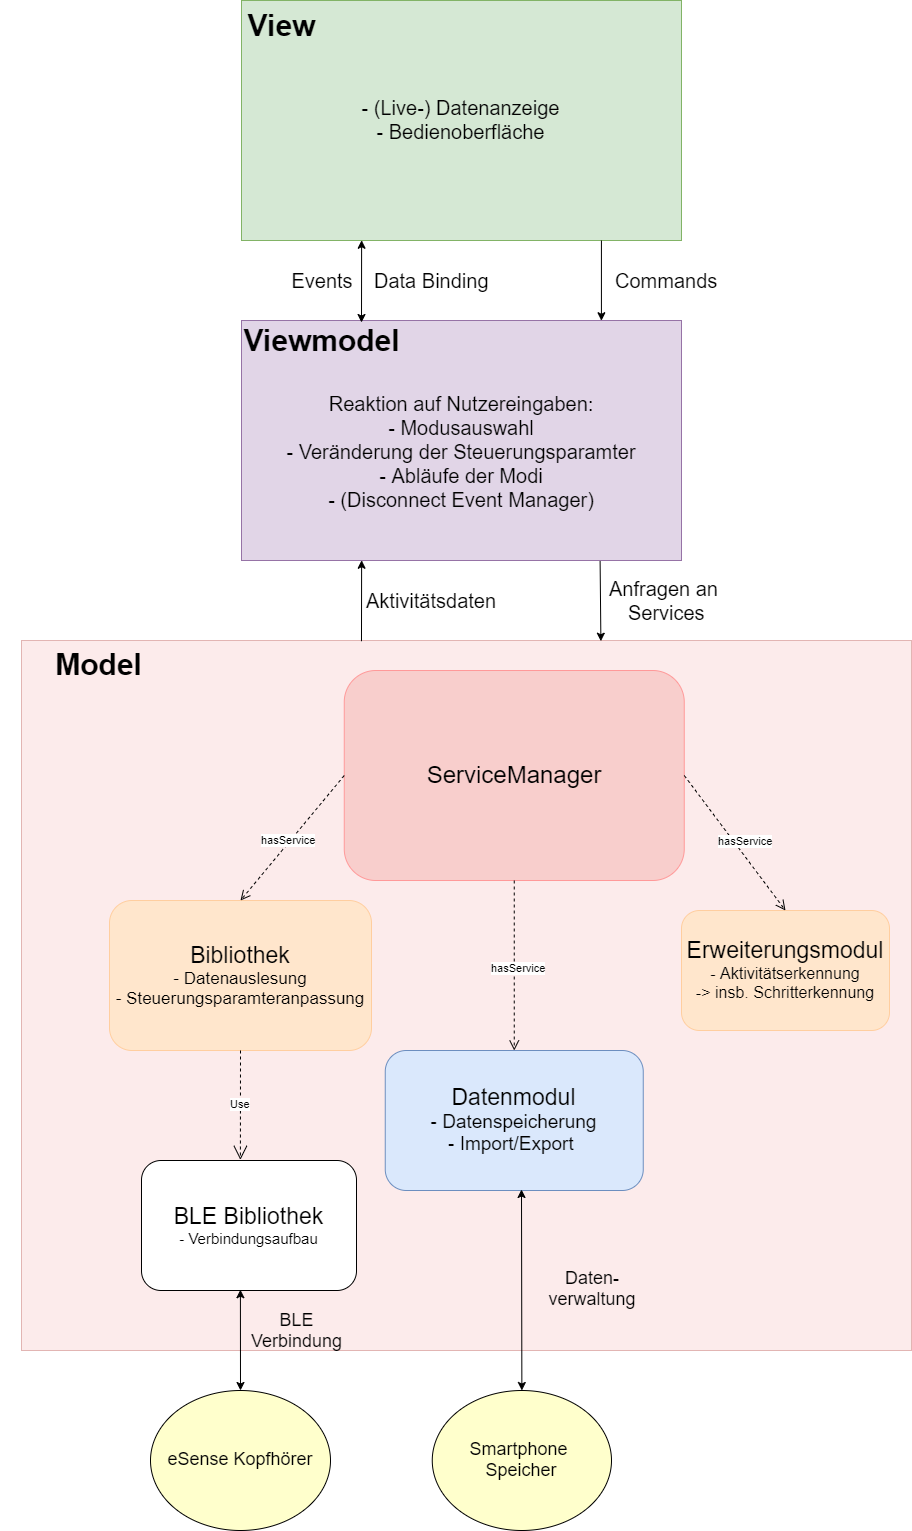
\includegraphics[width=0.8\textwidth]{./Diagramme/ArchitekturdiagrammmitServiceManager.png}
	\end{center}
	\clearpage %%sieht sonst noch zerrissener aus;    Gehts nicht irgendwie schöner? Sodass das Diagramm ganz oben quasi anliegt?
	\subsection{Kurze Erläuterung zum Architekturdiagramm}
Wir haben uns bei der Architekturdiagramm für \textsf{Model-View-ViewModel}, eine Spezialisierung des Entwurfsmusters Model-View-Controller, entschieden. Dabei wurden im Vergleich zum Architekturdiagramm im Pflichtenheft einige kleinere Änderungen vorgenommen. Es folgt eine Beschreibung der Komponenten:
  \begin{itemize}
 	\item \textsf{\glqq Model\grqq{}} enthält die Geschäftslogik der App und ist durch die neu hinzugefügte zentrale Schnittstelle des ServiceManagers stark nach außen abgekapselt. Benötigte Services können beim Programmstart im ServiceManager registriert werden, sodass bei Bedarf eine Singleton-Instanz des Service zur Verfügung gestellt werden kann. Wesentlich sind dabei folgende Services: 
\begin{itemize}
      \item Die Verwaltung der anfallenden Aktivitätsdaten (Abruf und Bereitstellung der gespeicherten Daten in der Datenbank, im CSV-Format) über ein Datenmodul.
      \item Die Bibliothek, die für die Kommunikation mit den \Gls{Earables} (Verbindungsaufbau, Start und Stopp des Samplings, Konfiguration der \Gls{Steuerungsparameter}, Auslesen der Sensordaten) zuständig ist. Dazu wird eine externe Bibliothek\footnote{https://github.com/xabre/xamarin-bluetooth-le} verwendet. Die ausgelesenen Sensordaten werden per Event an die einzelnen Aktivitätsanalysen weiter geschickt. 
      \item Das Erweiterungsmodul, das sich um die Aktivitätserkennung kümmert. Es definiert die unterschiedlichen Analysemethoden für die Aktivitäten, die aufgrund der Servicestruktur leicht austauschbar sind und nutzt die Schnittstellen der Bibliothek. Die erkannten Aktivitätsdaten werden ebenfalls per Event an das ViewModel weiter geschickt. 
\end{itemize}
Die Services sind dabei jeweils unabhängig vom restlichen Model funktionsfähig und dadurch leichter testbar.
\item \textsf{\glqq ViewModel\grqq{}} ist das Bindeglied zwischen View und Model. Es enthält die Logik der Nutzeroberfläche, wird also bei Benutzerinteraktion von der View benachrichtigt. Dabei benutzen wir unter anderem eine Befehlsstruktur, um beispielsweise Buttonklicks zu registrieren und an das ViewModel weiter zu delegieren. Das ViewModel interagiert mit dem Model über die neu hinzugefügte Schnittstelle des ServiceManagers und kann bei ihm Anfragen an benötigte Services wie Aktivitätsanalysen stellen. Darüber hinaus kümmert es sich darum, dass in bestimmten Fällen die View angepasst wird, zum Beispiel bei Verbindungsabbruch zu den \Gls{Earables} und beim Empfangen von neuen Aktivitätsdaten. Dies erfolgt über Databinding und der von Xamarin angebotenen NotifyPropertyChanged Schnittstelle.

\item \textsf{\glqq View\grqq{}} enthält alle grafisch angezeigten Elemente, also die Datenanzeige und Bedienoberfläche der App.
\end{itemize}
  Der Vorteil dieser Architektur ist eine klare Trennung von Benutzerinteraktion und Programmlogik sowie eine lose Kopplung zwischen einzelnen Funktionalitäten insbesondere durch die Eventstruktur, was die Flexibilität und das modulare Testen deutlich erleichtert.
\clearpage
  \subsection{Klassendiagramm}
  \begin{center}
	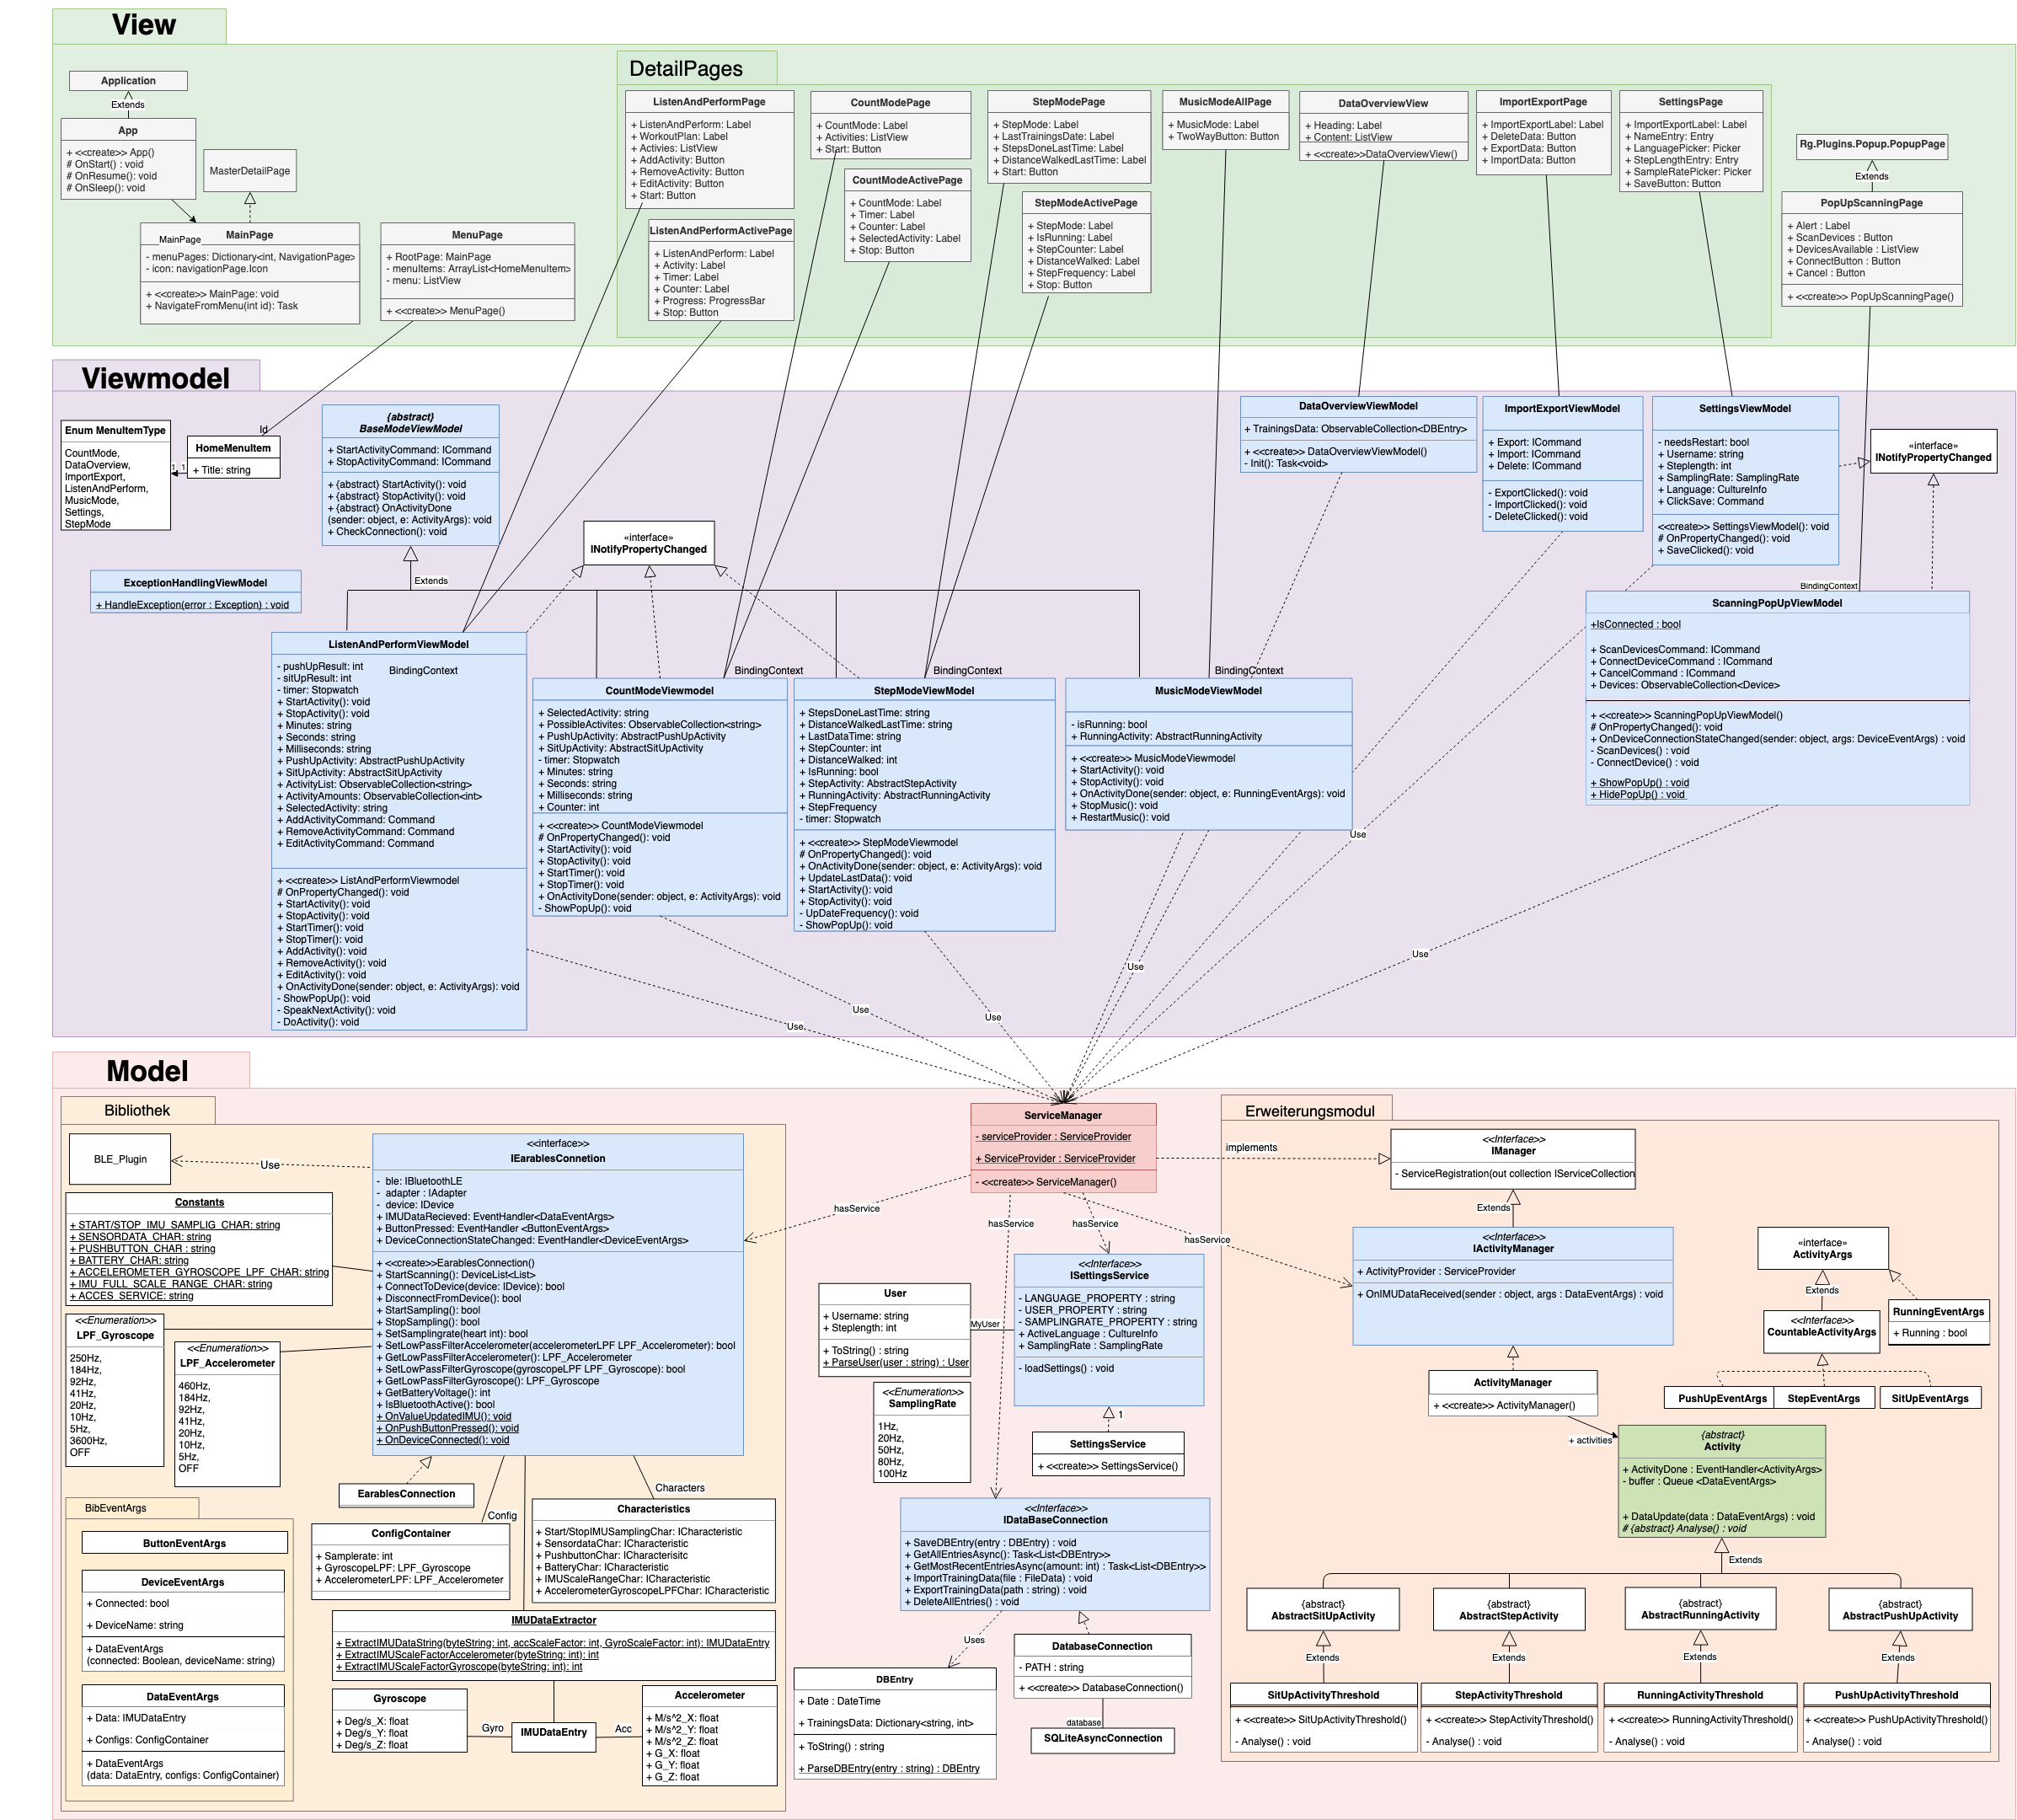
\includegraphics[width=\textwidth]{Diagramme/uebersicht/Klassendiagram_KOMPAKT.png}
\end{center}
\paragraph{Anmerkungen}
Eine hochauflösendere Darstellung des Klassendiagramms findet sich im Anhang.
\clearpage
%%\section{Klassenübersicht} brauchen wir nicht, da das bei uns schon alles im Inhaltsverzeichnis aufgelistet wird.
\section{Klassenbeschreibung Model}
\subsection{Bibliothek}
\begin{center}
	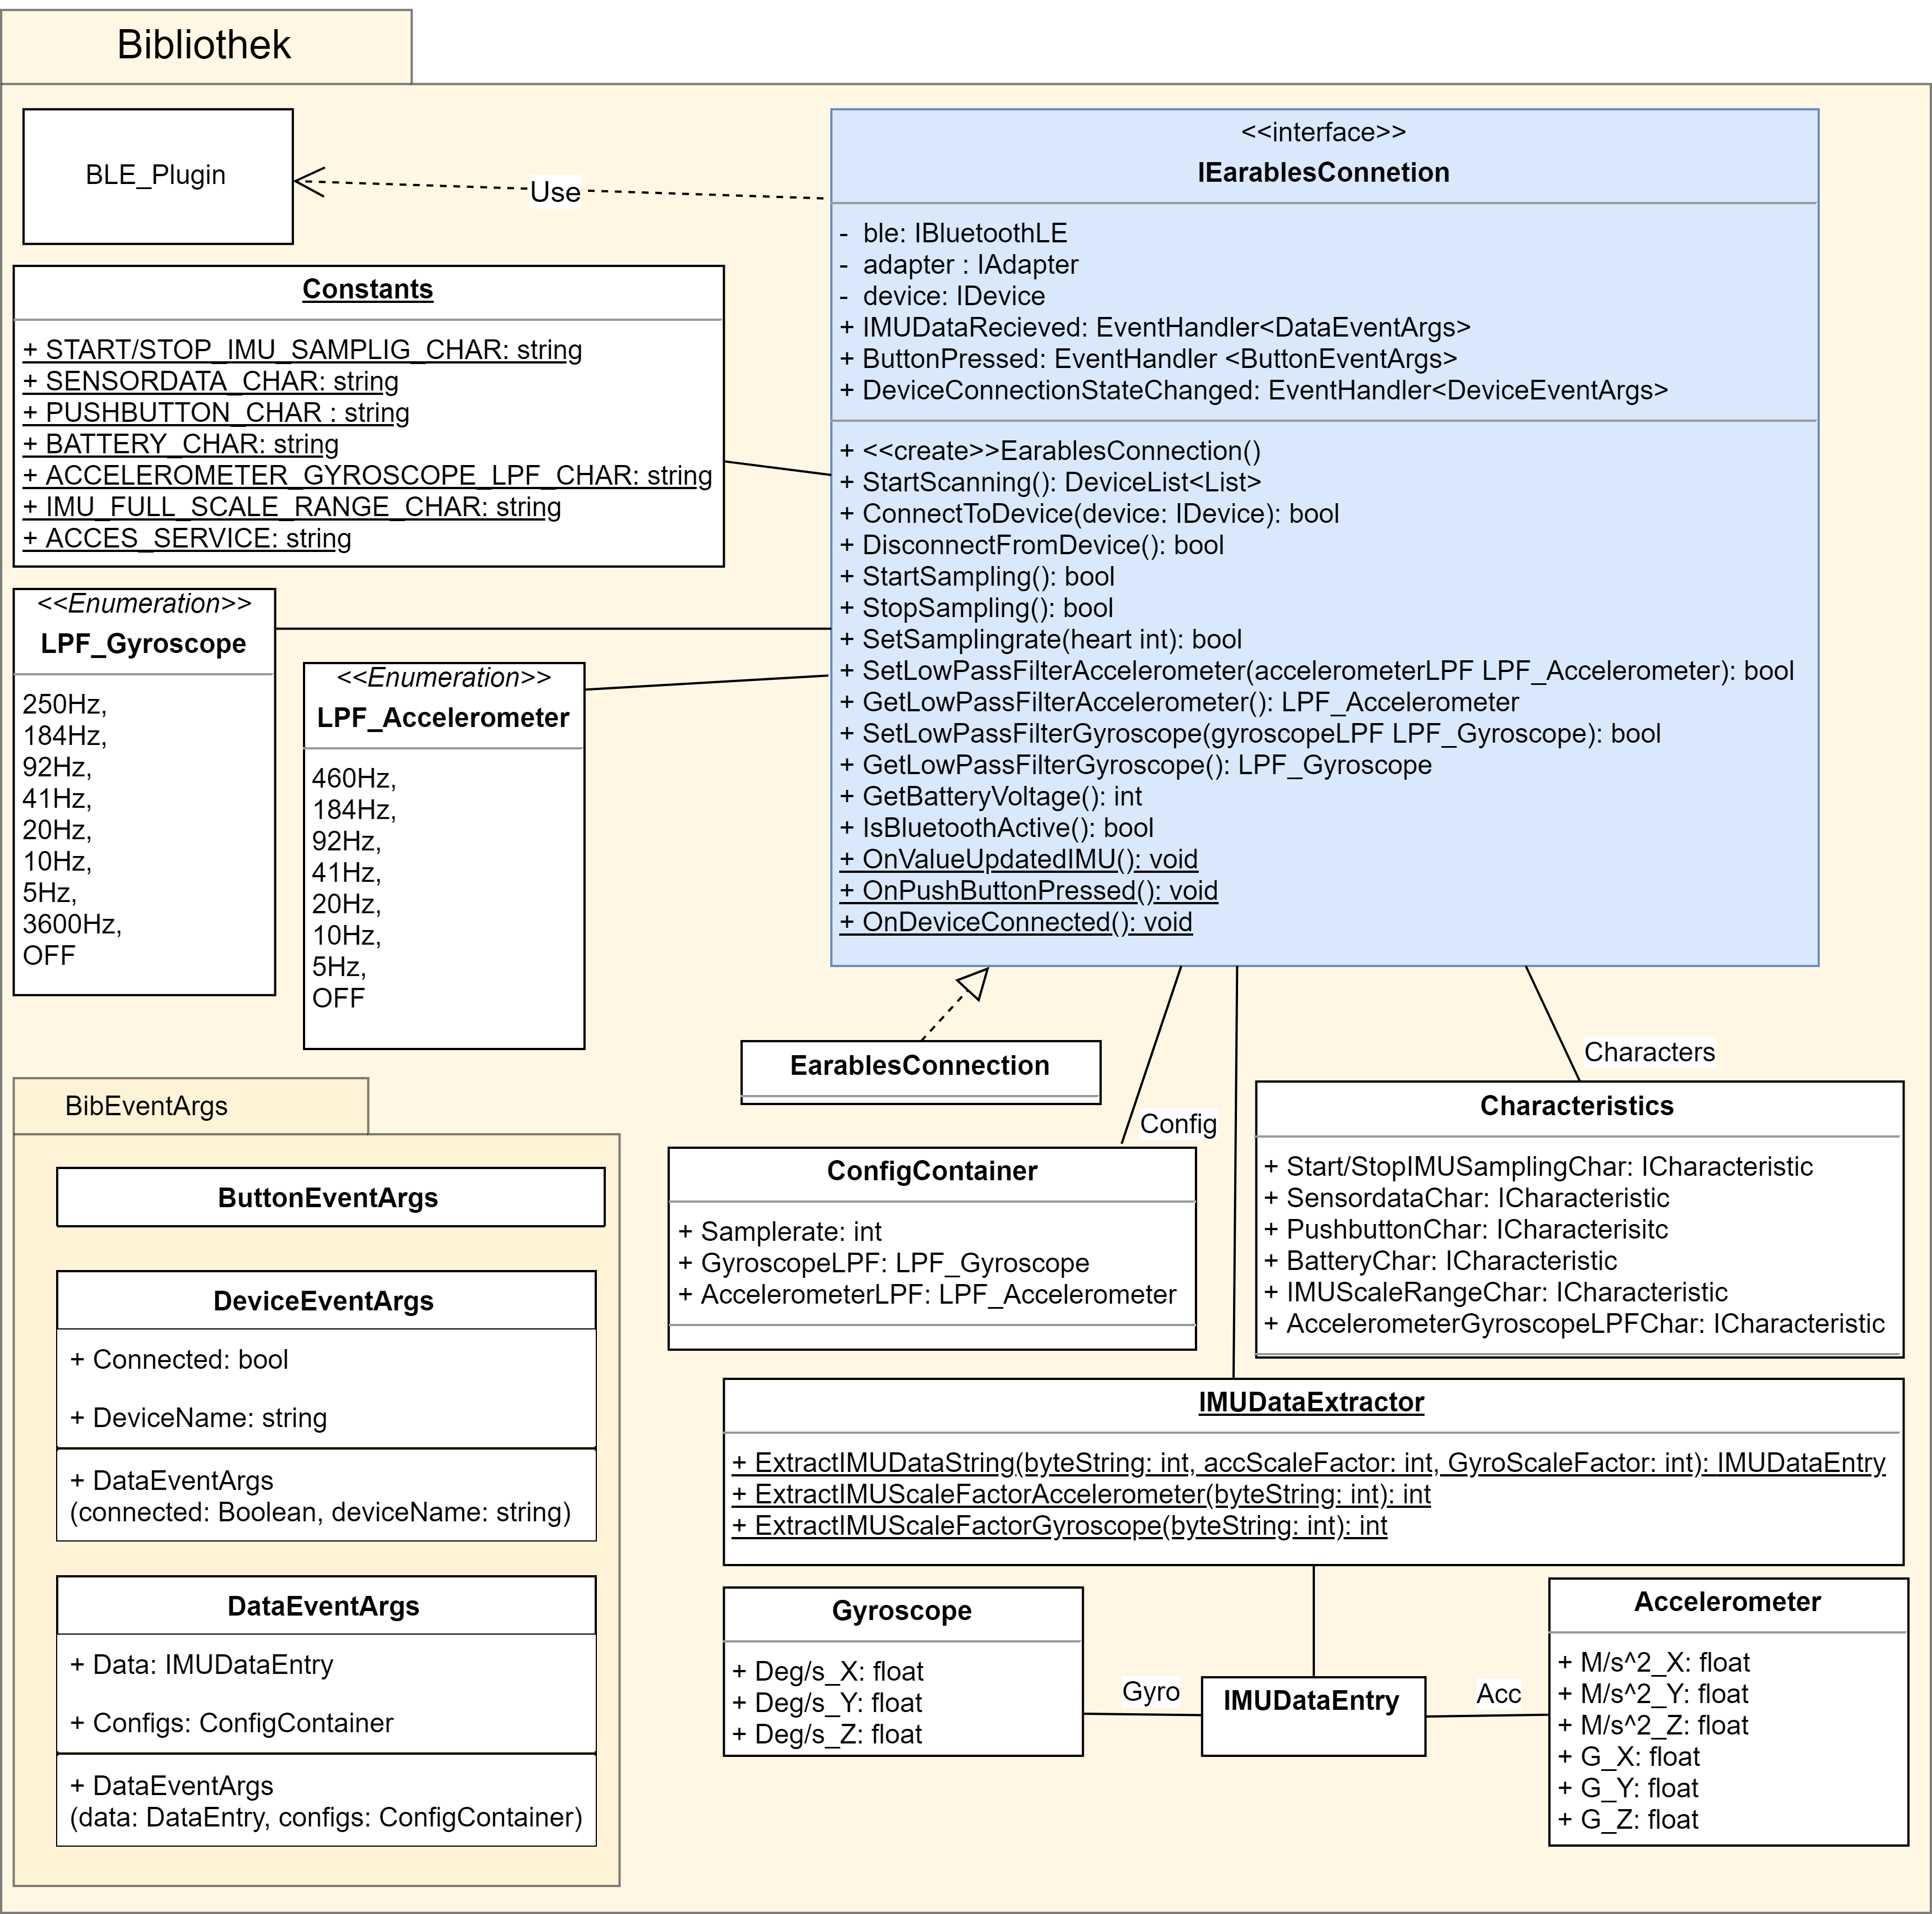
\includegraphics[width=\textwidth]{Diagramme/uebersicht/Bibliothek.png}
\end{center}	
\subsubsection{Interface IEarablesConnection}
	
	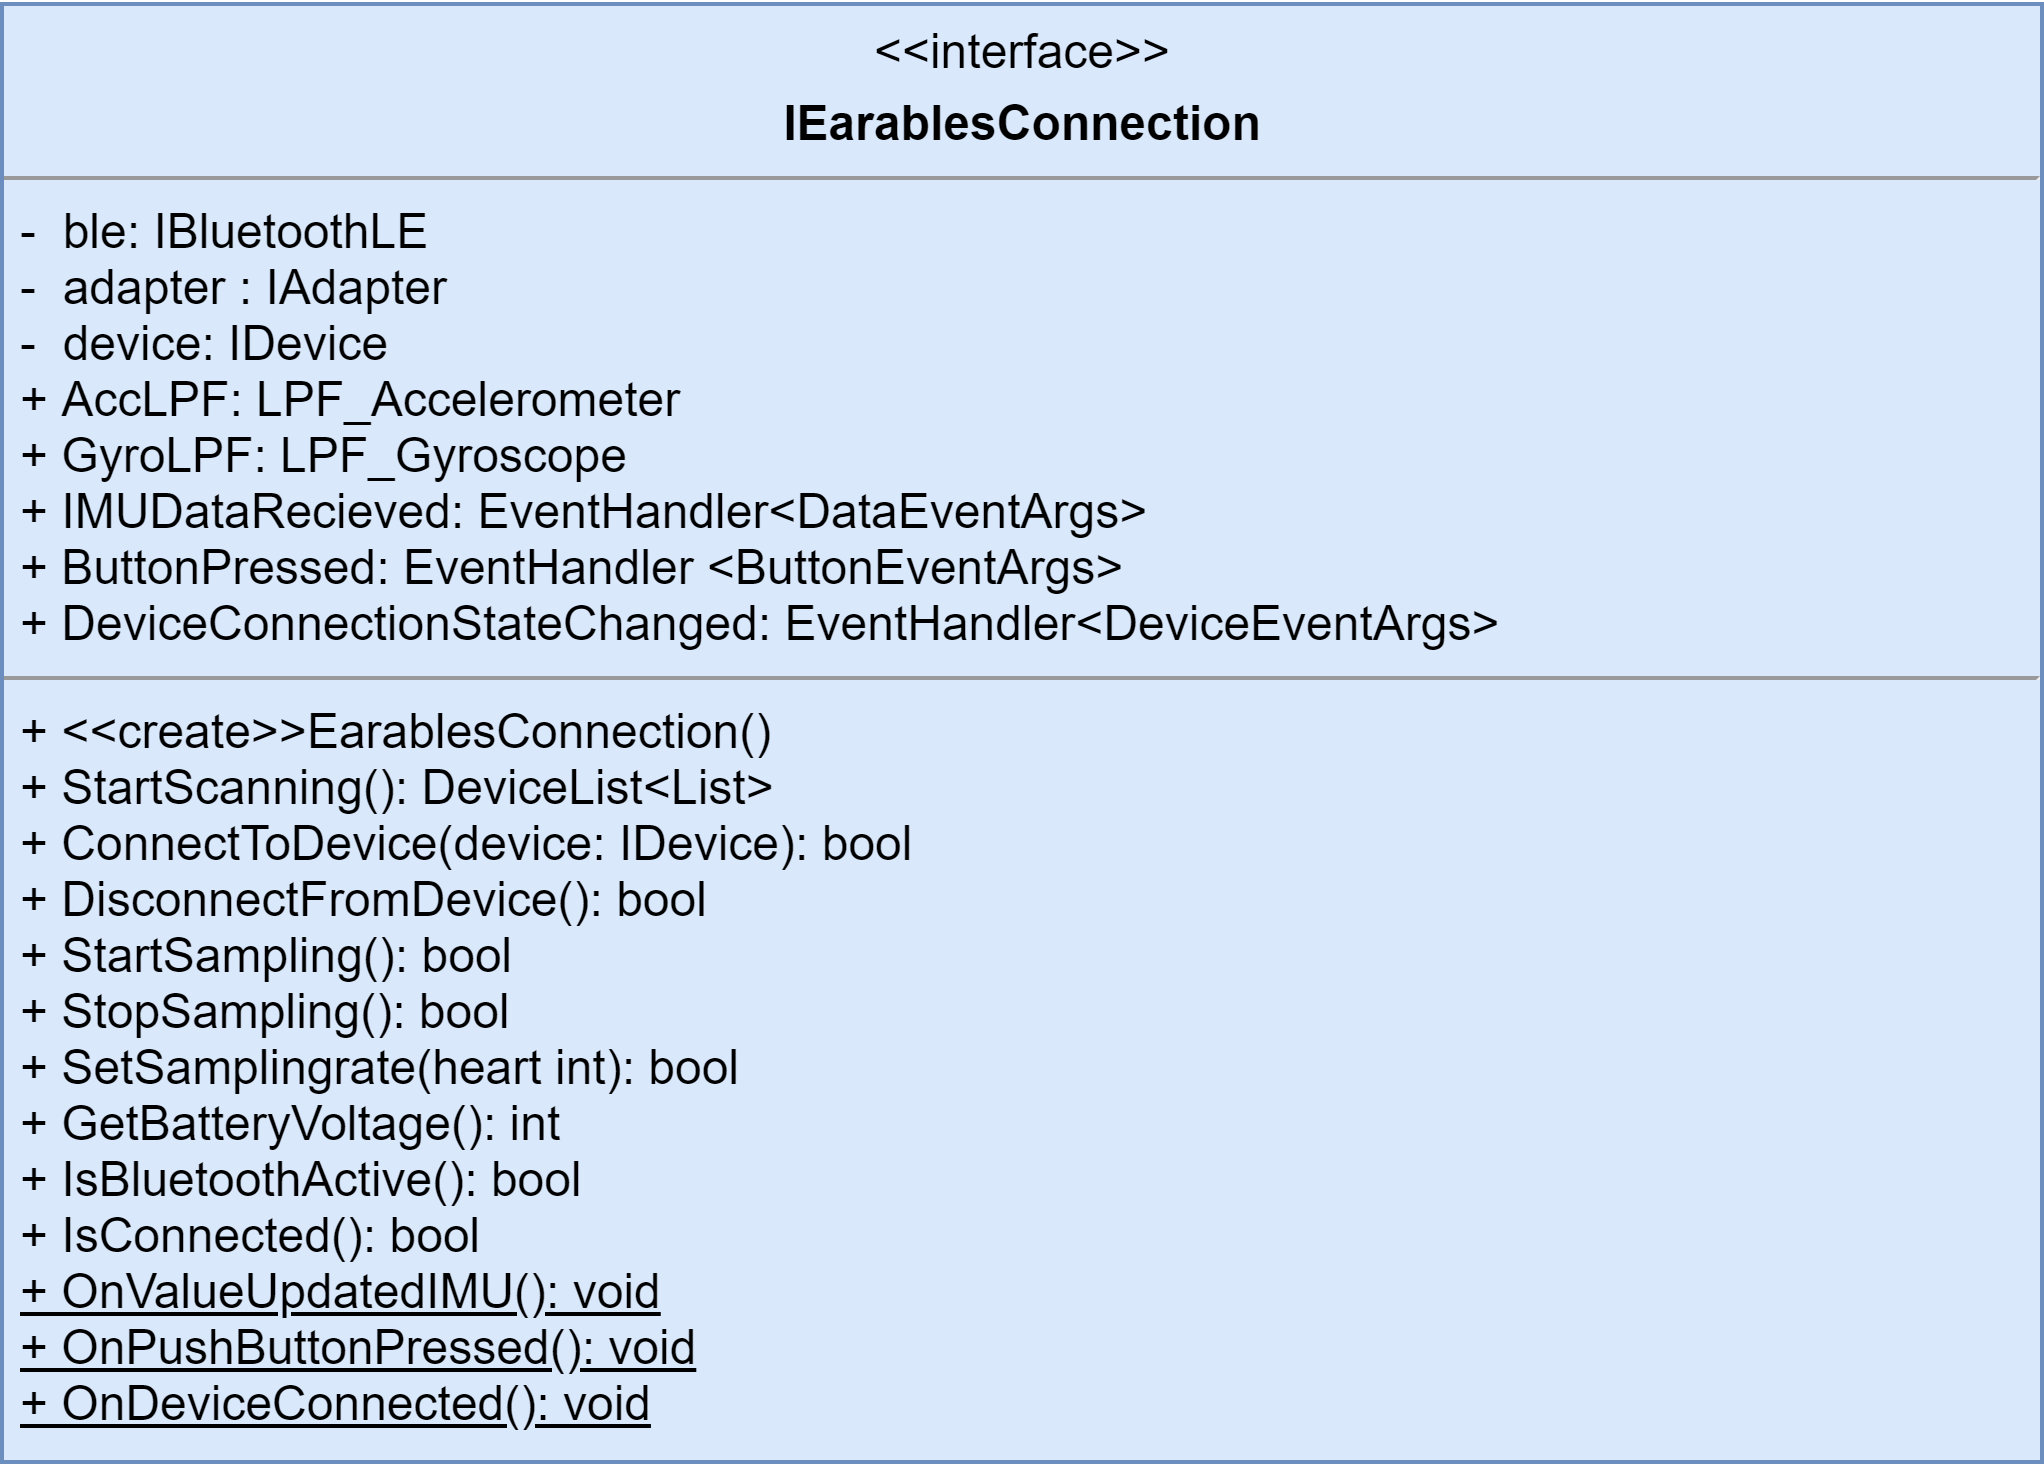
\includegraphics[width=\textwidth]{bilder/BibPackageKlassen/IEarablesConnection.png}

\paragraph{Klassenbeschreibung:}
Diese Klasse ist das Herz der Bibliothek. Sie ist die Schnittstelle, über die später kommuniziert werden kann. Hierbei handelt es sich um ein Interface um Mocking zu ermöglichen und so das Implementieren und Testen zu vereinfachen. Um eine BLE Verbindung herzustellen benutzt sie das \glqq \gls{Bluetooth LE Plugin}\grqq{}\footnote{https://github.com/xabre/xamarin-bluetooth-le}.
\paragraph{Attribute:}
\begin{itemize}
	\item[$-$] \textbf{ble: IBluetoothLE}\\ Wird benötigt um auf die Bluetooth Funktion des Smartphones zuzugreifen. Der Typ IBluetooth befindet sich im BLE\_Plugin.
	\item[$-$] \textbf{adapter: IAdapter}\\ Wird benötigt um die Bluetooth Verbindung aufzubauen. Das Attribut repräsentiert das Smartphone. Der Typ  IAdapter befindet sich im BLE\_Plugin.
	\item[$-$] \textbf{device: IDevice}\\ Wird benötigt um die Bluetooth Verbindung aufzubauen. Das Attribut repräsentiert das Gerät mit dem man sich verbinden möchte. Der Typ  IDevice befindet sich im BLE\_Plugin.
	\item[+] \textbf{AccLPF: LPF\_Accelerometer}\\ Dient als Property. Die Setter und Getter setzen/holen das AccelerometerLPF Attribut der Instanz Config.
	\item[+] \textbf{GyroLPF: LPF\_Gyroscope}\\ Dient als Property. Die Setter und Getter setzen/holen das GyroscoperLPF Attribut der Instanz Config.
	\item[+] \textbf{BatteryVoltage: int}\\ Dient als Property. In diesem Property wird die Batterieladung, der \Gls{Earables}, gespeichert. Sie ist immer aktuell, da sie automatisch aktualisiert wird, wenn sich der Batteriestatus, der \Gls{Earables} ändert.
	\item[+] \textbf{IMUDataReceived: EventHandler<DataEventArgs>}\\ Das Event welches gefeuert wird, wenn neue IMU Daten vorliegen.
	\item[+] \textbf{ButtonPressed: EventHandler <ButtonEventArgs>}\\ Das Event, welches gefeuert wird, wenn der Knopf, der Earables gedrückt wurde.
	\item[+] \textbf{DeviceConnectionStateChanged: EventHandler<DeviceEventArgs>}\\ Das Event welches gefeuert wird, wenn sich der Verbindungsstatus der Earables ändert.
	\item[+] \textbf{Config: ConfigContainer}\\ In diesem Attribut befinden sich die Konfigurationsvariablen für die \Gls{Earables}.
	\item[+] \textbf{Characters: Characteristic}\\ Das Attribut enthält alle Charakteristiken die angesprochen werden müssen.
\end{itemize}
\paragraph{Methoden:}
\begin{itemize}
	\item[+] \textbf{<<create>>\Gls{Earables}Connection()}\\ Im Konstruktor werden die Attribute ble und adapter initialisiert.
	\item[+] \textbf{StartScanning(): DeviceList<List>}\\ Diese Methode legt eine neue Liste vom Typ IDevice an, in der sie alle gefundenen Devices speichert und anschließend zurückgibt. Sie benutzt die Methoden DeviceDiscovered und StartScanningForDevicesAsync aus dem Interface IAdapter.
	\item[+] \textbf{ConnectToDevice(device: Idevice): bool}\\ Mit dieser Methode kann sich der Nutzer mit einem Bluetooth fähigen Gerät verbinden. Er gibt das Device, mit dem er sich verbinden möchte, als Parameter mit. Falls die Verbindung erfolgreich war, wird true zurückgegeben. Konnte keine Verbindung hergestellt werden, wird false zurückgegeben. Hierbei wird die Methode ConnectToDeviceAsync aus dem BLE\_Pugin der Klasse IAdapter zur Hilfe genommen. Zusätzlich werden gleich alle benötigten Charakteristiken geladen und abgespeichert, um sie nicht immer neu laden zu müssen, wenn sie gebraucht werden. Das geschieht mithilfe der Methoden GetServiceAsync und GetCharacteristicAsync aus dem BLE\_Plugin. Zum Schluss werden noch die Handler für die entsprechenden Events registriert und die Aktualisierung mit der Methode StartUpdatesAsync, aus dem BLE\_Plugin, gestartet.
	\item[+] \textbf{DisconnectFromDevice(): bool}\\ Falls das Gerät eine Verbindung zu einem Device besitzt, wird diese getrennt und es wird true zurückgegeben. Wenn das Gerät keine Verbindung besitzt, passiert nichts und es wird false zurückgegeben. Tritt ein Fehler beim Trennen auf, wird ebenfalls false zurückgegeben. Zum Trennen der Verbindung wird die Methode DisconnectDeviceAsync aus dem BLE\_Pugin der Klasse IAdapter benutzt.
	\item[+] \textbf{StartSampling(): bool}\\ Diese Methode startet die Datenaufzeichnung des IMU. Falls die Datenaufzeichnung erfolgreich gestartet wurde, wird true zurückgegeben, ansonsten false. Die Methode WriteAsync aus dem BLE\_Plugin ermöglicht es die Charakteristik zu beschreiben. Hinweis: Ist die Samplingrate nicht gesetzt, so wird die Standarteinstellung genommen.
	\item[+] \textbf{StopSampling(): bool}\\Die Datenaufzeichnung des IMU wird mit dieser Methode gestoppt. Falls die Datenaufzeichnung erfolgreich gestoppt wurde, wird true zurückgegeben, ansonsten false. Die Methode WriteAsync aus dem BLE\_Plugin ermöglicht es die Charakteristik zu beschreiben.
	\item[+] \textbf{SetSamplingrate(heart int): bool}\\Die Samplingrate wird gesetzt und gespeichert. Bei erfolgreichem Setzen wird true zurückgegeben, ansonsten false. Die Methode WriteAsync aus dem BLE\_Plugin ermöglicht es die Charakteristik zu beschreiben.
	\item[+] \textbf{IsBluetoothActive(): bool}\\ Zeigt an ob Bluetooth auf dem Smartphone aktiviert ist. Gibt true zurück falls Bluetooth aktiviert ist und false, falls nicht.
	\item[+] \textbf{IsConnected(): bool}\\ Gibt true zurück falls eine Bluetoothverbindung, zu einem Gerät existiert. Ansonsten wird false zurück gegeben.
	\item[+] \textbf{static OnValueUpdatedIMU(): void}\\ Falls neue IMU Daten vorliegen, wird diese Methode aufgerufen und feuert das Event IMUDataReceived.
	\item[+] \textbf{static OnPushButtonPressed(): void}\\ Falls der Knopf an den \Gls{Earables} gedrückt wurde, wird diese Methode aufgerufen und feuert das Event ButtonPressed.
	\item[+] \textbf{static OnDeviceConnected(): void}\\ Falls eine Verbindung mit einem Device hergestellt wurde oder eine bestehende Verbindung aufgelöst wurde, wird diese Methode aufgerufen und feuert das Event DeviceConnectionStateChanged.
\end{itemize}

\begin{minipage}[t]{0.7\textwidth}
	\subsubsection{Class EarablesConnection}
\end{minipage}
\begin{minipage}[c]{0.3\textwidth}
	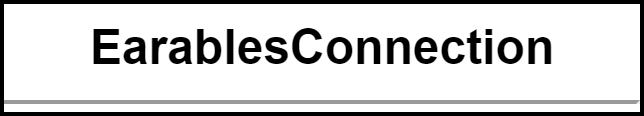
\includegraphics[width=\textwidth]{bilder/BibPackageKlassen/EarablesConnection}
\end{minipage}

\paragraph{Klassenbeschreibung:}
Die Klasse EarablesConnection implementiert das IEarablesConnection Interface und ist die konkrete Klasse, die sich um die BLE-Verbindung kümmert.\\

\begin{minipage}[b]{0.5\textwidth}
	\subsubsection{Static Class Constants}
	
	\end{minipage}
	\begin{minipage}[c]{0.5\textwidth}
	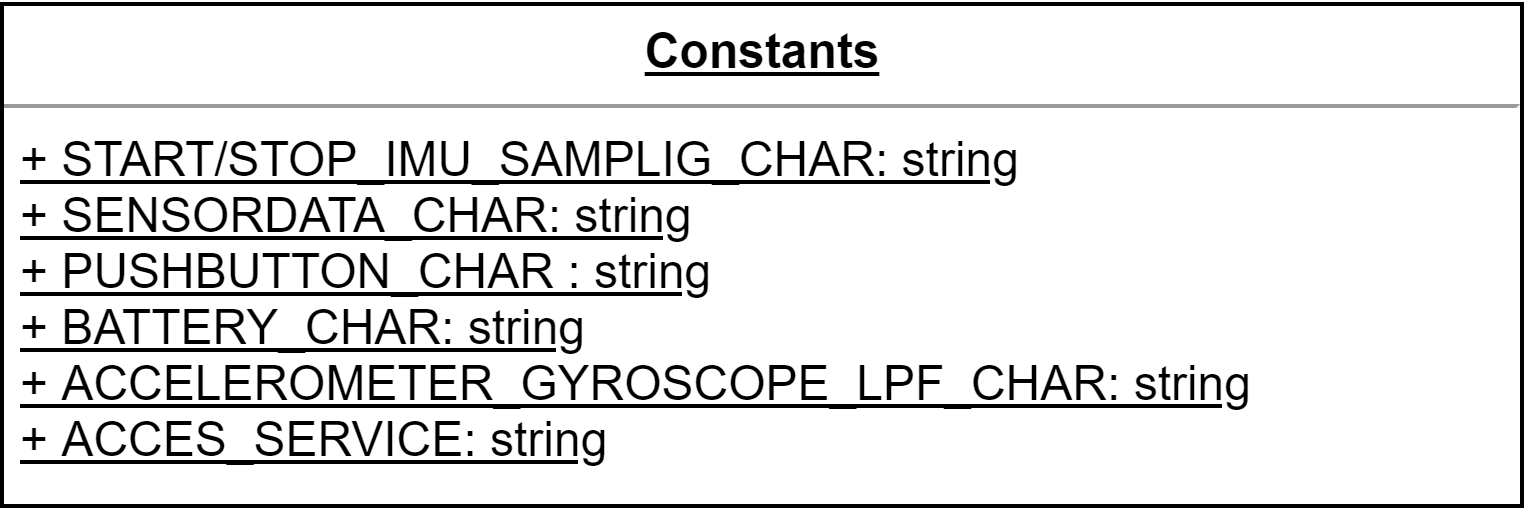
\includegraphics[width=\textwidth]{bilder/BibPackageKlassen/Constants.png}
\end{minipage}

\paragraph{Klassenbeschreibung:}
Die Constants Klasse enthält alle Konstanten, die benötigt werden, um die entsprechenden Service und Charakteristiken aus den \Gls{Earables} zu lesen. Sie ist als static gekennzeichnet, da sie nur Konstanten bereitstellt und sonst keine weitere Funktionalität beinhaltet.

\paragraph{Attribute:}
\begin{itemize}
	\item[+] \textbf{START/STOP\_IMU\_SAMPLIG\_CHAR: string}\\ Dieser string enthält die Beschreibung der Charakteristik, welche beschrieben wird,  um das IMU Daten Sampling zu starten und zu stoppen.
	\item[+] \textbf{SENSORDATA\_CHAR: string}\\ Dieser string enthält die Beschreibung der Charakteristik, in dem die IMU Sensordaten gespeichert werden.
	\item[+] \textbf{PUSHBUTTON\_CHAR: string} \\Dieser string enthält die Beschreibung der Charakteristik, in dem der Push Button Status gespeichert wird.
	\item[+] \textbf{BATTERY\_CHAR: string}\\ Dieser string enthält die Beschreibung der Charakteristik, in dem die Batterieladung gespeichert wird.
	\item[+] \textbf{ACCELEROMETER\_GYROSCOPE\_LPF\_CHAR: string}\\ Dieser string enthält die Beschreibung der Charakteristik, welche beschrieben wird, um den Low Pass Filter für den Accelerometer und das Gyroscope zu setzen.
\item[+] \textbf{ACCESS\_SERVICE: string}\\ Dieser string enthält die Beschreibung des Service Access-Service, der alle benötigten Charakteristiken enthält.\\
\end{itemize}

\begin{minipage}[t]{0.7\textwidth}
	\subsubsection{Enumeration LPF\_Gyroscope}
	\end{minipage}
	\begin{minipage}[c]{0.3\textwidth}
	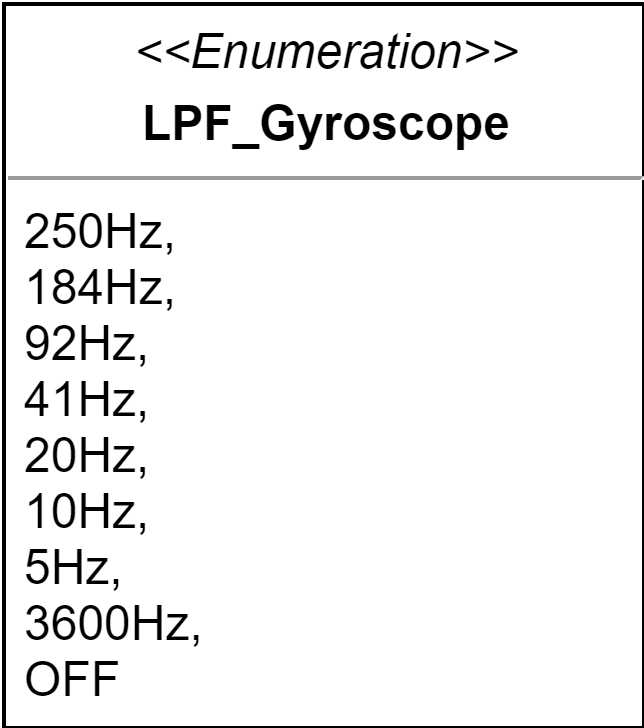
\includegraphics[width=\textwidth]{bilder/BibPackageKlassen/LPF_Gyrosope.png}
\end{minipage}

\paragraph{Klassenbeschreibung:}
Dieses Enum beinhaltet alle möglichen LPF Werte, die der LPF für das Gyroscope annehmen kann.

\paragraph{Werte:}
\begin{itemize}
	\item \textbf{250Hz}\\Steht dafür, dass der LPF 250 Hz annehmen kann.
	\item \textbf{184Hz}\\Steht dafür, dass der LPF 184 Hz annehmen kann.
	\item \textbf{92Hz}\\Steht dafür, dass der LPF 92 Hz annehmen kann.
	\item \textbf{41Hz}\\Steht dafür, dass der LPF 41 Hz annehmen kann.
	\item \textbf{20Hz}\\Steht dafür, dass der LPF 20 Hz annehmen kann.
	\item \textbf{10Hz}\\Steht dafür, dass der LPF 10 Hz annehmen kann.
	\item \textbf{5Hz}\\Steht dafür, dass der LPF 5 Hz annehmen kann.
	\item \textbf{3600Hz}\\Steht dafür, dass der LPF 3600 Hz annehmen kann.
	\item \textbf{OFF}\\Steht dafür, dass der LPF aus ist.\\
\end{itemize}


\begin{minipage}[b]{0.7\textwidth}
	\subsubsection{Enumeration LPF\_Accelerometer}
	
	\end{minipage}
	\begin{minipage}[c]{0.3\textwidth}
	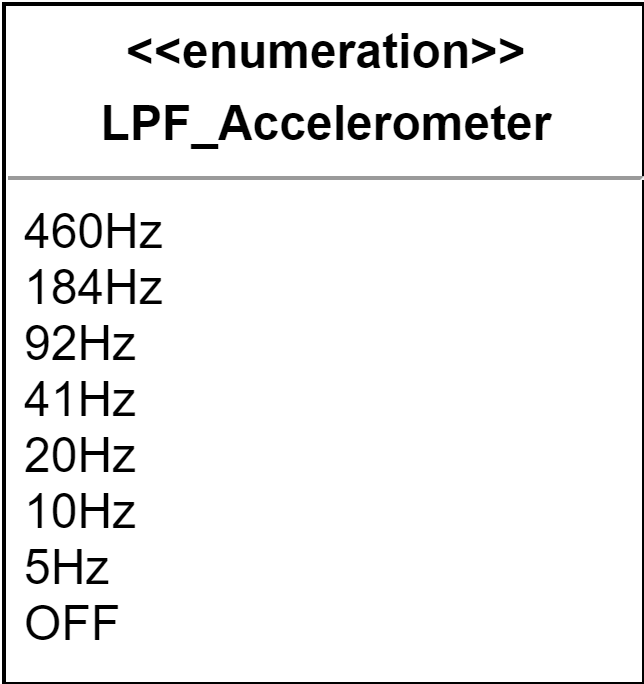
\includegraphics[width=\textwidth]{bilder/BibPackageKlassen/LPF_Accelerometer.png}
\end{minipage}
\paragraph{Klassenbeschreibung:}
Dieses Enum beinhaltet alle möglichen LPF Werte, die der LPF für das Accelerometer annehmen kann.

\paragraph{Werte:}
\begin{itemize}
	\item \textbf{460Hz}\\Steht dafür, dass der LPF 460 Hz annehmen kann.
	\item \textbf{184Hz}\\Steht dafür, dass der LPF 184 Hz annehmen kann.
	\item \textbf{92Hz}\\Steht dafür, dass der LPF 92 Hz annehmen kann.
	\item \textbf{41Hz}\\Steht dafür, dass der LPF 41 Hz annehmen kann.
	\item \textbf{20Hz}\\Steht dafür, dass der LPF 20 Hz annehmen kann.
	\item \textbf{10Hz}\\Steht dafür, dass der LPF 10 Hz annehmen kann.
	\item \textbf{5Hz}\\Steht dafür, dass der LPF 5 Hz annehmen kann.
	\item \textbf{OFF}\\Steht dafür, dass der LPF aus ist.\\
\end{itemize}

\begin{minipage}[b]{0.7\textwidth}
	\subsubsection{Class ConfigContainer}
	\end{minipage}
	\begin{minipage}[c]{0.3\textwidth}
	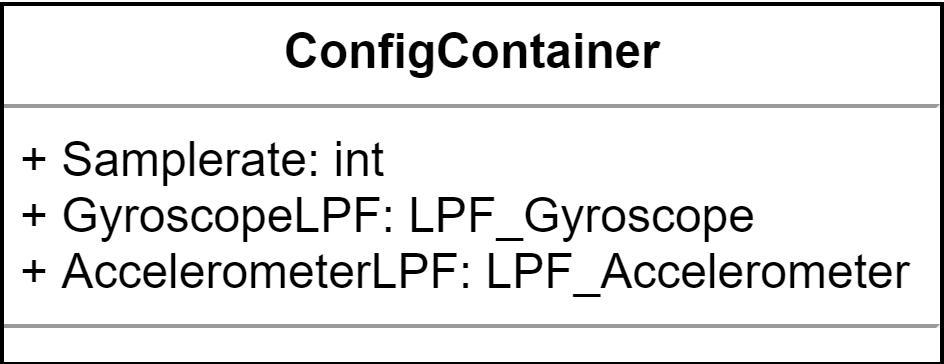
\includegraphics[width=\textwidth]{bilder/BibPackageKlassen/ConfigContainer.png}
\end{minipage}
\paragraph{Klassenbeschreibung:}
Diese Klasse beinhaltet alle Einstellungsmöglichkeiten für die \Gls{Earables}.

\paragraph{Attribute:}
\begin{itemize}
	\item[+] \textbf{Samplerate: int}\\Hier wird die Samplerate gespeichert, in der die \Gls{Earables} neue Daten des IMU aufzeichnen.
	\item[+] \textbf{GyroscopeLPF: LPF\_Gyroscope}\\Dieses Attribut enthält den aktuell eingestellten LPF für das Gyroscope.
	\item[+] \textbf{AccelerometerLPF: LPF\_Accelerometer}\\Dieses Attribut enthält den aktuell eingestellten LPF für den Accelerometer.
\end{itemize}


	\subsubsection{Static Class IMUDataExtractor}

	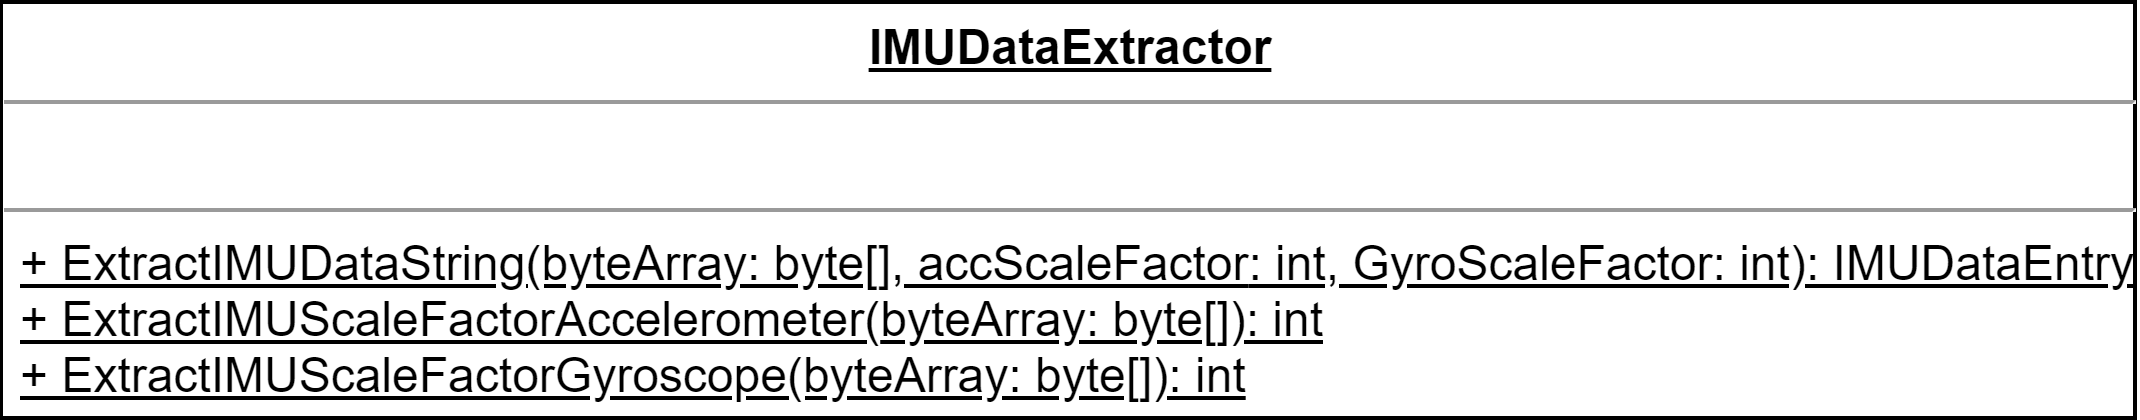
\includegraphics[width=\textwidth]{bilder/BibPackageKlassen/IMUDataExtractor.png}

\paragraph{Klassenbeschreibung:}
Diese Klasse übernimmt das Umwandeln des Bit strings in vernünftige Werte und Einheiten.
Die Klasse wurde erstellt um dem IEarablesConnection Interface Arbeit abzunehmen und Logik zu entkoppeln, sodass sich das IEarablesConnection
Interface nur um die Kommunikation mit den \Gls{Earables} kümmern muss. Sie ist static, da sie nur einen Dienst anbietet.

\paragraph{Methoden:}
\begin{itemize}
	\item[+] \textbf{ExtractIMUDataString(byteArray: byte[], accScaleFactor: int, GyroScaleFactor): IMUDataEntry}\\Diese Methode erstellt aus dem übergebenen Bytearray ein IMUDataEntry, indem sie die Informationen aus dem Bytearray auswertet und in verschiedene Einheiten umrechnet. Zum Umrechnen benötigt sie noch den accScaleFactor und den gyroScaleFactor. Sie erzeugt ein neues IMUDataEntry Objekt und gibt es als Rückgabewert zurück.
	\item[+] \textbf{ExtractIMUScaleFactorAccelerometer(byteArray: byte[]): int}\\Diese Methode berechnet aus dem übergebenen Bytearray den Scale Factor für den Accelerometer, der beim extrahieren der IMU Daten gebraucht wird, und gibt diesen als Rückgabewert zurück.
	\item[+] \textbf{ExtractIMUScaleFactorGyroscope(byteArray: byte[]): int}\\Diese Methode berechnet aus dem übergebenen Bytearray den Scale Factor für das Gyroscope, der beim extrahieren der IMU Daten gebraucht wird, und gibt diesen als Rückgabewert zurück.
\end{itemize}


\begin{minipage}[b]{0.7\textwidth}
	\subsubsection{Class IMUDataEntry}
	
	\end{minipage}
	\begin{minipage}[c]{0.3\textwidth}
	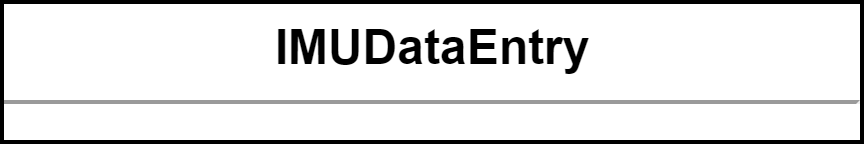
\includegraphics[width=\textwidth]{bilder/BibPackageKlassen/IMUDataEntry.png}
\end{minipage}
\paragraph{Klassenbeschreibung:}
Diese Klasse besitzt alle ausgewerteten IMU Informationen, die in einem Datensatz von den \Gls{Earables} ankommen.

\paragraph{Attribute:}
\begin{itemize}
	\item[+] \textbf{Gyro: Gyroscope}\\In diesem Attribut sind die gemessenen Werte des Gyroscopes enthalten.
	\item[+] \textbf{Acc: Accelerometer}\\In diesem Attribut sind die gemessenen Werte des Accelerometers enthalten.
\end{itemize}

\begin{minipage}[b]{0.7\textwidth}
	\subsubsection{Class Gyroscope}
	
	\end{minipage}
	\begin{minipage}[c]{0.3\textwidth}
	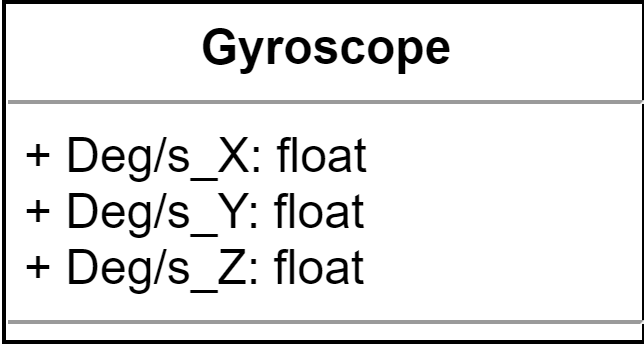
\includegraphics[width=\textwidth]{bilder/BibPackageKlassen/Gyroscope.png}
\end{minipage}
\paragraph{Klassenbeschreibung:}
Diese Klasse besitzt alle ausgewerteten Gyroskopdaten.

\paragraph{Attribute:}
\begin{itemize}
	\item[+] \textbf{Deg/s\_X: float}\\Gibt an um wie viel Grad pro Sekunde sich die \Gls{Earables} in X Richtung gedreht haben.
	\item[+] \textbf{Deg/s\_Y: float}\\Gibt an um wie viel Grad pro Sekunde sich die \Gls{Earables} in Y Richtung gedreht haben.
	\item[+] \textbf{Deg/s\_Z: float}\\Gibt an um wie viel Grad pro Sekunde sich die \Gls{Earables} in Z Richtung gedreht haben.
\end{itemize}

\begin{minipage}[b]{0.7\textwidth}
	\subsubsection{Class Accelerometer}
	\end{minipage}
	\begin{minipage}[c]{0.3\textwidth}
	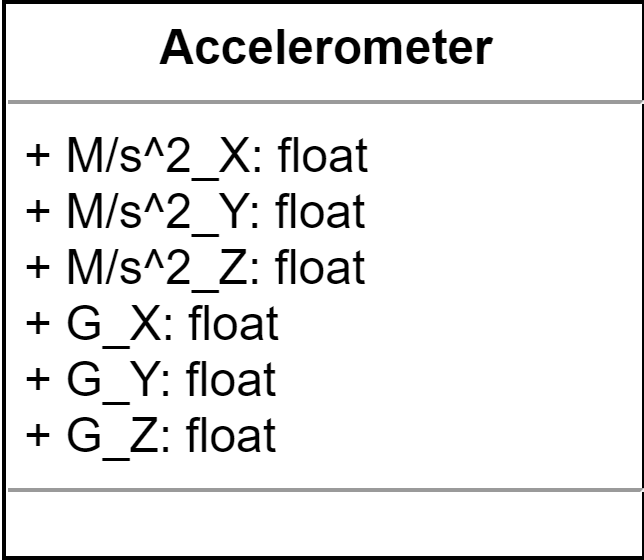
\includegraphics[width=\textwidth]{bilder/BibPackageKlassen/Accelerometer.png}
\end{minipage}
\paragraph{Klassenbeschreibung:}
Diese Klasse besitzt alle ausgewerteten Accelerometer Daten.

\paragraph{Attribute:}
\begin{itemize}
	\item[+] \textbf{M/s$^2$\_X: float}\\Gibt an um wie viel $m/s^2$ sich die \Gls{Earables} in X Richtung beschleunigt haben.
	\item[+] \textbf{M/s$^2$\_Y: float}\\Gibt an um wie viel $m/s^2$ sich die \Gls{Earables} in Y Richtung beschleunigt haben.
	\item[+] \textbf{M/s$^2$\_Z: float}\\Gibt an um wie viel $m/s^2$ sich die \Gls{Earables} in Z Richtung beschleunigt haben.
	\item[+] \textbf{G\_X: float}\\Gibt an um wie viel G sich die \Gls{Earables} in X Richtung beschleunigt haben.
	\item[+] \textbf{G\_Y: float}\\Gibt an um wie viel G sich die \Gls{Earables} in Y Richtung beschleunigt haben.
	\item[+] \textbf{G\_Z: float}\\Gibt an um wie viel G sich die \Gls{Earables} in Z Richtung beschleunigt haben.
\end{itemize}


\begin{minipage}[b]{0.7\textwidth}
	\subsubsection{Class Characteristics}
	\end{minipage}
	\begin{minipage}[c]{0.3\textwidth}
	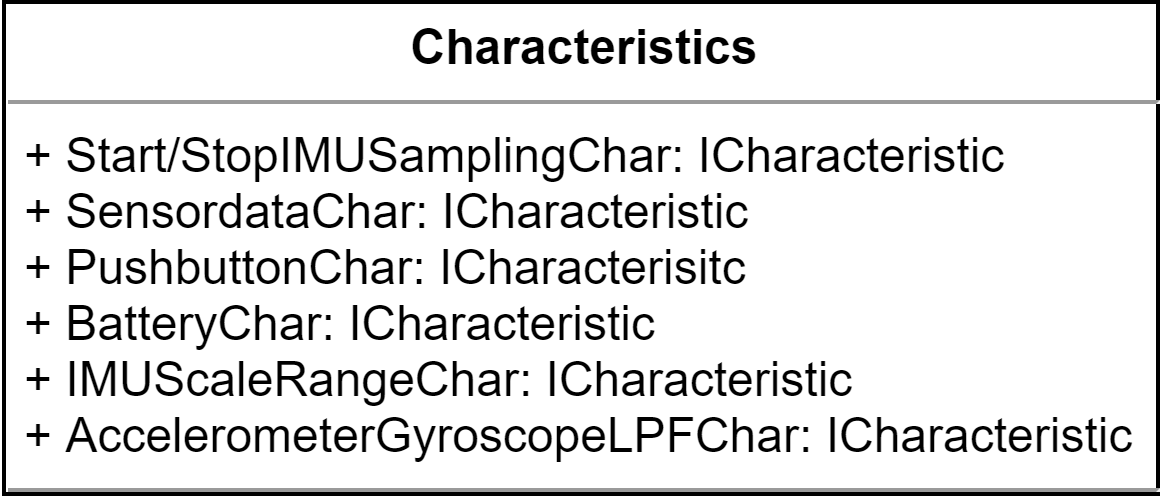
\includegraphics[width=\textwidth]{bilder/BibPackageKlassen/Characteristics.png}
\end{minipage}


\paragraph{Klassenbeschreibung:}
In dieser Klasse werden die Charakteristiken gespeichert, um sie nicht jedes Mal neu laden zu müssen, wenn sie gebraucht werden. Der Datentyp ICharacteristic befindet sich in dem BLE\_Plugin.

\paragraph{Attribute:}
\begin{itemize}
	\item[+] \textbf{Start/StopIMUSamplingChar: ICharacteristic}\\Speichert die Charakteristik, um das IMU Sampling zu starten oder zu stoppen.
	\item[+] \textbf{Sensordata: ICharacteristicChar}\\Speichert die Charakteristik, in der die Sensordaten liegen.
	\item[+] \textbf{Pushbutton: ICharacteristicChar}\\Speichert die Charakteristik, in der der Status des Push Button gespeichert wird.
	\item[+] \textbf{Battery: ICharacteristicChar}\\Speichert die Charakteristik, in der die verbleibende Batterieladung gespeichert wird.
	\item[+] \textbf{AccelerometerGyroscopeLPFChar: ICharacteristic}\\Speichert die Charakteristik, in der die Konfiguration des LPF für den Accelerometer und das Gyroscope geschrieben wird.
\end{itemize}

\begin{minipage}[b]{0.5\textwidth}
	\subsubsection{Class DeviceEventArgs}
	
	\end{minipage}
	\begin{minipage}[c]{0.5\textwidth}
	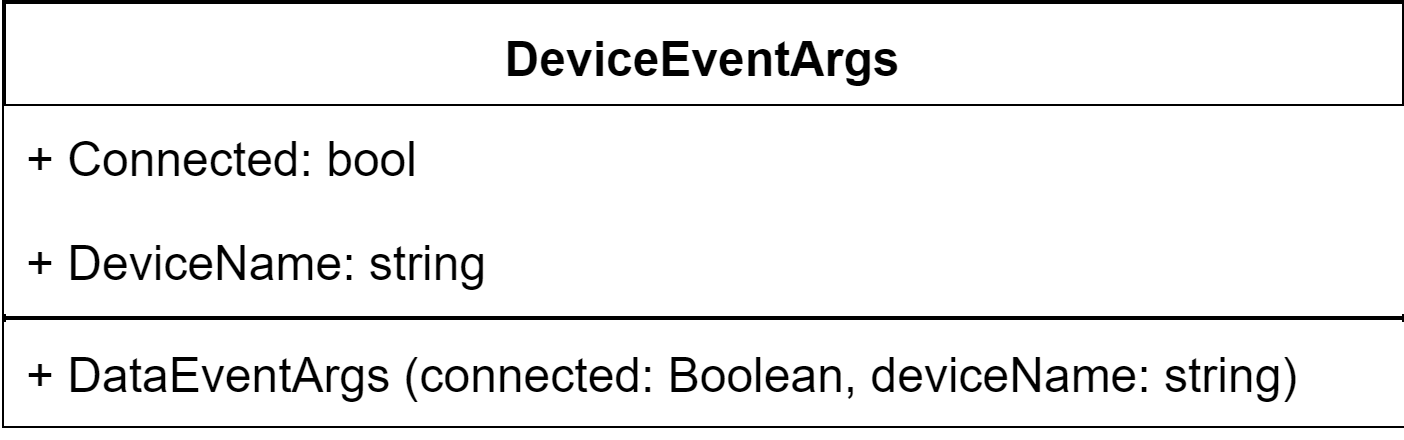
\includegraphics[width=\textwidth]{bilder/BibPackageKlassen/DeviceEventArgs.png}
\end{minipage}
\paragraph{Klassenbeschreibung:}
Enthält alle relevanten Informationen, die als Parameter mit dem Event DeviceConnectionStateChanged gefeuert werden.

\paragraph{Attribute:}
\begin{itemize}
	\item[+] \textbf{Connected: bool}\\Ist true falls eine BLE Verbindung mit einem Device existiert und false falls nicht.
	\item[+] \textbf{DeviceName: string}\\Beinhaltet den Gerätenamen, mit dem das Smartphone verbunden ist. 
\end{itemize}

\paragraph{Methoden:}
\begin{itemize}
	\item[+] \textbf{<<create>>DeviceEventArgs(connected: bool, deviceName: string): void}\\ Zusätzlicher Konstruktor um die Attribute setzten zu können.
\end{itemize}

\begin{minipage}[b]{0.5\textwidth}
	\subsubsection{Class ButtonEventArgs}
	
	\end{minipage}
	\begin{minipage}[c]{0.5\textwidth}
	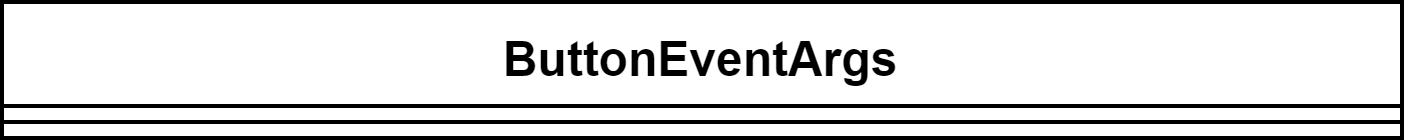
\includegraphics[width=\textwidth]{bilder/BibPackageKlassen/ButtonEventArgs.png}
\end{minipage}
\paragraph{Klassenbeschreibung:}
Enthält alle relevanten Informationen, die als Parameter mit dem Event ButtonPressed gefeuert werden. Momentan ist diese Klasse leer, aber sie existiert bereits, falls bei der Weiterentwicklung des Moduls doch Argumente übergeben werden müssen.\\

\begin{minipage}[b]{0.5\textwidth}
	\subsubsection{Class DataEventArgs}
	
	\end{minipage}
	\begin{minipage}[c]{0.5\textwidth}
	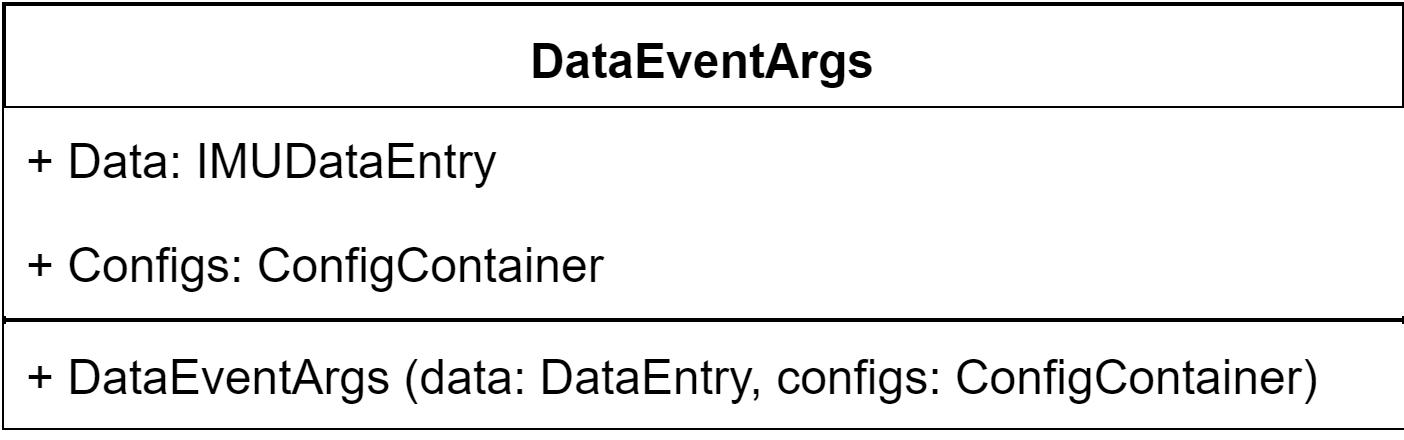
\includegraphics[width=\textwidth]{bilder/BibPackageKlassen/DataEventArgs.png}
\end{minipage}
\paragraph{Klassenbeschreibung:}
Enthält alle relevanten Informationen, die als Parameter mit dem Event IMUDataReceived gefeuert werden.

\paragraph{Attribute:}
\begin{itemize}
	\item[+] \textbf{Data: IMUDataEntry}\\Hier handelt es sich um die aktuelle und ausgewertete IMU Datenaufzeichnung.
	\item[+] \textbf{Configs: ConfigContainer}\\Hier werden die aktuellen Konfigurationen gespeichert.
\end{itemize}

\paragraph{Methoden:}
\begin{itemize}
	\item[+] \textbf{<<create>>DataEventArgs(connected: bool, deviceName: string): void}\\ Zusätzlicher Konstruktor um die Attribute setzten zu können
\end{itemize}






\subsection{Erweiterungsmodul}
\begin{center}
	\centering
	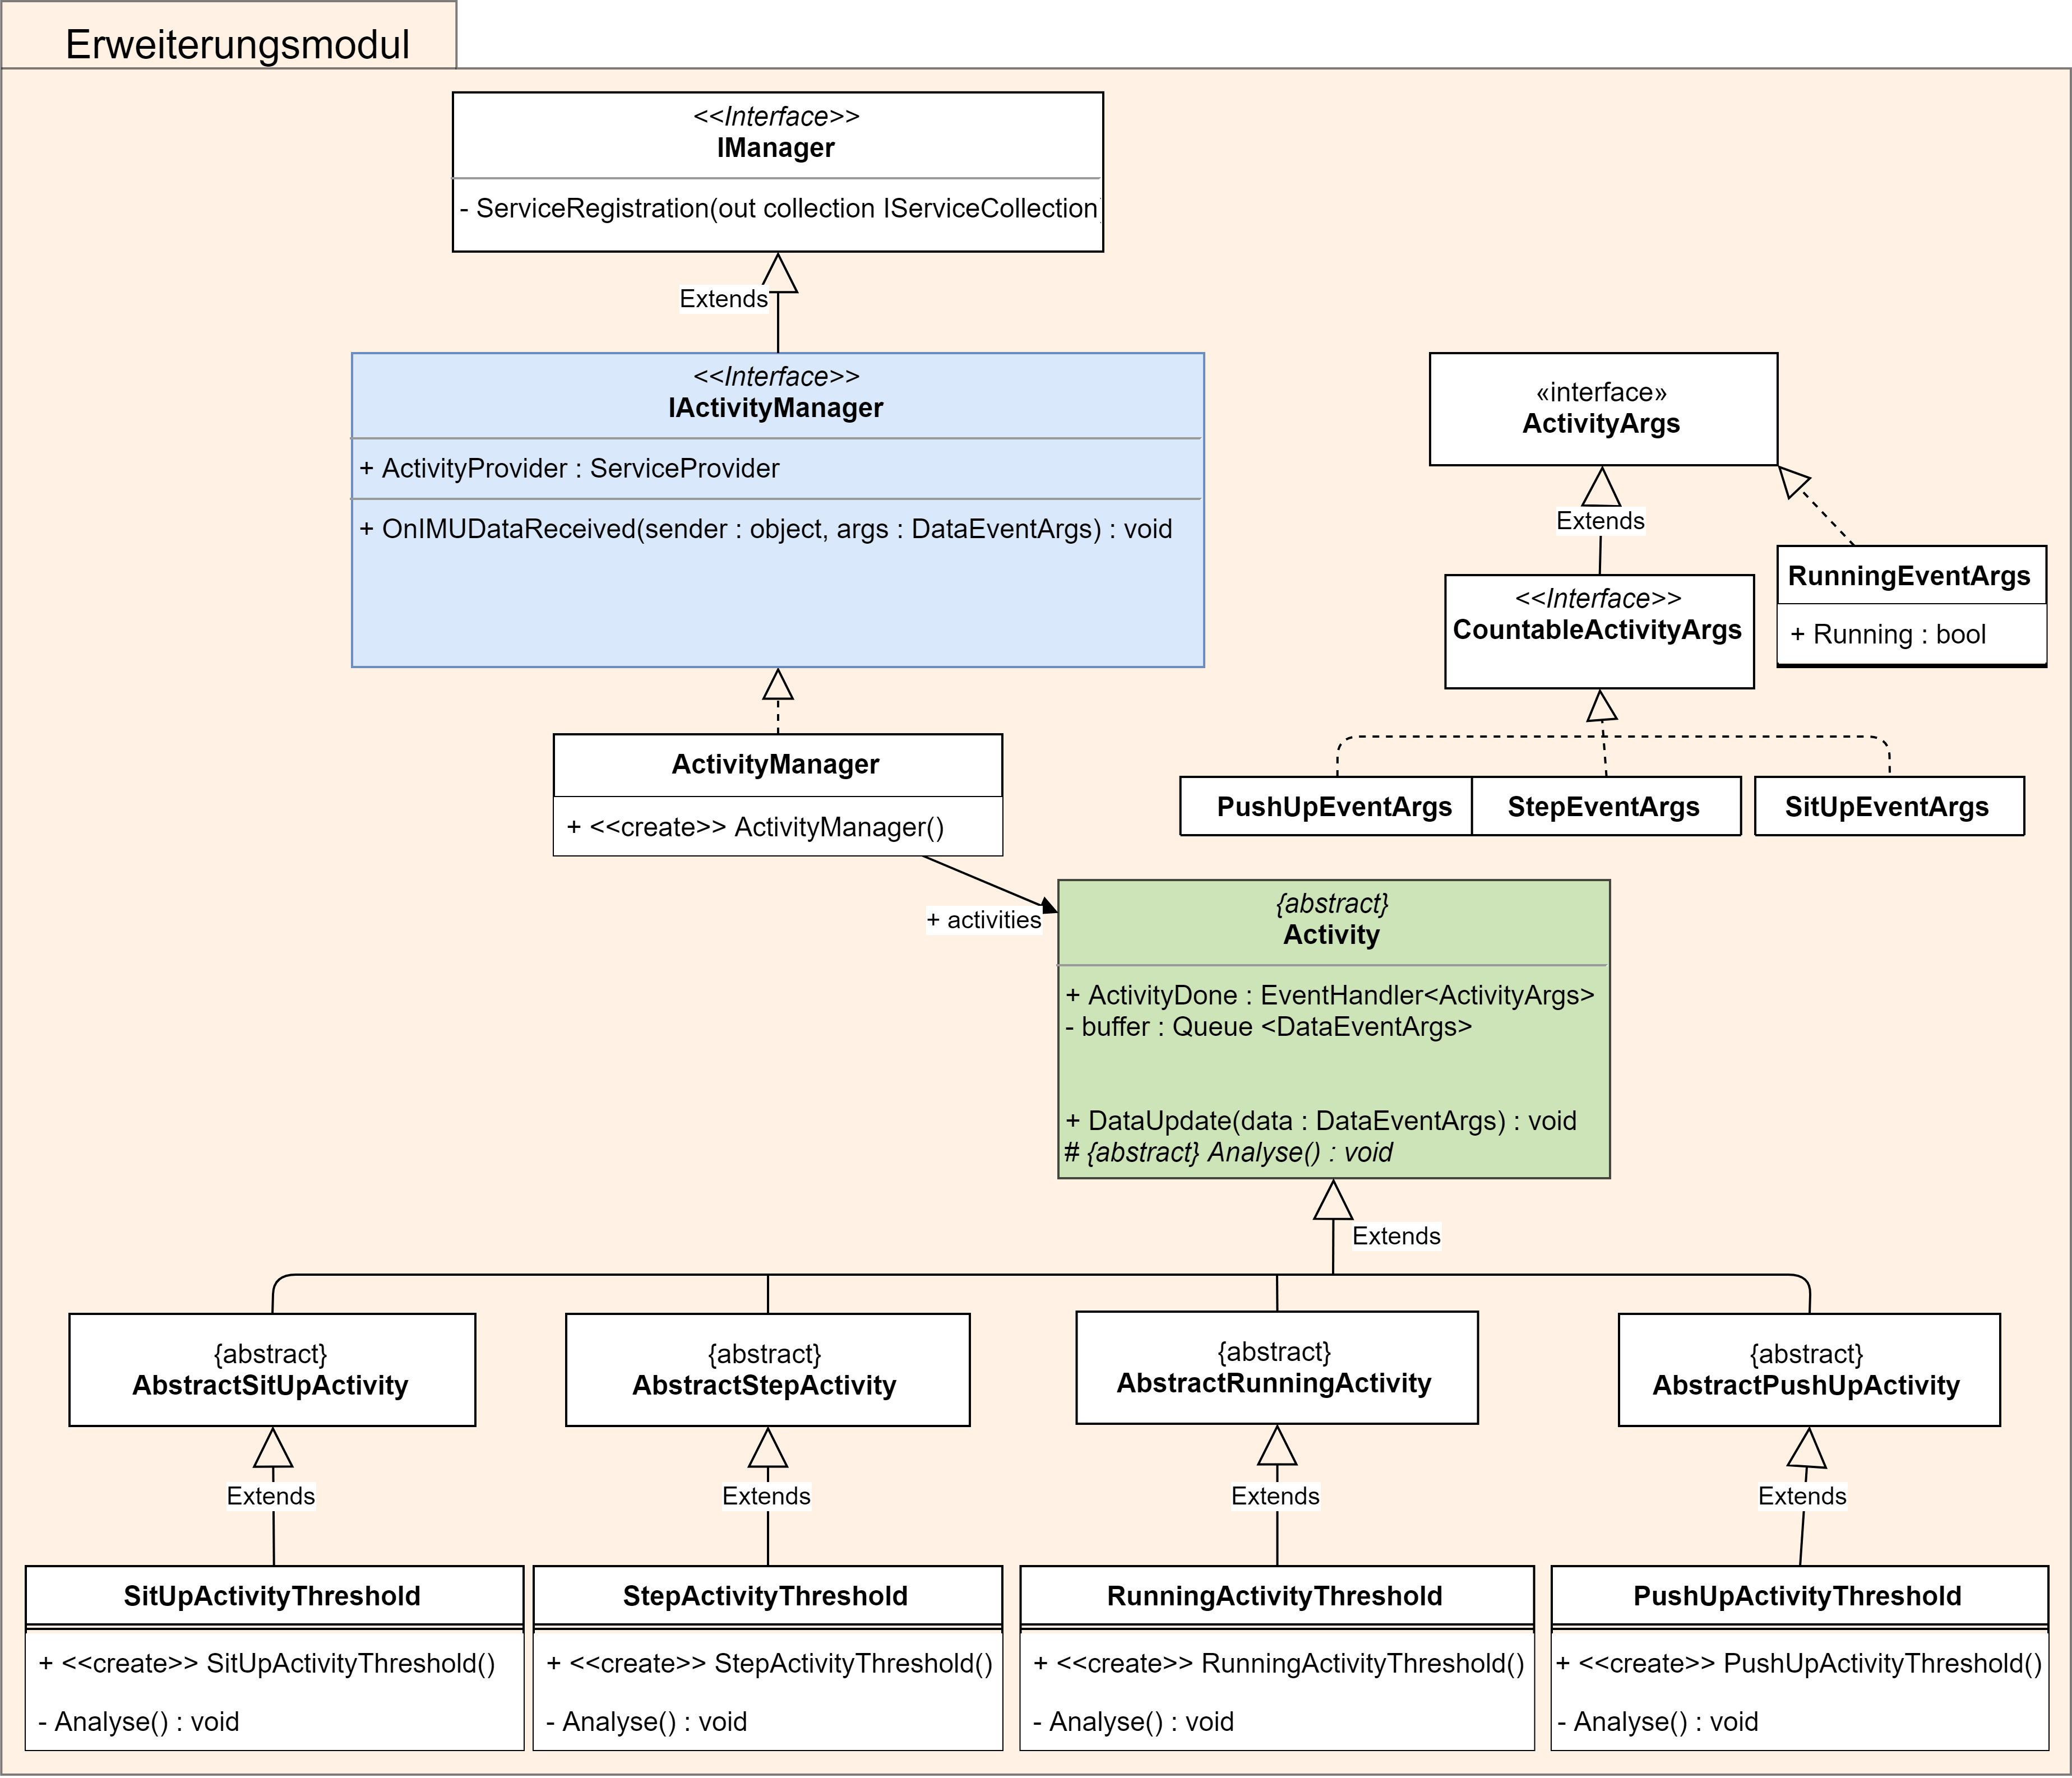
\includegraphics[width=15cm]{Diagramme/uebersicht/Erweiterungsmodul.png}
\end{center}

\begin{minipage}[b]{0.5\textwidth}
	\subsubsection{Interface IManager}
	
	\end{minipage}
	\begin{minipage}[c]{0.5\textwidth}
	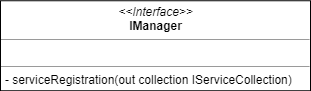
\includegraphics[width=\textwidth]{bilder/IManager.png}
\end{minipage}


	\paragraph{Schnittstellenbeschreibung:}
	Die Schnittstelle IManager definiert einen Service-Manager, welcher eine Menge an Services verwaltet. Dabei definiert die Schnittstelle die private Methode ServiceRegistration(out collection: IServiceCollection), um die Services bei der Erstanlegung zu registrieren. Die Schnittselle wird sowohl auf Erweiterungsmodul-Ebene als auch Model-Ebene implementiert (Klassen IActivityManager und ServiceManager). Die IServiceCollection ist aus der Erweiterung \Gls{DependencyInjection}.
	
	\paragraph{Methoden:}
	\begin{itemize}
		\item[$-$] \textbf{ServiceRegistration(out collection: IServiceCollection)}\\Legt eine IServiceCollection an und registriert dort die Services. Die IServiceCollection wird zurückgegeben.
	\end{itemize}
	
	
	\begin{minipage}[b]{0.5\textwidth}
		\subsubsection{Interface IActivityManager}
	\end{minipage}
	\begin{minipage}[c]{0.5\textwidth}
		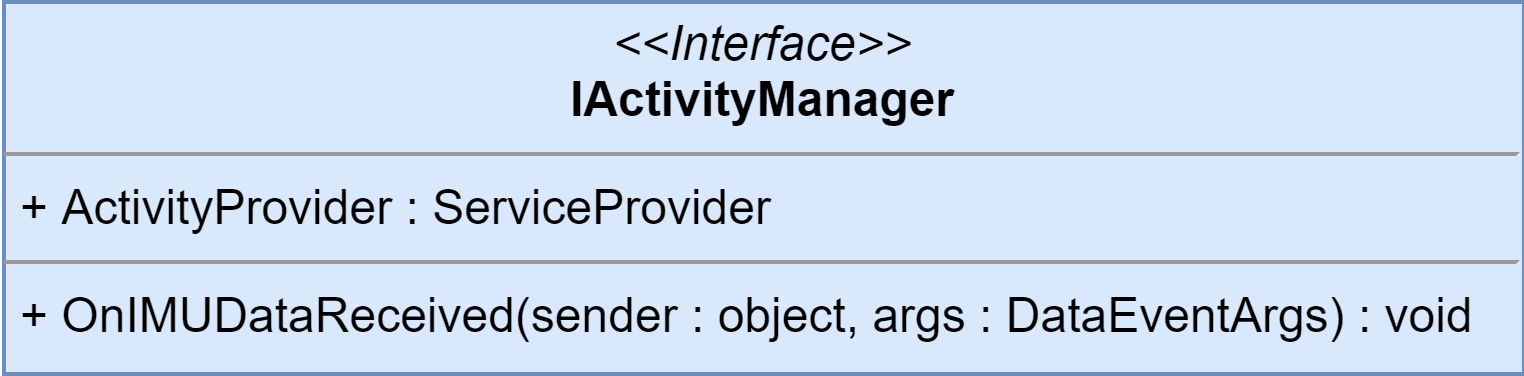
\includegraphics[width=\textwidth]{bilder/EMKlassen/IActivityManagerInterface.png}
	\end{minipage}
	
	\paragraph{Schnittstellenbeschreibung:}
	Die Schnittstelle IActivityManager erweitert die Schnittstelle IManager. Dabei definiert IActivityManager einen spezielleren Service-Manager. Dieser beinhaltet die Modi Services. Zudem definiert der IActivityManager die EventMethode OnIMUDataReceived(sender: object, args: DataEventArgs).\\
	Die Schnittstelle ist bei der Klasse ServiceManager als Service registriert und kann über diese von anderen Komponenten in der App angesprochen werden.
	
	\paragraph{Attribute:}
	\begin{itemize}
		\item[+] \textbf{ActivityProvider: ServiceProvider}\\Das Attribut ActivityProvider ist vom Typ ServiceProvider, eine Klasse aus der Erweiterung \Gls{DependencyInjection}. Dabei sind in dieser die registrierten Services gespeichert. Über die Methode GetService<T>() bekommt man eine konkrete Instanz des Services vom Typ T zurück. 
	\end{itemize}
	
	\paragraph{Methoden:}
	\begin{itemize}
		\item[$-$] \textbf{ServiceRegistration(out collection IServiceCollection)}\\Die Methode wird von der Schnittstelle IManager geerbt. Diese wird benötigt, um einen ServiceProvider zu erstellen (hier für das Attribut ActivityProvider).
		\item[+] \textbf{OnIMUDataReceived(sender: object, args: DataEventArgs): void}\\Die öffentliche Methode ist eine EventMethode, welche beim EventHandler IMUDataReceived der Klasse EarablesConnection registriert wird. Die konkreten Unterklassen müssen diese implementieren. 
	\end{itemize}
	
	
	
	\begin{minipage}[b]{0.6\textwidth}
		\subsubsection{Class ActivityManager}
	\end{minipage}
	\begin{minipage}[c]{0.4\textwidth}
		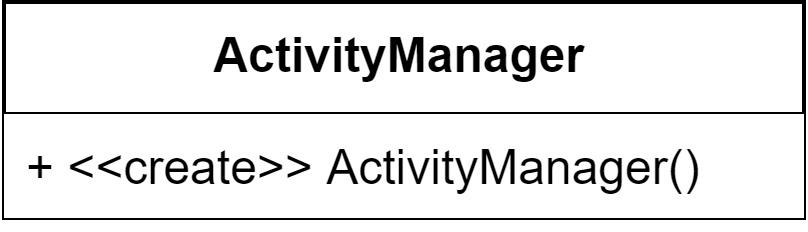
\includegraphics[width=\textwidth]{bilder/EMKlassen/ActivityMangerClass.png}
	\end{minipage}
	\paragraph{Klassenbeschreibung:}
	Die Klasse ActivityManager implementiert die Schnittstelle IActivityManager. Sie ist demnach ein Service-Manager und verwaltet die Activities (Vorgängeanalysen). Über sie können die ViewModels auf die Activities zugreifen.\\
	Der ActivityManager besitzt einen Service von den folgenden Typen: AbstractSitUpActivity, AbstractStepActivity, AbstractRunningActivity, AbstractPushUpActivity.\\
	Diese werden als Singletons gespeichert, was bedeutet, dass bei einem Aufruf von GetService<IT,T> immer die gleiche Instanz von T zurückgeliefert wird.
	
	\paragraph{Attribute:}
	\begin{itemize}
		\item[+] \textbf{activities: List<Activity>}\\Es wird eine Liste der registrierten Aktivitäten gespeichert. Bei einer Datenweitergabe muss somit nicht jedes mal vom ActivityProvider die Anfrage kommen, wer registriert ist. 
		\item[+] \textbf{ActivityProvider: ServiceProvider}\\Das Attribut beinhaltet die einzelnen Services mithilfe eines Dictionaries. Es wird in dem Konstruktor instanziiert.
	\end{itemize}
	\paragraph{Methoden:}
	\begin{itemize}
		\item[+] \textbf{<<create>> ActivityManager}\\Im Konstruktor registriert sich die Instanz der Klasse selbst bei dem EventHandler IMUDataReceived der Klasse EarablesConnection und ruft die private Methode ServiceRegistration(\dots) auf. Damit findet die Registrierung der Services und die Instanziierung des ActivityProviders statt.
		\item[$-$] \textbf{ServiceRegistration(out collection IServiceCollection): void}\\Private geerbte Methode der Schnittstelle IManager. Es wird eine ServiceCollection angelegt, bei der die Aktiväten registriert werden. Dies passiert mit der Methode collection.AddSingleton<IT,T>(). IT ist eine Oberklasse/Schnittstelle und T die konkrete Implementierung. IT ist in der Klasse ActivityManager immer eine Unterklasse vom Typ Activity (abstract).
		\item[+] \textbf{OnIMUDataReceived(sender: object, args: DataEventArgs): void}\\EventMethode, welche bei dem EventHandler IMUDataReceived der Klasse EarablesConnection registriert wird. Bei dem Aufrufen der Methode werden die Daten an die gespeicherten Aktivitäten weitergegeben. Das passiert per Push-Model (Observer-Muster), indem bei den Aktivitäten die Methode DataUpdate(data: DataEventArgs) aufgerufen wird. DataEventArgs sind dabei die neu erhaltenen Daten.\\

	\end{itemize}
	
	
	\begin{minipage}[b]{0.6\textwidth}
		\subsubsection{Class Activity}
	\end{minipage}
	\begin{minipage}[c]{0.4\textwidth}
		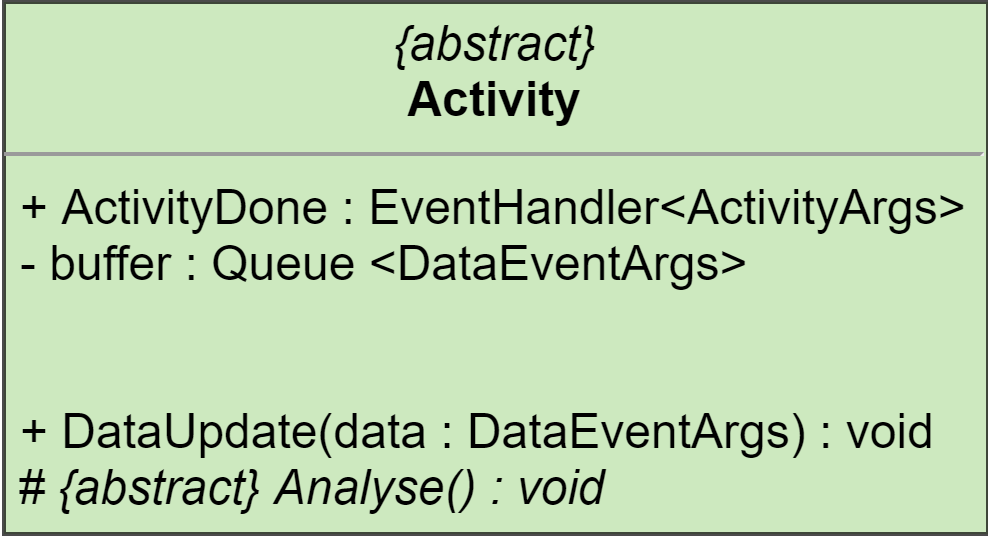
\includegraphics[width=\textwidth]{bilder/EMKlassen/ActivityClass.png}
	\end{minipage}
	
	\paragraph{Klassenbeschreibung}
	Activity ist eine abstrakte Klasse. Eine Activity ist im Wesentlichen ein Aktivitätserkennungsalgorithmus. Dabei wird die DataUpdate() Methode implementiert und den Unterklassen zu Verfügung gestellt. Der Algorithmus zur Aktivitätsanalyse (protected abstract void Analyse()) wird nur in konkreten Unterklassen implementiert. Dieser Entwurf entspricht dem Entwurfsmuster Schablone.
	
	\paragraph{Attribute:}
	\begin{itemize}
		\item[+] \textbf{ActivityDone: EventHandler<ActivityArgs>}\\Bei dem EventHandler können sich die ViewModel registrieren. Diese werden benachrichtigt, wenn eine Aktivität durchgeführt wurde (Schritt gelaufen, Liegestütze gemacht, etc.). Der EventHandler wird in der Methode Analyse() aufgerufen. Als Argument bei dem Eventwurf wird ein Objekt des Types ActivityArgs übergeben.
		\item [$-$] \textbf{buffer: Queue <DataEventArgs>}\\In der Queue werden die ankommenden Dateneinträge gespeichert. Diese werden nacheinander von dem Algorithmus in Analyse() verwendet. 
	\end{itemize}
	\paragraph{Methoden:}
	\begin{itemize}
		\item[+] \textbf{DataUpdate(data: DataEventArgs): void}\\Mit dieser Methode bekommt die Aktivität die neuen Dateneinträge. Dabei ruft die Klasse ActivityManager die Methode auf, wenn sie die neuen Daten bekommt. In dieser Methode wird geschaut, ob sich ein Event bei dem EventHandler ActivityDone registriert hat. Falls ja, wird der Datensatz dem buffer hinzugefügt, und der Algorithmus gestartet. Falls nicht, wird der Datensatz ignoriert.
		\item[\#] \textbf{abstract Analyse(): void}\\Der Algorithmus der Aktivitätserkennung wird in dieser Methode ausgeführt. Dabei ist dieser in den Unterklassen implementiert. Er beurteilt nur mithilfe der gesammelten Gyroskop- und Accelerometerdaten, ob das (der Activity entsprechende) Ereignis eingetroffen ist. In diesem Fall feuert er ein Event über den ActivityDone EventHandler. 
	\end{itemize}
	
	\begin{minipage}[b]{0.65\textwidth}
		\subsubsection{Abstract Class AbstractStepActivity}
	\end{minipage}
	\begin{minipage}[c]{0.35\textwidth}
		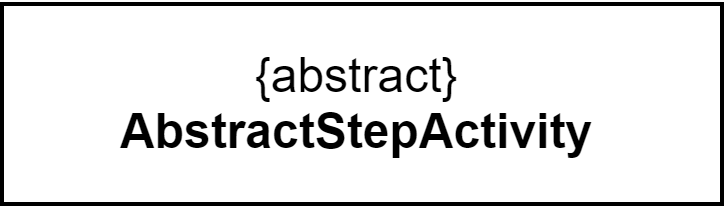
\includegraphics[width=\textwidth]{bilder/EMKlassen/AbstractStepActivityClass.png}
	\end{minipage}
	\paragraph{Klassenbeschreibung:}
	Diese Klasse dient nur zur Gewährleistung der Modularität für den ServiceManager. Alle Kinder dieser Klasse sind verschiedene Algorithmen zur Schritterkennung.\\ Es soll immer ein Event gefeuert werden, wenn ein Schritt getätigt wurde.\\
	\newline
	\begin{minipage}[b]{0.6\textwidth}
		\subsubsection{Class StepActivityThreshold}
		\end{minipage}
		\begin{minipage}[c]{0.4\textwidth}
			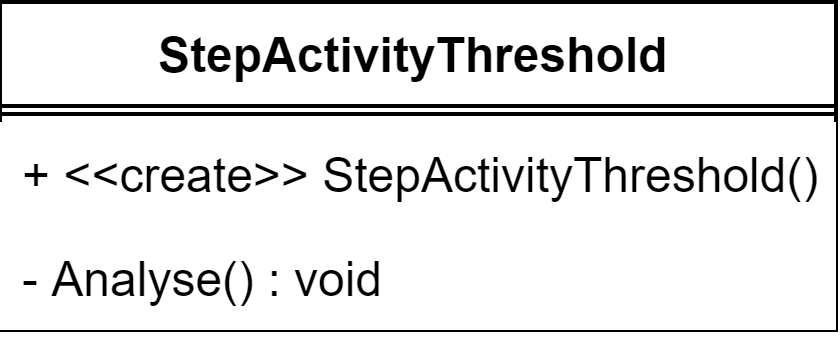
\includegraphics[width=\textwidth]{bilder/EMKlassen/StepActivityThresholdClass.png}
		\end{minipage}
	\paragraph{Klassenbeschreibung:}
	Diese Klasse beinhaltet den Threshold-Algorithmus für die Erkennung, wann ein Schritt getätigt wurde. Es handelt sich hierbei um eine Kindklasse der abstrakten Klasse AbstractStepActivity. 
	\paragraph{Methoden:}
	\begin{itemize}
		\item [+]\textbf{<<create>> StepActivityThreshold(): void}\\Konstruktor der KlasseStepActivityThreshold. Dabei wird der EventHandler ActivityDone initialisiert. 
		\item [$-$]\textbf{Analyse(): void}\\ Implementierung der Analyse für die Schritterkennung. Dabei basiert diese auf dem Threshold Ansatz.\\
	\end{itemize}
	
	
	
	\begin{minipage}[b]{0.65\textwidth}
		\subsubsection{Abstract Class AbstractRunningActivity}
		\end{minipage}
		\begin{minipage}[c]{0.35\textwidth}
			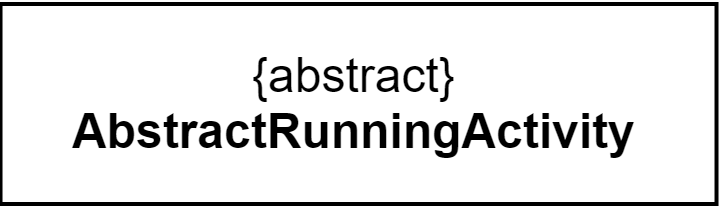
\includegraphics[width=\textwidth]{bilder/EMKlassen/AbstractRunningActivityClass.png}
		\end{minipage}
	\paragraph{Klassenbeschreibung:}
	Diese Klasse dient nur zur Gewährleistung der Modularität für den ServiceManager. Alle Kinder dieser Klasse sind verschiedene Algorithmen zur Erkennung, ob der Nutzer läuft oder steht.\\ Es wird immer dann ein Event gefeuert, wenn sich dieser Status ändert.\\
	\newline
	\begin{minipage}[b]{0.6\textwidth}
		\subsubsection{Class RunningActivityThreshold}
		\end{minipage}
		\begin{minipage}[c]{0.4\textwidth}
			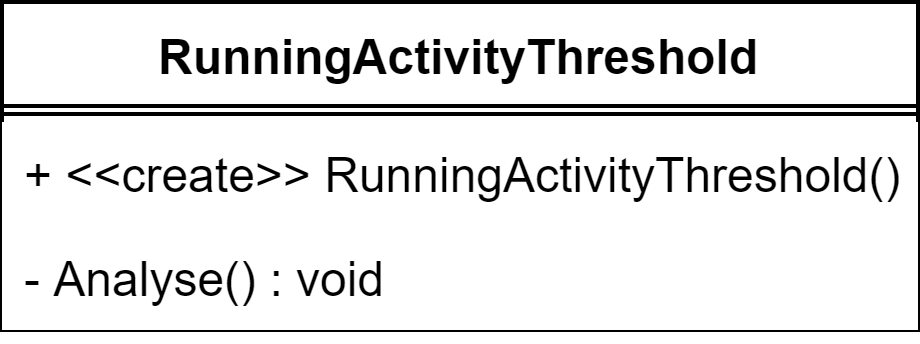
\includegraphics[width=\textwidth]{bilder/EMKlassen/RunningActivityThresholdClass.png}
		\end{minipage}
		
	\paragraph{Klassenbeschreibung:}
	Diese Klasse beinhaltet den Threshold-Algorithmus für die Erkennung, ob der Nutzer läuft oder steht. Es wird nur analysiert, falls sich mindestens ein Event bei dem geerbten EventHandler ActivityDone registriert hat.
	\paragraph{Methoden:}
	\begin{itemize}
		\item [+]\textbf{<<create>> SitUpActivityThreshold(): void}\\Konstruktor der Klasse RunningActivityThreshold. In diesem wird der EventHandler erstellt.
		\item [$-$]\textbf{Analyse(): void}\\Implementierung der Analyse, ob der Nutzer läuft oder steht. Der EventHandler ActivityDone ruft die Events auf, falls sich der Laufstatus ändert. Das bedeutet, wenn der Nutzer anfängt zu laufen, oder aufhört. 
		\newline	
\end{itemize}
	
	\begin{minipage}[b]{0.65\textwidth}
		\subsubsection{Abstract Class AbstractPushUpActivity}
		\end{minipage}
		\begin{minipage}[c]{0.35\textwidth}
			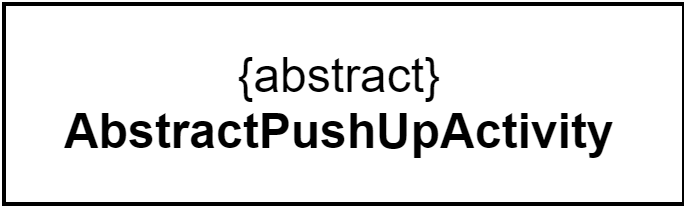
\includegraphics[width=\textwidth]{bilder/EMKlassen/AbstractPushUpActivityClass.png}
		\end{minipage}
		
	\paragraph{Klassenbeschreibung:}
	Diese Klasse dient nur zur Gewährleistung der Modularität für den ServiceManager. Alle Kinder dieser Klasse sind verschiedene Algorithmen zur Erkennung von Push-ups.\\ Es soll immer ein Event gefeuert werden, wenn eine Liegestütze erkannt wurde.\\
	\newline
	\begin{minipage}[b]{0.6\textwidth}
		\subsubsection{Class PushUpActivityThreshold}
		\end{minipage}
		\begin{minipage}[c]{0.4\textwidth}
			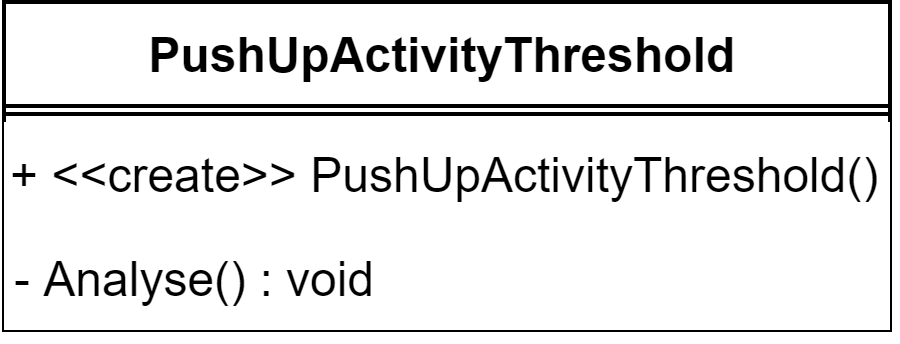
\includegraphics[width=\textwidth]{bilder/EMKlassen/PushUpActivityThresholdClass.png}
		\end{minipage}
	\paragraph{Klassenbeschreibung:}
	Diese Klasse beinhaltet den Threshold-Algorithmus für die Erkennung von Push-ups. Es wird nur analysiert, falls sich mindestens ein Event bei dem geerbten EventHandler ActivityDone registriert hat.
	\paragraph{Methoden:}
	\begin{itemize}
		\item [+]\textbf{<<create>> PushUpActivityThreshold(): void}\\Konstruktor der Klasse PushUpActivityThreshold(). In diesem wird der EventHandler ActivityDone instanziiert. 
		\item [$-$]\textbf{Analyse(): void}\\Implementierung der Analyse für die Sit-Up-Erkennung. Dabei werden die Daten aus der Queue Buffer benutzt. Der EventHandler ruft die Events auf, wenn eine Liegestütze gemacht wurde.\\
		\newline	
\end{itemize}

	\begin{minipage}[b]{0.65\textwidth}
		\subsubsection{Abstract Class AbstractSitUpActivity}
		\end{minipage}
		\begin{minipage}[c]{0.35\textwidth}
			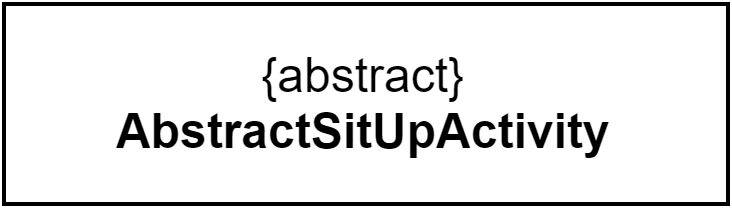
\includegraphics[width=\textwidth]{bilder/EMKlassen/AbstractSitUpActivityClass.png}
		\end{minipage}
		
	\paragraph{Klassenbeschreibung:}
	Diese Klasse dient nur zur Gewährleistung der Modularität für den ServiceManager. Alle Kinder dieser Klasse sind verschiedene Algorithmen zur Erkennung von Sit-ups.\\ Es soll nach jedem erkannten Sit-up ein Event gefeuert werden.\\
	\newline
	\begin{minipage}[b]{0.6\textwidth}
		\subsubsection{Class SitUpActitvityThreshold}
		\end{minipage}
		\begin{minipage}[c]{0.4\textwidth}
			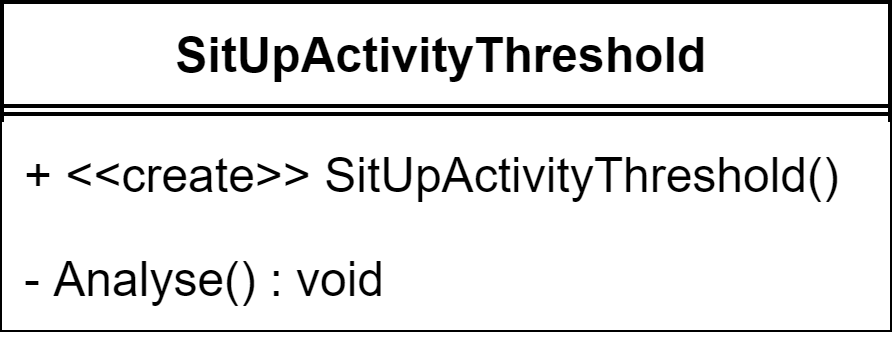
\includegraphics[width=\textwidth]{bilder/EMKlassen/SitUpActivityThresholdClass.png}
		\end{minipage}
		
	\paragraph{Klassenbeschreibung:}
	Diese Klasse beinhaltet den Threshold-Algorithmus für die Erkennung von Sit-ups. Hier wird basierend auf den Daten der Earables der Algorithmus in der Methode Analyse() ausgeführt.
	\paragraph{Methoden:}
	\begin{itemize}
		\item [+]\textbf{<<create>> SitUpActivityThreshold(): void}\\Konstruktor der Klasse SitUpActivityThreshold. In dieser wird der EventHandler instanziiert. 
		\item [$-$]\textbf{Analyse(): void}\\ Implementierung der Analyse des Ereignisses. Dabei basiert dieser auf einem Threshold Ansatz. Diese wird nur ausgeführt, falls sich ein Event bei ActivityDone registriert hat.
	\end{itemize}
		
	
	\begin{minipage}[b]{0.7\textwidth}
		\subsubsection{Interface ActivityArgs}
		\end{minipage}
		\begin{minipage}[c]{0.3\textwidth}
			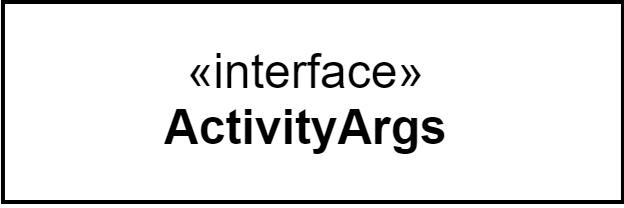
\includegraphics[width=\textwidth]{bilder/EMKlassen/ActivityArgsInterface.png}
		\end{minipage}
		
	\paragraph{Schnittstellenbeschreibung:}
	ActivityArgs werden beim Feuern eines Events mit dem Event übergeben. Das erkannte Ereignis kann durch die ActivityArgs genauer beschrieben werden.\\
	
	\begin{minipage}[b]{0.8\textwidth}
		\subsubsection{Class RunningEventArgs}
		\end{minipage}
		\begin{minipage}[c]{0.2\textwidth}
			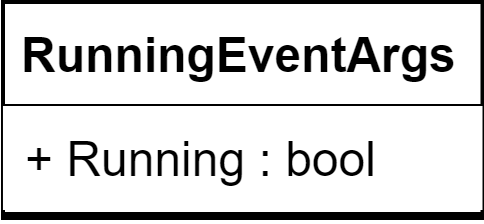
\includegraphics[width=\textwidth]{bilder/EMKlassen/RunningEventArgsClass.png}
		\end{minipage}
		
	\paragraph{Klassenbeschreibung:}
	Ein Event der RunningActivityThreshold sagt entweder aus, dass der Nutzer stoppt, oder, dass er zu laufen beginnt. Beim Werfen dessen wird eine Instanz dieser Klasse übergeben.
	\paragraph{Attribute:}
	\begin{itemize}
		\item[+] \textbf{Running: bool}\\ Dieses Attribut ist genau dann auf wahr (true) gesetzt, wenn der Nutzer zu laufen beginnt; falsch (false), wenn der Nutzer stoppt.\\
	\end{itemize} 

	\begin{minipage}[b]{0.8\textwidth}
		\subsubsection{Interface CountableActivityArgs}
	\end{minipage}
	\begin{minipage}[c]{0.2\textwidth}
		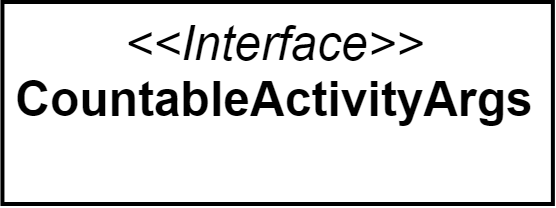
\includegraphics[width=\textwidth]{bilder/EMKlassen/CountableActivityArgsInterface.png}
	\end{minipage}

	\paragraph{Schnittstellenbeschreibung:}
	Diese Schnittstelle spezifiziert alle EventArgs bei Aktivitäten, bei denen gezählt werden kann. Auch wenn momentan keine weiteren EventArgs verwendet werden, stärkt diese Struktur die Erweiterbarkeit und Übersichtlichkeit. Falls für zählbare Aktivitäten weitere Argumente angegeben werden sollen, kann dies gebündelt geschehen.\\
	\newline
	
	
	\begin{minipage}[b]{0.8\textwidth}
		\subsubsection{Class PushUpEventArgs}
		\end{minipage}
		\begin{minipage}[c]{0.2\textwidth}
			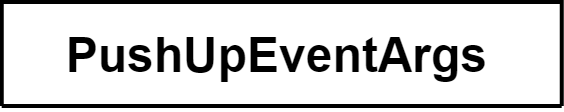
\includegraphics[width=\textwidth]{bilder/EMKlassen/PushUpEventArgsClass.png}
		\end{minipage}
	\paragraph{Klassenbeschreibung:}
	Aktuell gibt es keine relevanten Argumente bei Push-ups. Dies kann bei einem anderen Algorithmus-Ansatz (siehe Aktivität) der Fall sein. Bei Bedarf kann man der Klasse weitere Attribute geben.\\
	
	\begin{minipage}[b]{0.8\textwidth}
		\subsubsection{Class StepEventArgs}
		\end{minipage}
		\begin{minipage}[c]{0.2\textwidth}
			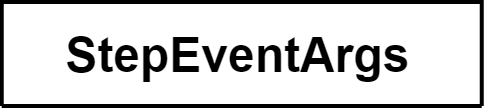
\includegraphics[width=\textwidth]{bilder/EMKlassen/StepEventArgsClass.png}
		\end{minipage}
	\paragraph{Klassenbeschreibung:}
	Aktuell gibt es keine relevanten Argumente bei der Schritterkennung. Dies kann bei einem anderen Algorithmus-Ansatz (siehe Aktivität) der Fall sein. Bei Bedarf kann man der Klasse weitere Attribute geben.\\
	\newline
	\begin{minipage}[b]{0.8\textwidth}
		\subsubsection{Class SitUpEventArgs}
		\end{minipage}
		\begin{minipage}[c]{0.2\textwidth}
			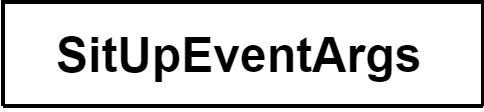
\includegraphics[width=\textwidth]{bilder/EMKlassen/SitUpEventArgsClass.png}
		\end{minipage}
	\paragraph{Klassenbeschreibung:}
	Aktuell gibt es keine relevanten Argumente bei Sit-ups. Dies kann bei einem anderen Algorithmus-Ansatz (siehe Aktivität) der Fall sein. Bei Bedarf kann man der Klasse weitere Attribute geben.\\
	\newline
	

\begin{minipage}[b]{0.6\textwidth}
	\subsection{Class ServiceManager}
\end{minipage}
\begin{minipage}[c]{0.4\textwidth}
	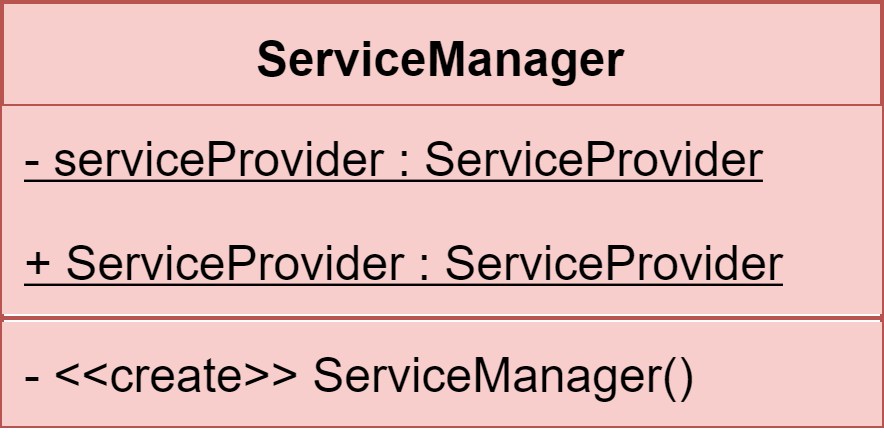
\includegraphics[width=\textwidth]{bilder/EMKlassen/ServiceManagerClass.png}
\end{minipage}
	\paragraph{Klassenbeschreibung:}
	Der ServiceManager verwaltet alle Services des Models mithilfe eines statischen Serviceproviders. Dies wird von anderen Services des Models, sowie von dem ViewModel benutzt. Er dient zur Delegierung der Services.\\ 
	Dabei implementiert der ServiceManager das Interface IManager.
	Von diesem bekommt er die Methode serviceRegistration() übergeben.
	Der ServiceManager speichert die Services als Referenzen und achtet, dass diese ein Singleton sind. (Es existiert immer nur eine Instanz des Services).
	Er implementiert das Singleton Muster indem der Serviceprovider nur einmal instanziiert wird.
	
	\paragraph{Attribute:}
	\begin{itemize}
		\item[$-$] \textbf{static serviceProvider: ServiceProvider}\\Eine private Instanz vom Typ ServiceProvider. Beinhaltet die Referenzen auf die Services und verwaltet die Zugriffe darauf. Dies geschieht per GetService<T>.
		\item[+] \textbf{static ServiceProvider: ServiceProvider}\\Property für die Instanz serviceProvider. Reguliert, dass der serviceProvider nur einmal existiert. (Singleton-Entwurfsmuster)

	\end{itemize}
	\paragraph{Methoden:}
	\begin{itemize}
		\item[$-$] \textbf{<<create>> ServiceProvider()}\\Privater Konstruktor, da es sich um eine statische Klasse handelt ohne Instanzattribute.
		\item[$-$] \textbf{serviceRegistration()}\\ Zur erstmaligen Registrierung der Services mit einer IServiceCollection und zur Erstellung des Attributs serviceProvider.\\
	\end{itemize}
		
		
\subsection{Settings Service}
\begin{minipage}[b]{0.6\textwidth}
\subsubsection{Interface ISettingsService}
\end{minipage}
\begin{minipage}[c]{0.4\textwidth}
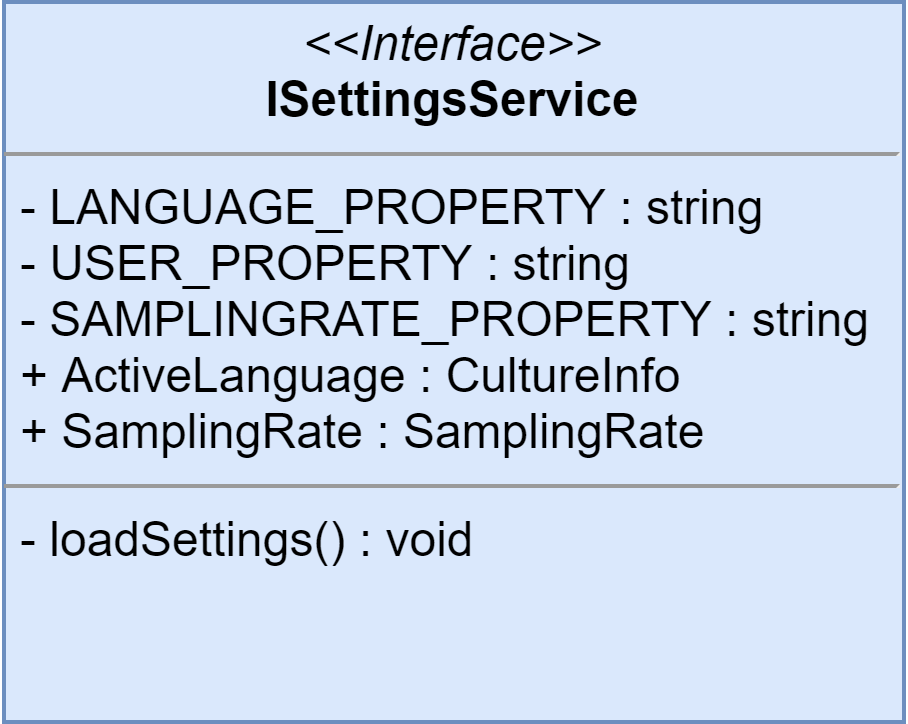
\includegraphics[width=\textwidth]{bilder/EMKlassen/ISettingsServiceInterface.png}
\end{minipage}



	\paragraph{Schnittstellenbeschreibung:}
	ISettingsService bietet eine Schnittstelle für die Einstellungen der App. Sie implementiert die Einstellungen und hält die aktuellen Instanzen dieser als Attribute.
	\paragraph{Attribute:}
	\begin{itemize}
		\item[+] \textbf{ActiveLanguage: CultureInfo}\\Die aktuelle Sprache der App (Deutsch oder Englisch)\\
		\item[+] \textbf{SamplingRate: SamplingRate}\\Die aktuelle Samplingrate der \Gls{Earables} \\ 
		\item[+] \textbf{MyUser: User}\\Der aktuelle User, der die App benutzt.\\
	\end{itemize}


\begin{minipage}[b]{0.6\textwidth}
	\subsubsection{Class SettingsService}
\end{minipage}
\begin{minipage}[c]{0.4\textwidth}
	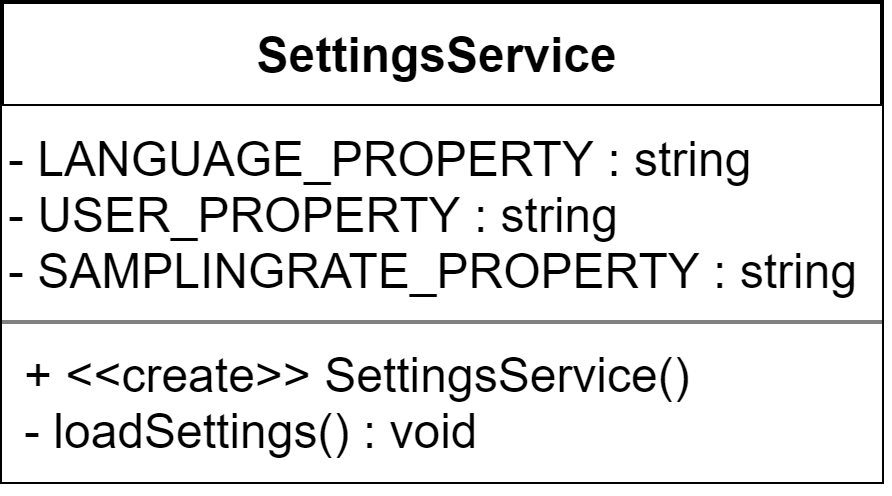
\includegraphics[width=\textwidth]{bilder/EMKlassen/SettingsServiceClass.png}
\end{minipage}
	\paragraph{Klassenbeschreibung}
	Die Klasse SettingsService implementiert die Schnittstelle ISettingsService. Zur Speicherung der Einstellungen wird die Klasse App.Current.Properties verwendet.
	Dabei wird immer sofort nach einer Änderung die neue Einstellung gespeichert und nicht erst beim Beenden der Sitzung.

	Das wird dadurch sicher gestellt, dass die Attribute als Properties gespeichert sind, welche beim Setzen (set) stets 'App.Current.Properties[Schlüssel] = value;' benutzen.
	\paragraph{Attribute:}
	\begin{itemize}
		\item[+] \textbf{ActiveLanguage: CultureInfo}\\Die aktuelle Sprache der App (Deutsch oder Englisch). Attribut aus dem Interface ISettingsService\\
		\item[+] \textbf{SamplingRate: SamplingRate}\\Die aktuelle Samplingrate der \Gls{Earables}\\ 
		\item[$-$] \textbf{LANGUAGE\_PROPERTY: string}\\Konstanter Bezeichner für die Einstellung der Sprache. Ist der Bezeichner für die Sprache im Dictionary in App.Properties.\\
		\item[$-$] \textbf{USER\_PROPERTY: string}\\Konstanter Bezeichner für die Einstellung des Nutzers.Ist der Bezeichner für den User im Dictionary in App.Properties.\\
		\item[$-$] \textbf{SAMPLINGRATE\_PROPERTY: string}\\Konstanter Bezeichner für die Einstellung der Samplingrate. Ist der Bezeichner für die SamplingRate im Dictionary in App.Properties. \\
	\end{itemize}

  \paragraph{Methoden:}
	\begin{itemize}
		\item[+] \textbf{<<create>> SettingsService}\\Konstruktor für die Klasse SettingsService. Dabei wird er als Service vom ServiceManager verwaltet, demnach existiert er nur als Singleton.\\
		\item[$-$] \textbf{LoadSettings():void}\\Lädt alle Settings aus den Einstellungen in die Attribute. Wird im Konstruktor aufgerufen. (Beim Start)\\
		\newline
	\end{itemize}



\begin{minipage}[b]{0.6\textwidth}
	\subsubsection{Class User}
\end{minipage}
\begin{minipage}[c]{0.4\textwidth}
	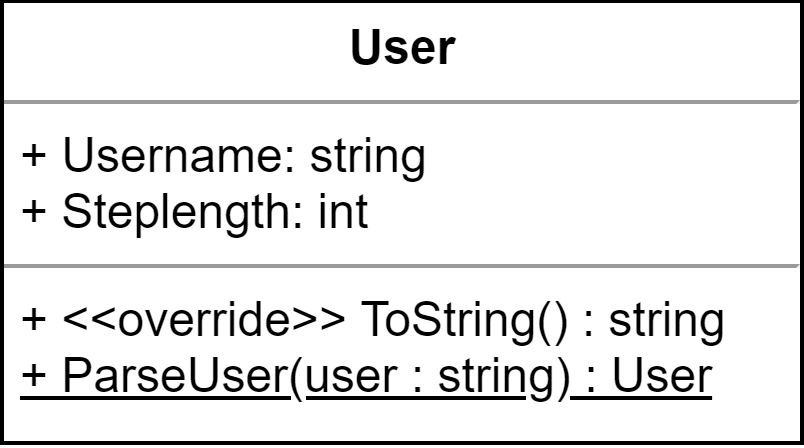
\includegraphics[width=\textwidth]{bilder/EMKlassen/UserClass.png}
\end{minipage}

	\paragraph{Klassenbeschreibung:}
	Die User-Klasse spezifiziert den Nutzer, der die App gerade verwendet. In dieser werden Attribute gespeichert, welche von Nutzer zu Nutzer anders sind. Falls der Nutzer sein Konto noch nicht eingerichtet hat, wird ein Standardnutzer geladen.\\
	\paragraph{Attribute:}
	\begin{itemize}
		\item[+] \textbf{Username: string}\\Der Name des Nutzers. Dabei ist der Standardname 'Nutzer'\\
		\item[+] \textbf{Steplength: int}\\Die durchschnittliche Schrittlänge des Nutzers in Zentimeter Die Standardlänge beträgt 70cm.\\

	\end{itemize}
	\paragraph{Methoden:}
	\begin{itemize}
		\item[+] \textbf{<<override>> ToString(): string}\\Wandelt das Objekt in einen string um. Damit ist geregelt, dass der User als string in den App.Current.Properties gespeichert werden kann. Er wird in ein \Gls{CSV}-Format umgewandelt.\\
		Beispiel: ``Alice van Bob,80'' ist die string-Repräsentation des Users mit Username ``Alice van Bob'' und Steplength 80.\\
		\item[+] \textbf{static ParseUser(user: string): User}\\Statische Methode, welche einen \Gls{CSV}-String wieder in  ein Objekt umwandelt. Das Format ist in der ToString() Methode spezialisiert. Falls der übergeben string nicht dem Format entspricht, so wird 'null' zurückgegeben.\\
	\end{itemize}

	\begin{minipage}[b]{0.6\textwidth}
		\subsubsection{Enumeration SamplingRate}
	\end{minipage}
	\begin{minipage}[c]{0.0\textwidth}
		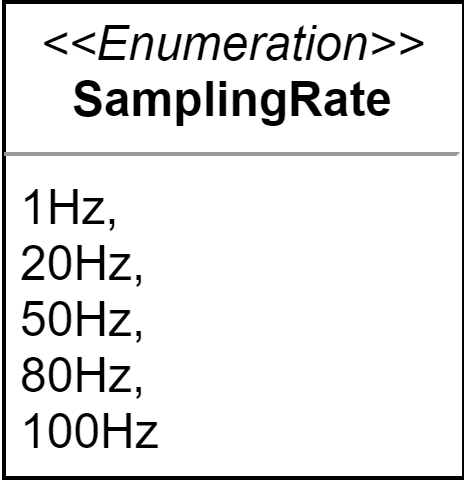
\includegraphics[width=\textwidth]{bilder/EMKlassen/SamplingRateEnum.png}
	\end{minipage}
	\paragraph{Enumerationbeschreibung}
	Das Enum SamplingRate gibt dem User die Auswahl die SamplingRate (Anzahl der Stichproben). Dazu gibt es mehrere Einstellungsraten von 1-100 Hz (Herz). Diese aktuelle SamplingRate wird in den App.Properties gespeichert. Dies wird von der Klasse SettingsService verwaltet. 
	Bei der Änderung wird die Samplerate von der ViewModel-Ebene aus der Bibliothek geschickt und auf den \Gls{Earables} gesetzt.

	
	\paragraph{Werte:}
	\begin{itemize}
		\item \textbf{1 Hz}\\SampleRate mit einem Herz. Eine Stichprobe pro Sekunde
		\item \textbf{20 Hz}\\SampleRate mit zwanzig Herz. 20 Stichproben pro Sekunde
		\item \textbf{50 Hz}\\SampleRate mit fünfzig Herz. 50 Stichproben pro Sekunde
		\item \textbf{80 Hz}\\SampleRate mit achtzig Herz. 80 Stichproben pro Sekunde
		\item \textbf{100 Hz}\\SampleRate mit einhundert Herz. 100 Stichproben pro Sekunde
	\end{itemize}
	
	
	
	
	
	
	
\subsection{Datenbank Service}
\subsubsection{Interface IDataBaseConnection}
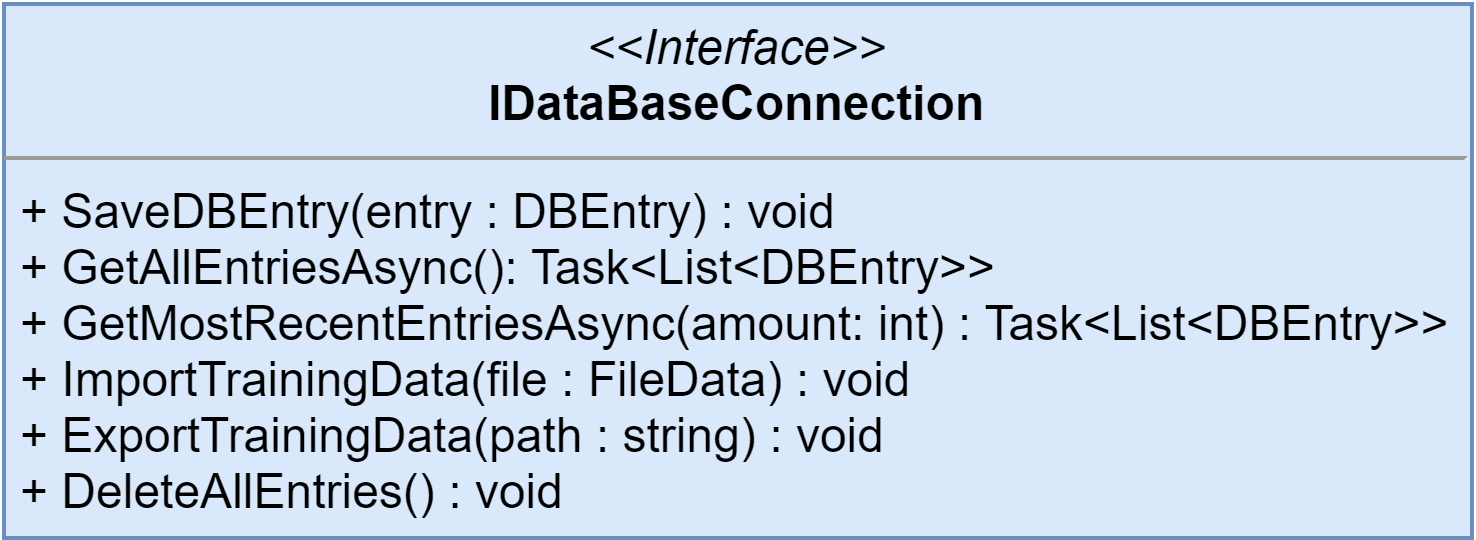
\includegraphics{bilder/EMKlassen/IDataBaseConnectionInterface.png}
	\paragraph{Schnittstellenbeschreibung}
	Das Interface IDataBaseConnection ist ein Service, welcher vom ServiceManager verwaltet wird. Dieser regelt Speicherung der Trainingsdaten mittels einer \gls{Datenbank}. Zudem implementiert er das Importieren und Exportieren von den Trainingsdaten.
	Die Datenbankeinträge sind Instanzen der Klasse DBEntry. 
	
	\paragraph{Methoden:}
	\begin{itemize}
		\item[+] \textbf{SaveDBEntry(entry: DBEntry): void}\\Speichert ein Datenbankeintrag in der \gls{Datenbank}. Falls schon ein Eintrag zu dem Datum existiert, wird dieser aktualisiert\\

		\item[+] \textbf{GetAllEntriesAsync(): Task<List<DBEntry> >}\\Liefert einem alle Einträge der Datenbank in Form von einer Liste mit DBEntry.\\ 
		\item[+] \textbf{GetMostRecentEntriesAsync(amount : int): void}\\Liefert  die letzten 'amount' Einträge der Datenbank in Form einer Liste mit DBEntry zurück.\\
		\item[+] \textbf{ImportTrainingData(file: FileData): void}\\Liest aus der angegebenen \gls{CSV}-Datei die DBEntries raus und speichert sie in der \gls{Datenbank}.\\
		\item[+] \textbf{ExportTrainingData(path: string): void}\\Exportiert die Trainingsdaten aus der \gls{Datenbank} in einer \gls{CSV}-Datei in den Ordner bei path. \\
	\end{itemize}
\begin{minipage}[b]{0.6\textwidth}
	\subsubsection{Class DataBaseConnection}
\end{minipage}
\begin{minipage}[c]{0.4\textwidth}
	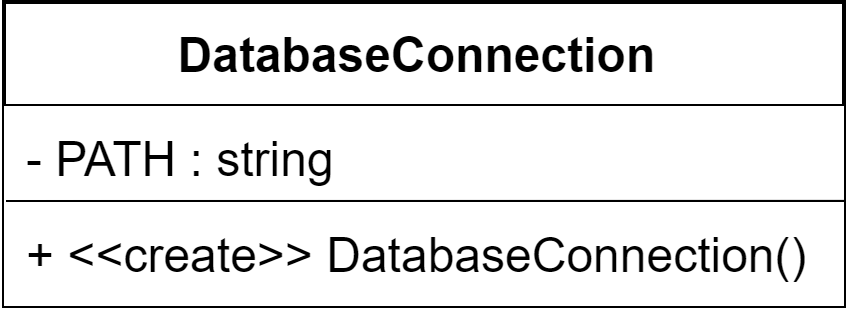
\includegraphics[width=\textwidth]{bilder/EMKlassen/DataBaseConnectionClass.png}
\end{minipage}
	\paragraph{Klassenbeschreibung}
	Die Klasse DataBaseConnection implementiert die Schnittstelle IDataBaseConnection. Sie kümmert sich um die Speicherung und Verwaltung der Trainingsdaten. Dabei benutzt die DataBaseConnection die \gls{Datenbank} von SQLite. Es werden Objekte von der Klasse DBEntry gespeichert. 
	
	\paragraph{Attribute:}
	\begin{itemize}
		\item[$-$] \textbf{const PATH: string}\\Der Pfad, an dem die Datenbank gespeichert ist. Dabei ist dieser Pfad konstant und kann nicht geändert werden.
	\end{itemize}
	\paragraph{Methoden:}
	\begin{itemize}
		\item[+] \textbf{<<create>> DatabaseConnection}\\Konstruktor für die Klasse DatabaseConnection. Es wird eine Instanz SQLiteAsyncConnection und eine Tabelle erstellt. Diese besteht aus zwei Spalten: Das Datum(Primary Key) als Datetype und den Inhalt als string.
		\item[+] \textbf{SaveDBEntry(entry: DBEntry): void}\\Speichert ein Datenbankeintrag in der \gls{Datenbank}. Falls schon ein Eintrag zu dem Datum existiert, wird dieser aktualisiert, indem die Werte addiert werden.\\
		\item[+] \textbf{GetAllEntriesAsync(): Task<List<DBEntry>>}\\Liefert einem alle Einträge der Datenbank in Form von einer Liste mit DBEntry. Erstellt die DBEntry mithilfe der statischen Methode ParseDBEntry(entry : string) der Klasse DBEntry.
		\item[+] \textbf{GetMostRecentEntriesAsync(amount : int): void}\\Liefert  die letzten 'amount' Einträge der Datenbank in Form einer Liste mit DBEntry zurück. Erstellt die DBEntry mithilfe der statischen Methode ParseDBEntry(entry : string) der Klasse DBEntry.
		\item[+] \textbf{ImportTrainingData(file: FileData): void}\\Liest aus der angegebenen \gls{CSV}-Datei die DBEntries raus und speichert sie in der \gls{Datenbank}. Erstellt die DBEntry mithilfe der statischen Methode ParseDBEntry(entry : string) der Klasse DBEntry.\\

		\item[+] \textbf{ExportTrainingData(path: string): void}\\Exportiert die Trainingsdaten aus der \gls{Datenbank} in einer \gls{CSV}-Datei in den Ordner bei path. 
	\end{itemize}
\begin{minipage}[b]{0.5\textwidth}
	\subsubsection{Class DBEntry}
\end{minipage}
\begin{minipage}[c]{0.5\textwidth}
	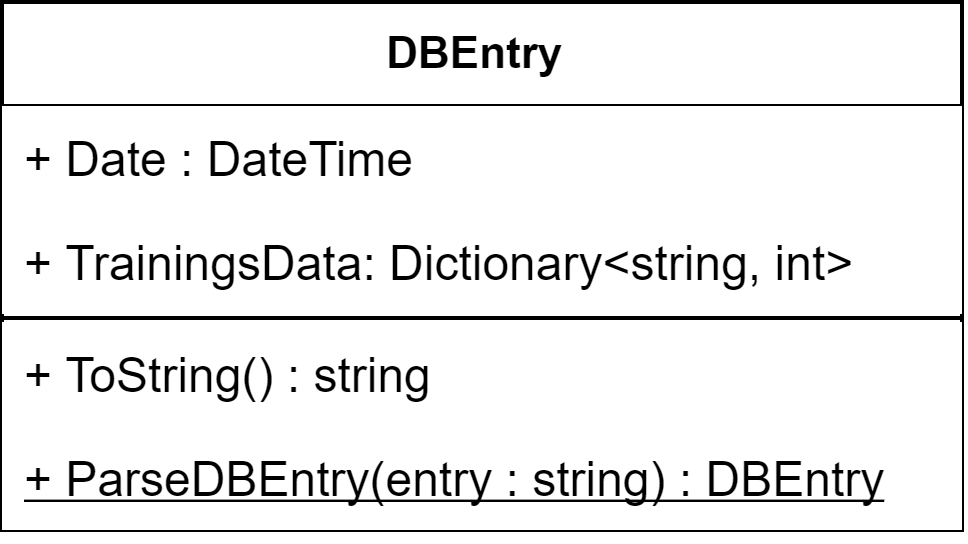
\includegraphics[width=\textwidth]{bilder/EMKlassen/DBEntryClass.png}
\end{minipage}
	\paragraph{Klassenbeschreibung}
	Die Klasse DBEntry ist ein Datencontainer, welcher einen Trainingstag darstellt. Dieser wird in der Datenbank gespeichert. DBEntry beinhaltet kein selbstständiges Verhalten. Für die Modularität sind die unterschiedlichen Attribute in einem Dictionary gespeichert.
	
	\paragraph{Attribute}
	\begin{itemize}
		\item[+] \textbf{Date: DateTime}\\Das Datum des Trainingstages. Wird als eindeutiger Bezeichner (Primary key) in der \Gls{Datenbank} benutzt.\\
			\item[+] \textbf{TrainingsData : Dictionary<String, int>}\\ Beinhaltet die einzelnen Attribute. Dabei ist der string der Bezeichner des Attributes und int die Anzahl der Inhalt. 
	\end{itemize}
	 
	 \paragraph{Methoden}
	 \begin{itemize}
	 	\item[+] \textbf{<<override>> ToString(): string}\\Liefert die Instanz als string zurück. Dabei wird das \gls{CSV}-Format verwendet. Als Attribute werden standardgemäß die Schritte (Steps), Liegestützen (PushUps) und die SitUps gespeichert.
	 	Beispiel: ``11.11.19,PushUps=10,SitUps=2,Steps=242''\\
	 	\item[+] \textbf{static ParseDBEntry(entry: string) : DBEntry}\\Liest aus einem string ein DBEntry Objekt. Falls der string nicht dem Format entspricht, wird null zurückgegeben. Das Format ist in ToString() festgelegt.\\
	\end{itemize}











\section{Klassenbeschreibung ViewModel}
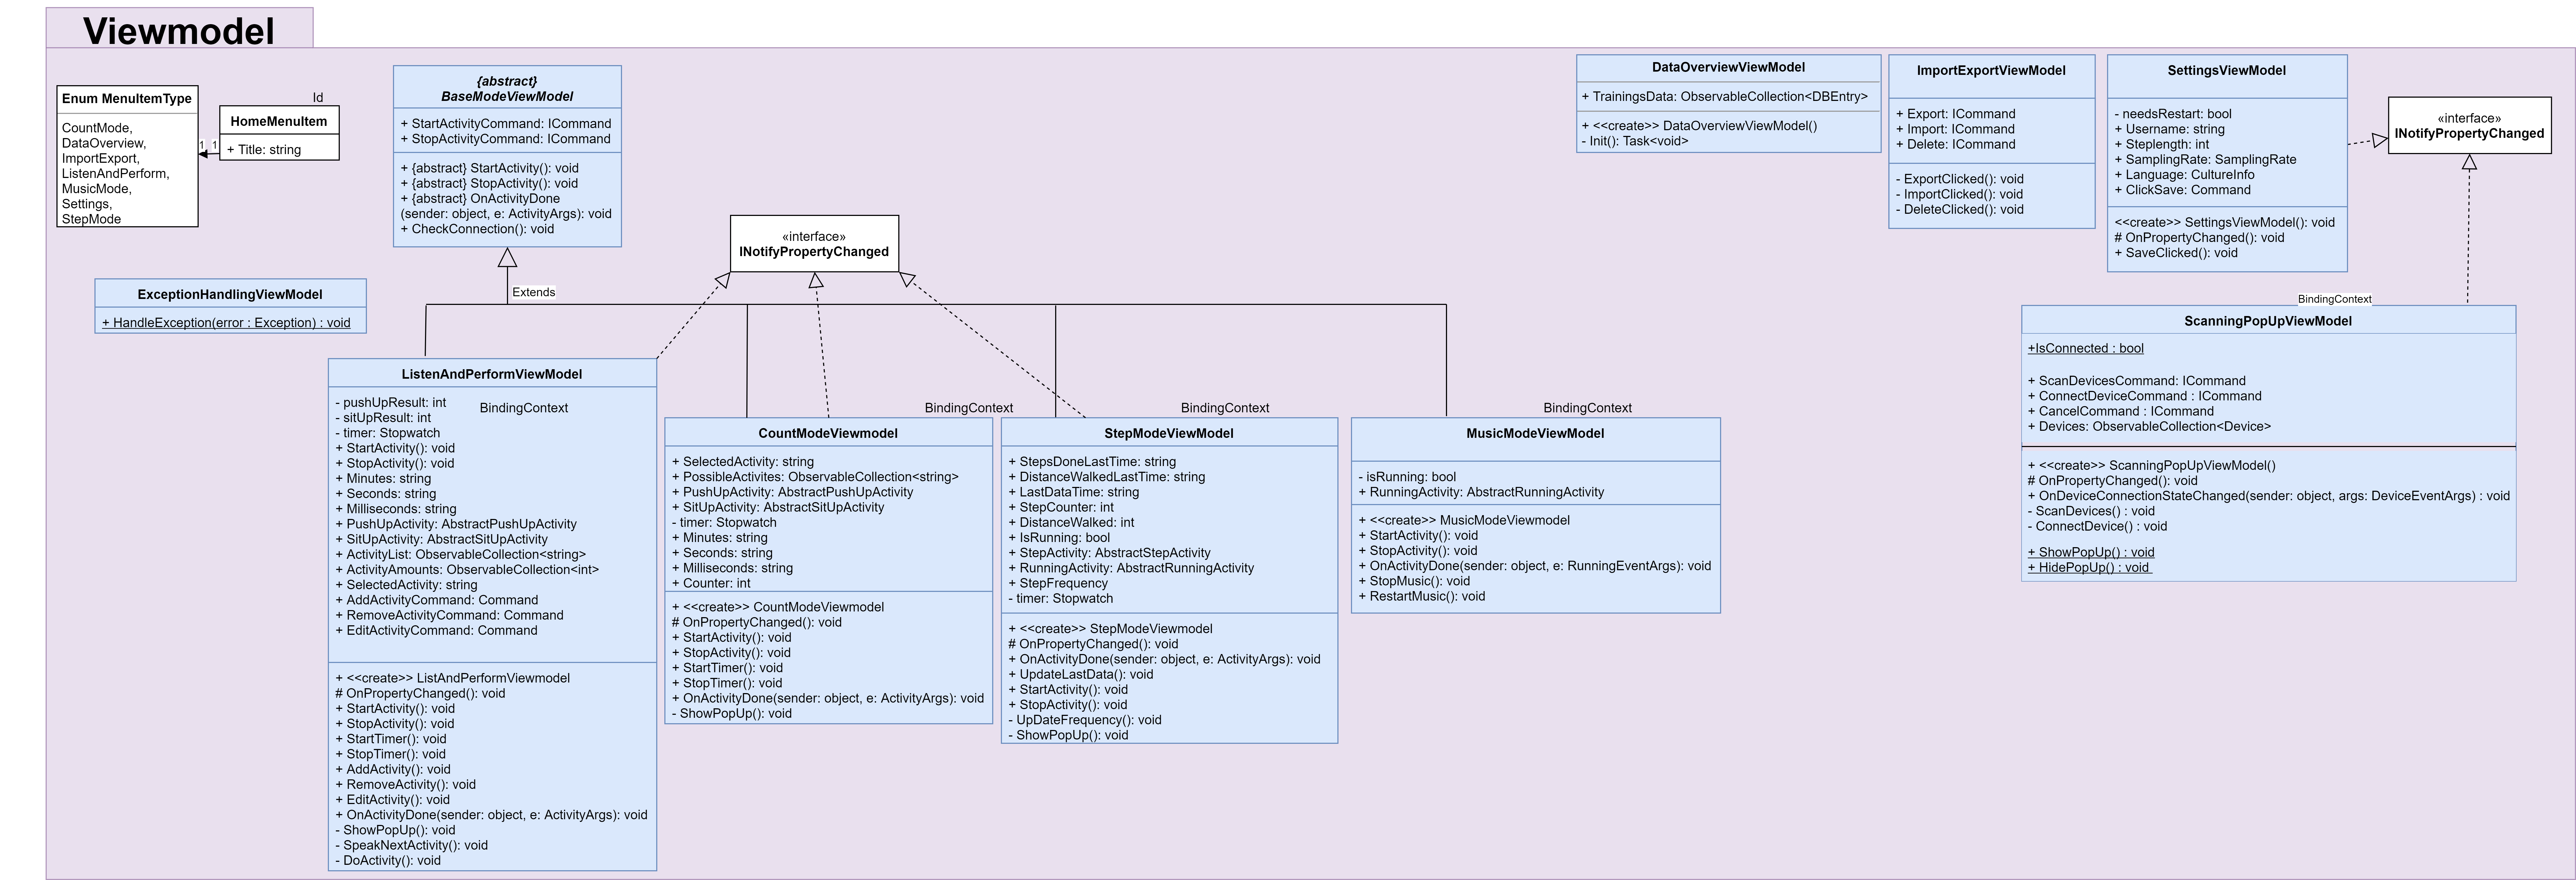
\includegraphics[width=\textwidth]{Diagramme/uebersicht/Viewmodel}
\subsection{Abstract Class BaseModeViewModel} 
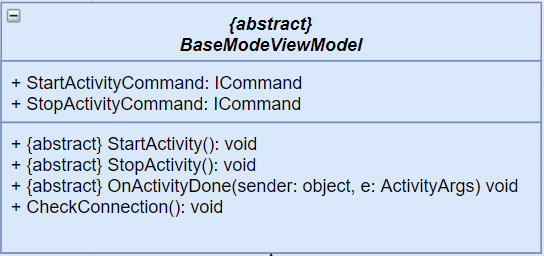
\includegraphics{bilder/ViewModelKlassen/BaseModeViewModel}

\paragraph{Klassenbeschreibung:}
Die abstrakte Klasse IBaseModeViewModel hält die Commands für Buttonklicks, die in jedem ViewModel der einzelnen Modi benötigt werden. Die Methoden die von den Commands aufgerufen werden und die Event Methode werden als abstrakt deklariert und in den Unterklassen implementiert. Die CheckConnection Methode wird beim Starten eines Vorgangs aufgerufen und ist bereits implementiert.
\paragraph{Attribute:}
\begin{itemize}
	\item[+] \textbf{StartActivityCommand: ICommand} \\  Der Command der beim Drücken des Start Buttons ausgeführt wird, um einen Vorgang zu starten. Ruft die StartActivity Methode auf.
	\item[+] \textbf{StopActivityCommand: ICommand} \\ Der Command der beim Drücken des Stop Buttons ausgeführt wird, um den Laufvorgang zu stoppen. Ruft die StoptActivity Methode auf.
\end{itemize} 
\paragraph{Methoden:}
\begin{itemize}
	\item[\#] \textbf{abstract StartActivity(): void} \\ Abstrakte Methode, die vom StartActivityCommand aufgerufen wird und in den Unterklassen spezifiziert wird.
	\item[\#] \textbf{abstract StopActivity(): void} \\ Abstrakte Methode, die vom StopActivityCommand aufgerufen wird und in den Unterklassen spezifiziert wird.
	\item[\#] \textbf{CheckConnection(): void} \\ Methode, die vom statischen PopUpViewModel den Verbindungsstatus abfragt und bei Bedarf eine Verbindung mit den \Gls{Earables} herstellt.
	\item[+] \textbf{abstract OnActivityDone(sender: object, e: ActivityArgs):void} \\ Abstrakte Methode deren Implementierung in den Unterklassen von den Eventhandlern der Activities aufgerufen wird.
	
\end{itemize}


	\subsection{Class StepModeViewModel}

	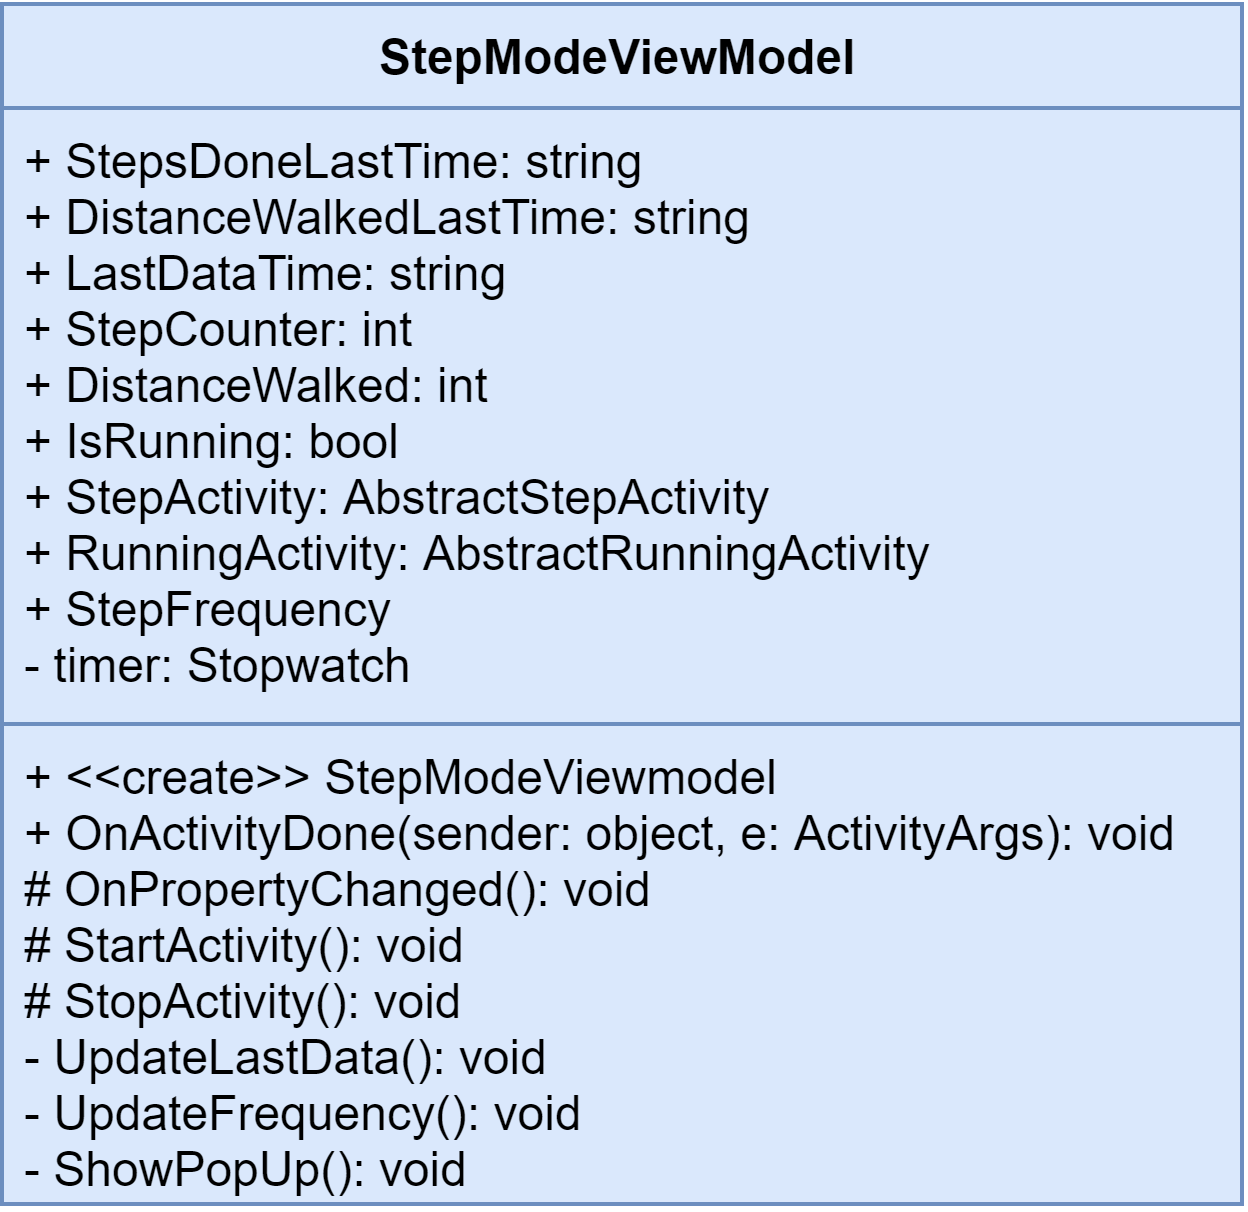
\includegraphics{bilder/ViewModelKlassen/StepModeViewModel.png}

\paragraph{Klassenbeschreibung:}
Die Klasse StepModeViewModel erbt von der abstrakten Klasse BaseModeViewModel, enthält die Logik des Stepmodes  und hält Attribute die per Databinding an die Viewklassen StepModePage und StepModeActivePage gebunden sind. 
\paragraph{Attribute:}
\begin{itemize}
	\item[$-$] \textbf{stepActivity: AbstractStepActivity} \\ Die vom ServiceManager gelieferte Singleton-StepActivity.
	\item[$-$] \textbf{runningActivity: AbstractRunningActivity} \\ Die vom ServiceManager gelieferte Singleton-RunningActivity.
	\item[$-$] \textbf{timer: Stopwatch} \\ Timer, um die Schrittfrequenz zu messen.
	\item[+] \textbf{StepsDoneLastTime: string} \\ Hält die Schrittanzahl des letzten aktiven Laufvorgangs. 
	\item[+] \textbf{DistanceWalkedLastTime: string} \\ Hält die gelaufene Distanz während des letzten aktiven Laufvorgangs. 
	\item[+] \textbf{LastDatatime: string} \\ Hält das Datum des letzten aktiven Laufvorgangs. 
	\item[+] \textbf{StepCounter: int} \\ Counter für die Schrittanzahl während des aktiven Laufvorgangs. 
	\item[+] \textbf{DistanceWalked: int} \\  Bisher gelaufene Distanz während des aktiven Laufvorgangs.
	\item[+] \textbf{IsRunning: bool} \\ True wenn der Nutzer läuft, false wenn er steht. 
	\item[+] \textbf{StepFrequency: int} \\ Aktuelle Schrittfrequenz des Nutzers.
\end{itemize}
\paragraph{Methoden:}
\begin{itemize}
	\item[+] \textbf{<<create>> StepModeViewModel()}\\ Konstruktor, in dem die Commands definiert werden. Die Anzahl der zuletzt gelaufenen Schritte und die Distanz sowie das Datum werden durch Aufruf der Methode updateLastData über den ServiceManager von der DatabaseConnection aktualisiert. isRunning wird standardmäßig zunächst auf false gesetzt. Die beiden Activity Attribute StepActivity und RunningActivity werden ebenfalls über den ServiceManager initialisiert.
	\item[+] \textbf{OnActivityDone(sender: object, e: ActivityArgs): void} \\ Event Methode, die von der Aktivität bei Erkennung von einem Schritt aufgerufen wird. Sie erhöht den Counter um 1 und setzt IsRunning auf True. 
	\item[\#] \textbf{OnPropertyChanged(): void} Methode die beim Eintritt des PropertyChanged Events aufgerufen wird. Sie übermittelt der View die Änderungen im ViewModel.
	\item[\#] \textbf{StartActivity(): void}\\ Methode die vom StartActivityCommand aufgerufen wird. Zunächst wird mit CheckConnection der Verbindungsstatus überprüft und gegebenenfalls eine Verbindung hergestellt. Das ViewModel registriert seine OnActivityDone Event Methode beim Event Handler in der StepActivity und in der RunningActivity Klasse, setzt den StepCounter zurück, startet den Timer und wechselt zum StepModeActiveView. Nach einem festgelegten Zeitabschnitt wird die Methode UpdateFrequency aufgerufen, um die Schrittfrequenz zu ermitteln
	\item[\#] \textbf {StopActivity(): void}\\ Methode die vom StopActivityCommand aufgerufen wird. Meldet die OnActivityDone Methode vom EventHandler in der StepActivity und RunningActivity Klasse ab und setzt IsRunning auf false. Zeigt ein PopUp mit der Anzahl der gelaufenen Schritte an, welches der Nutzer wegklicken kann. Danach wird zum StepModeView zurück gewechselt, die gelaufenen Schritte mit Hilfe der DatabaseConnection gespeichert und die Anzeige des letzten Laufvorgangs aktualisiert.  
	\item[$-$] \textbf{UpdateLastData(): void} \\ Wird vom Konstruktor und nach jedem Laufvorgangsende aufgerufen. Aktualisiert die Attribute StepsDoneLastTime, DistanceWalkedLastTime und LastDatatime, indem über den Service Manager von der DataBaseConnection der letzte Eintrag genommen wird. 
	\item[$-$] \textbf{UpdateFrequency(): void} \\ Berechnet nach einer festgelegten Zeit aus der abgelaufenen Zeit und der Schrittanzahl die aktuelle Schrittfrequenz.
	\item[$-$] \textbf{ShowPopUp(): void} \\ Zeigt das PopUp mit den gelaufenen Schritten und der Distanz (Vorgangsresultaten) asynchron an, wegklickbar mit einem Button.
\end{itemize}


	\subsection{Class CountModeViewModel}

	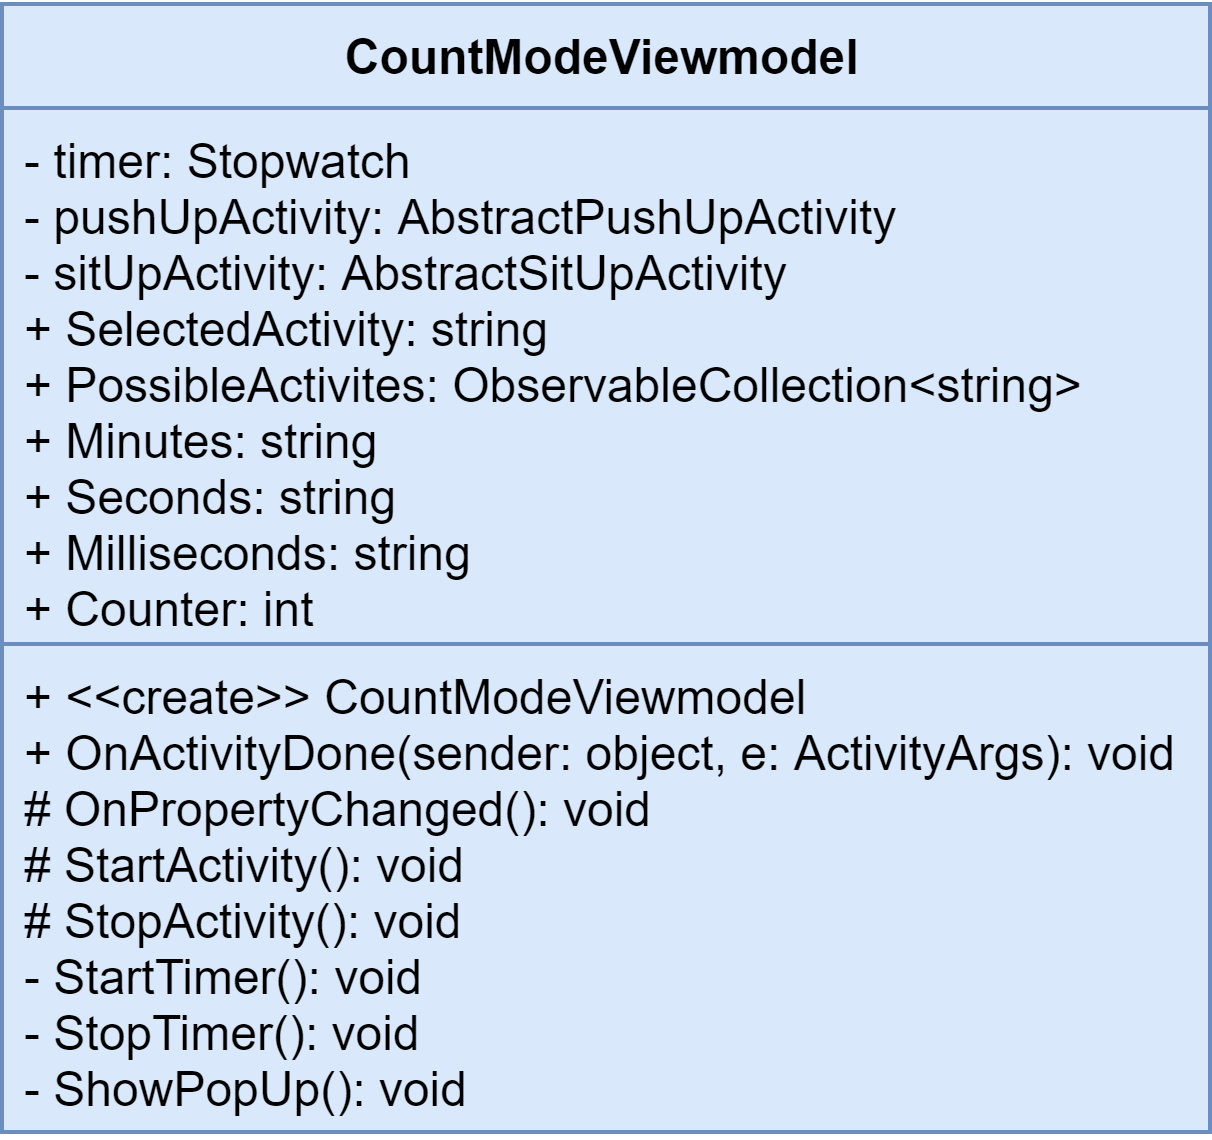
\includegraphics{bilder/ViewModelKlassen/CountModeViewModel}

\paragraph{Klassenbeschreibung:}
Die Klasse CountModeViewModel erbt von der abstrakten Klasse BaseModeViewModel, enthält die Logik des Countmodes und hält Attribute die per Databinding an die Viewklassen CountModePage und CountModeActivePage gebunden sind.
\paragraph{Attribute:}
\begin{itemize}
	\item[$-$] \textbf{pushUpActivity: AbstractPushUpActivity} \\ Die vom ServiceManager gelieferte Singleton-Activity.
	\item[$-$] \textbf{sitUpActivity: AbstractSitUpActivity} \\ Die vom ServiceManager gelieferte Singleton-Activity. 
	\item[$-$] \textbf{timer: Stopwatch} \\ Der Timer, welcher die Trainingszeit des Nutzers misst.
	\item[+] \textbf{SelectedActivity: string} \\ Die aktuell vom Nutzer im Menü ausgewählte Aktivität. 
	\item[+] \textbf{PossibleActivities: ObservableCollection<string>} \\ Die möglichen Aktivitäten die vom Nutzer ausgewählt werden können. 
	\item[+] \textbf{Minutes: string} \\ Anzahl Minuten der Ausführungszeit. 
	\item[+] \textbf{Seconds: string} \\ Anzahl Sekunden der Ausführungszeit. 
	\item[+] \textbf{Milliseconds: string} \\ Anzahl Millisekunden der Ausführungszeit. 
	\item[+] \textbf{Counter: int} \\ Ein Zähler, der die Anzahl der ausgeführten Wiederholungen des Nutzers zählt. 
\end{itemize}
\paragraph{Methoden:}
\begin{itemize}
	\item[+] \textbf{<<create>> CountModeViewModel()} \\ Konstruktor, in dem die Commands definiert werden. Die beiden Activity Attribute PushUpActivity und SitUpActivity werden über den ServiceManager initialisiert. In die PossibleActivities Liste werden SitUps und PushUps hinzugefügt.
	\item[+] \textbf{OnActivityDone(sender: object, e:ActivityArgs): void} \\ Event Methode, die von der Aktivität bei Erkennung der Ausführung von einer Wiederholung aufgerufen wird. Sie erhöht den Counter um 1. 
	\item[\#] \textbf{OnPropertyChanged(): void} Methode die beim Eintritt des PropertyChanged Events aufgerufen wird. Sie übermittelt der View die Änderungen im ViewModel.
	\item[\#] \textbf{StartActivity(): void} \\ Methode die vom StartActivityCommand aufgerufen wird. Zunächst wird mit CheckConnection der Verbindungsstatus überprüft und gegebenenfalls eine Verbindung hergestellt. Das ViewModel registriert seine OnActivityDone Event Methode beim Event Handler in der Activity Klasse und wechselt zum CountModeActivePage; danach wird der Timer gestartet. 
	\item[\#] \textbf{StopActivity(): void} \\ Methode die vom StopActivityCommand aufgerufen wird. Meldet die OnActivityDone Methode vom EventHandler in der Activity Klasse ab und hält den Timer an. Zeigt ein PopUp mit der Anzahl der ausgeführten Aktivität an, welches der Nutzer wegklicken kann. Danach werden die Anzahl der ausgeführten Wiederholungen mit Hilfe der DatabaseConnection gespeichert und zum CountModePage zurück gewechselt. 
	\item[$-$] \textbf{StartTimer(): void} \\ Startet den Timer. 
	\item[$-$] \textbf{StopTimer(): void} \\ Stoppt den Timer. 
	\item[$-$] \textbf{ShowPopUp(): void} \\ Zeigt das PopUp mit dem Vorgangsresultat asynchron an, wegklickbar mit einem Button. 
\end{itemize}



	\subsection{Class ListenAndPerformViewModel}

	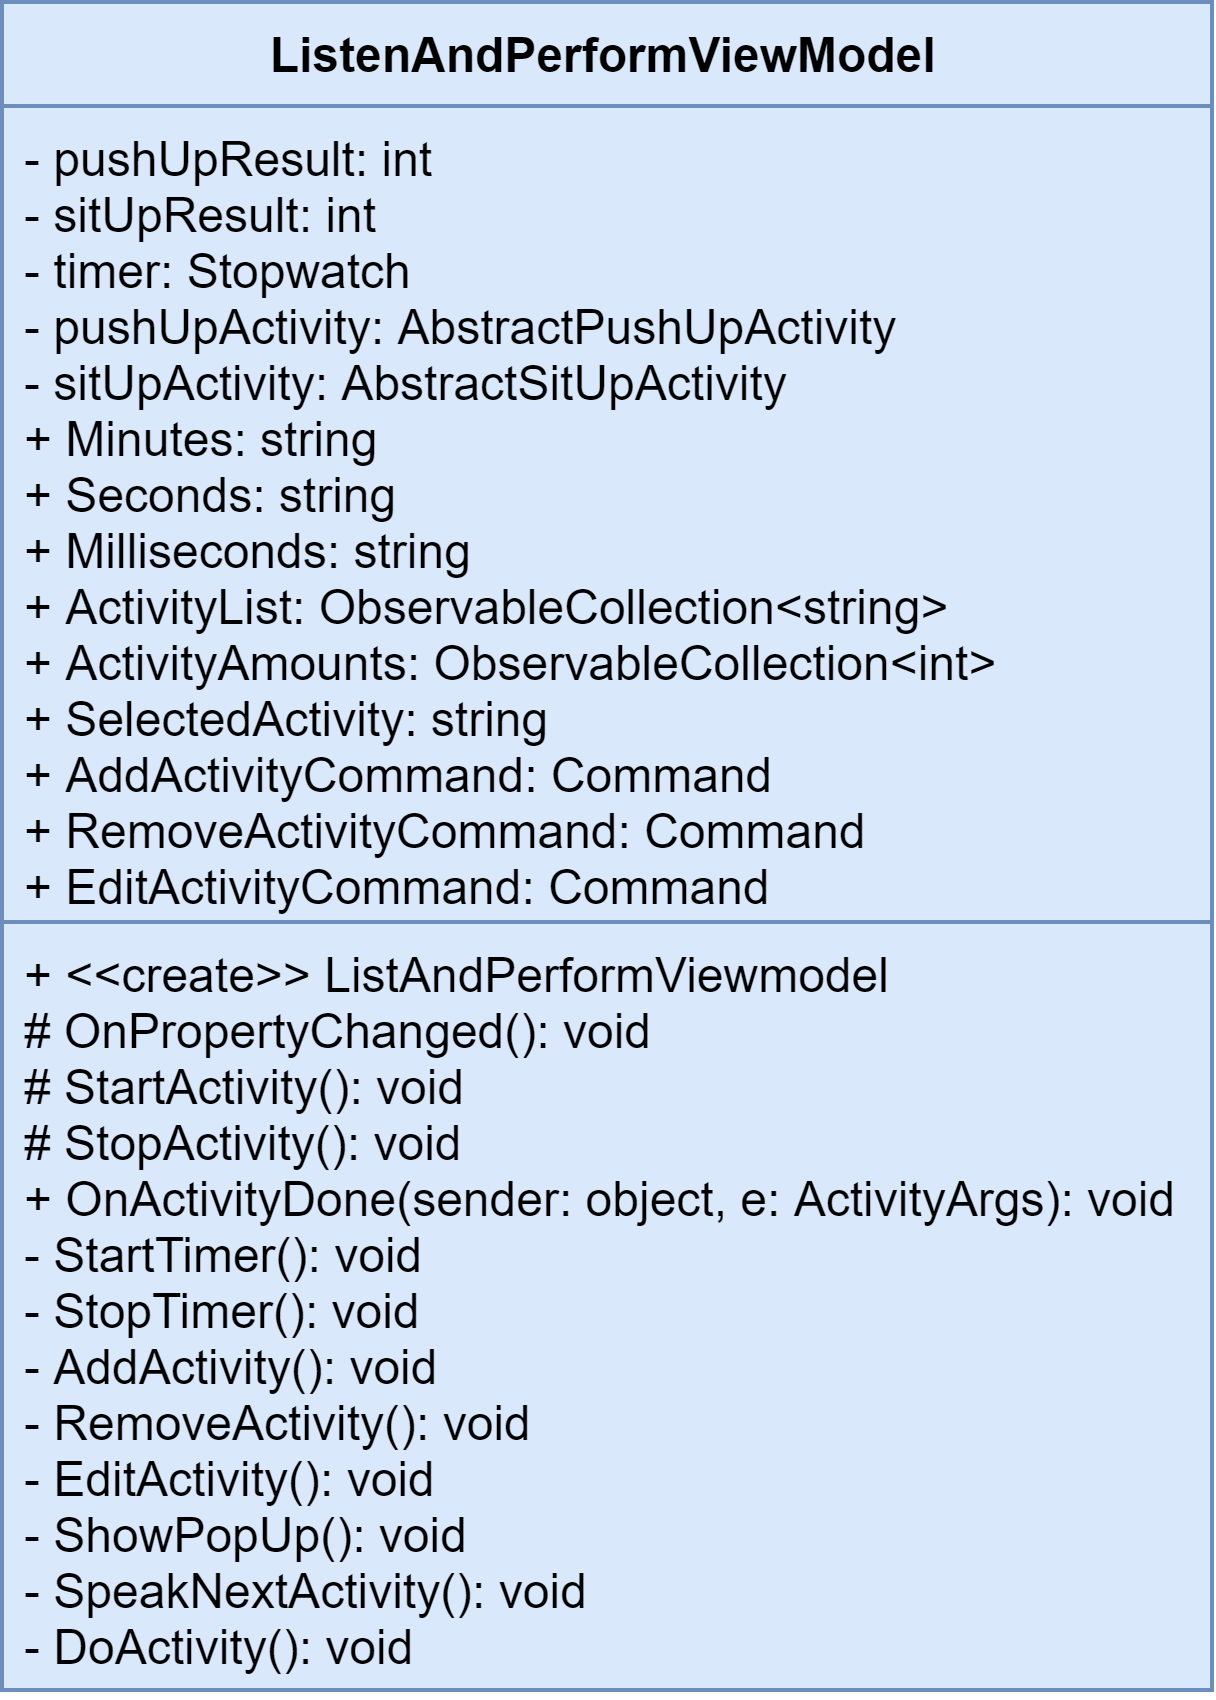
\includegraphics{bilder/ViewModelKlassen/ListenAndPerformViewModel}

\paragraph{Klassenbeschreibung:}
Die Klasse ListenAndPerformViewModel erbt von der abstrakten Klasse BaseModeViewModel, enthält die Logik von Listen\&Perform und hält Attribute die per Databinding an die Viewklassen CountModePage und CountModeActivePage gebunden sind.  Sie implementiert die INotifyPropertyChanged Schnittstelle, um das Erstellen eines Trainingsablaufplans durch den Benutzer in der zugehörigen Viewklasse anzeigen zu können.
\paragraph{Attribute:}
\begin{itemize}
	\item[$-$] \textbf{pushUpResult: int} \\ Zähler für insgesamt während des aktuellen Trainings ausgeführte Push-ups. 
	\item[$-$] \textbf{sitUpResult: int} \\ Zähler für insgesamt während des aktuellen Trainings ausgeführte Sit-ups. 
	\item[$-$] \textbf{timer: Stopwatch} \\ Der Timer, welcher die Trainingsdauer des Nutzers misst. 
	\item[$-$] \textbf{pushUpActivity: AbstractPushUpActivity} \\ Die vom ServiceManager gelieferte Singleton-Activity.
	\item[$-$] \textbf{sitUpActivity: AbstractSitUpActivity} \\ Die vom ServiceManager gelieferte Singleton-Activity.
	\item[+] \textbf{Minutes: string} \\ Anzahl Minuten der Trainingszeit. 
	\item[+] \textbf{Seconds: string} \\  Anzahl Sekunden der Trainingszeit. 
	\item[+] \textbf{Milliseconds: string} \\ Anzahl Sekunden der Trainingszeit. 
	\item[+] \textbf{ActivityList: ObservableCollection<string>} \\ Liste der Aktivitäten die der Nutzer durchführen möchte, die durch ihn anpassbar ist. 
	\item[+] \textbf{ActivityAmounts: ObservableCollection<int>} \\ Anzahl der Aktivitäten die der Nutzer durchführen möchte; durch ihn anpassbar. 
	\item[+] \textbf{SelectedActivity: string} \\ Hilfsattribut zum Bearbeiten und Löschen eines Listeneintrags. Per Databinding an die View gebunden; es ist der Eintrag der Liste auf den der Nutzer zuletzt getippt hat. 
	\item[+] \textbf{AddActivityCommand: Command} \\ Der Command der beim Drücken des AddActivity Buttons ausgeführt wird. 
	\item[+] \textbf{RemoveActivityCommand: Command} \\ Der Command der beim Drücken des RemoveActivity Buttons ausgeführt wird. 
	\item[+] \textbf{EditActivityCommand: Command} \\ Der Command der beim Drücken des EditActivity Buttons ausgeführt wird. 
\end{itemize}
\paragraph{Methoden:}
\begin{itemize}
	\item[+] \textbf{<<create>> ListAndPerformViewModel} \\ Konstruktor, in dem die Commands definiert werden. Die ActivityList und ActivityAmounts werden initialisiert. Die beiden Activity Attribute PushUpActivity und SitUpActivity werden über den ServiceManager initialisiert.
	\item[\#] \textbf{OnPropertyChanged(): void} \\ Methode die beim Eintritt des PropertyChanged Events aufgerufen wird. Sie verändert bei der registrierten View Klasse die Anzeige der ausgewählten Aktivitäten sowie deren Anzahl. 
	\item[\#] \textbf{StartActivity(): void} \\ Methode die vom StartActivityCommand aufgerufen wird. Zunächst wird mit CheckConnection der Verbindungsstatus überprüft und gegebenenfalls eine Verbindung hergestellt. Die Methode wechselt dann zur ListenAndPerformActivePage. Ruft für jeden Listeneintrag in ActivityList nacheinander die DoActivity Methode auf, bis die Liste abgearbeitet ist. Nach Abarbeiten der Liste wird automatisch die Methode StopActivity aufgerufen.
	\item[\#] \textbf{StopActivity(): void} \\ Methode die vom StopActivityCommand aufgerufen wird. Hält den Timer an und zeigt ein PopUp mit der Anzahl der ausgeführten Aktivitäten an, welches der Nutzer wegklicken kann. Danach werden die Anzahl der ausgeführten Wiederholungen mit Hilfe der DatabaseConnection gespeichert und zur ListenAndPerformPage zurück gewechselt. 
	\item[+] \textbf{ OnActivityDone(sender: object, e: ActivityArgs): void} \\ Event Methode, die von der Aktivität bei Erkennung der Ausführung von einer Wiederholung aufgerufen wird. Sie erhöht den jeweiligen Counter um 1.  
	\item[$-$] \textbf{StartTimer(): void} \\ Startet den Timer. 
	\item[$-$] \textbf{StopTimer(): void} \\ Stoppt den Timer. 
	\item[$-$] \textbf{ AddActivity(): void} \\  Methode die vom AddActivityCommand aufgerufen wird. Ein Popup erscheint, bei dem der Nutzer auf Liegestütze, Situp oder Pause drücken kann. Nach dem Bestätigen wird erscheint ein neues Popup mit der Anzahl. Die Auswahl wird zu den jeweiligen Listen hinzugefügt. 
	\item[$-$] \textbf{RemoveActivity(): void} \\  Methode die vom RemoveActivityCommand aufgerufen wird. Der gehaltene SelectedActivity Eintrag wird entfernt. 
	\item[$-$] \textbf{EditActivity(): void} \\ Methode die vom EditActivityCommand aufgerufen wird. Der gehaltene SelectedActivity Eintrag wird vom Nutzer editiert.
	\item[$-$] \textbf{ShowPopUp(): void} \\ Zeigt das PopUp mit dem Vorgangsresultat asynchron an, wegklickbar mit einem Button. 
	\item[$-$] \textbf{SpeakNextActivity(): void} \\ Liest die nächste Aktivität der ActivityList sowie seine Anzahl asynchron vor. 
	\item[$-$] \textbf{DoActivity(): void} \\ Das ViewModel registriert seine seine OnActivityDone Event Methode bei der aktuellen Activity der ActivityList. Liest die Activity vor und startet den Timer. Nach Erkennung der vorher festgelegten Anzahl Wiederholungen, meldet das ViewModel seine OnActivityDone Methode ab und zählt den entsprechenden ResultCounter um die ausgeführte Anzahl hoch. \\
\end{itemize}


	\subsection{Class MusicModeViewModel}
	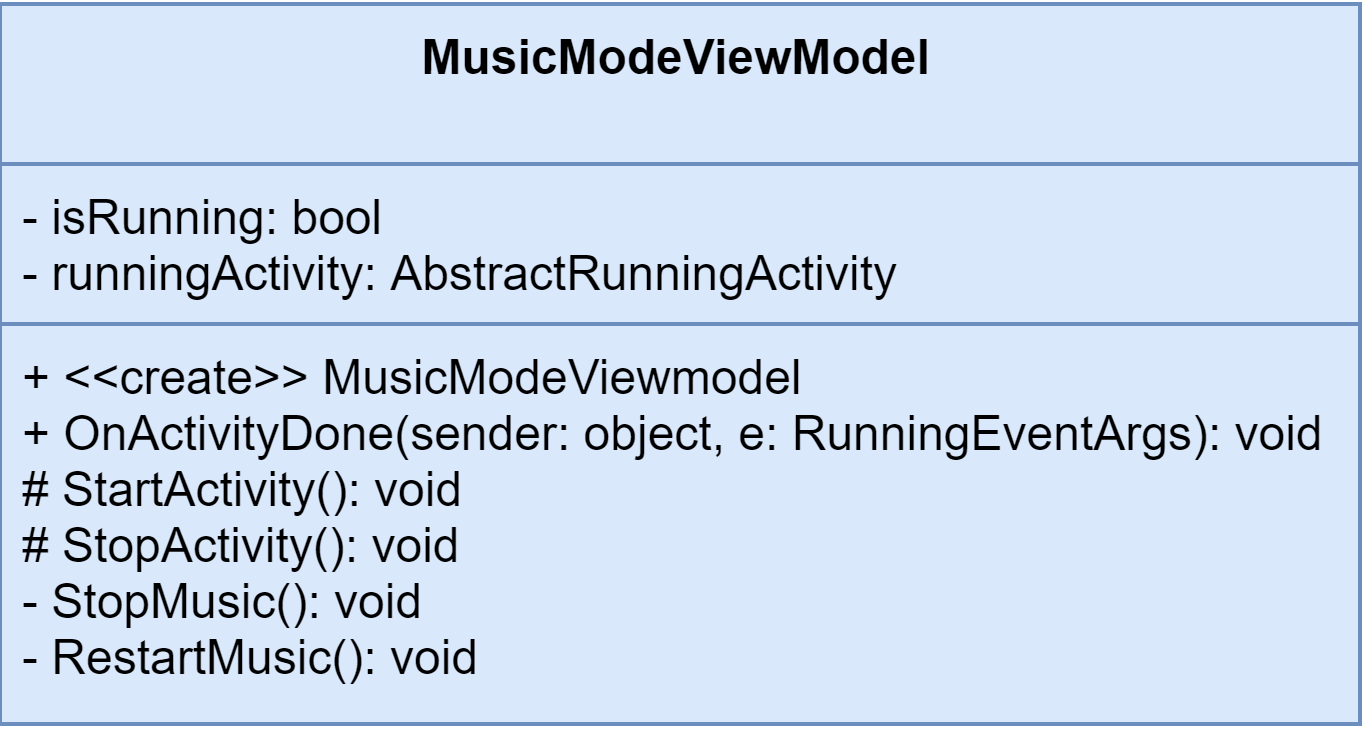
\includegraphics{bilder/ViewModelKlassen/MusicModeViewModel}
\paragraph{Klassenbeschreibung:}
Die Klasse MusicModeViewModel erbt von der abstrakten Klasse BaseModeViewModel und enthält die Logik des Musicmodes.
\paragraph{Attribute:}
\begin{itemize}
	\item[$-$] \textbf{isRunning: boolean} \\ Hilfsattribut, speichert ob der Nutzer steht oder läuft, wird in der View nicht angezeigt.
	\item[$-$] \textbf{runningActivity: AbstractRunningActivity} \\ Die vom ServiceManager gelieferte Singleton-RunningActivity.
\end{itemize}
\paragraph{Methoden:}
\begin{itemize}
	\item[+] \textbf{<<create>> MusicModeViewModel} \\ Konstruktor, in dem die Commands definiert werden. Das Activity Attribut RunningActivity wird über den ServiceManager initialisiert.
	\item[+] \textbf{OnActivityDone(sender: object, e: RunningEventArgs): void} \\ Event Methode, die von der Activity aufgerufen wird, die gegebenenfalls isRunning ändert und die Musikmethoden aufruft.
	\item[\#] \textbf{StartActivity(): void} \\ Methode die vom StartActivityCommand aufgerufen wird. Zunächst wird mit CheckConnection der Verbindungsstatus überprüft und gegebenenfalls eine Verbindung hergestellt. Registriert die OnActivityDone Methode beim EventHandler der RunningActivity. 
	\item[\#] \textbf{StopActivity(): void} \\ Methode die vom StopActivityCommand aufgerufen wird. Meldet die OnActivityDone Methode beim EventHandler der RunningActivity ab. 
	\item[$-$] \textbf{StopMusic(): void} \\ Wird von OnActivityDone aufgerufen wenn der Nutzer stehen bleibt. Hält die Musik an.
	\item[$-$] \textbf{RestartMusic(): void} \\ Wird von OnActivityDone aufgerufen wenn der Nutzer weiter läuft. Spielt die Musik weiter ab.
\end{itemize}

	\subsection{Class DataOverviewViewModel}

	\includegraphics[width=0.5\linewidth]{bilder/ViewModelKlassen/DataOverviewViewModel.png}

\paragraph{Klassenbeschreibung:}
Das DataOverviewViewModel läd die Trainingsdaten des Nutzers über den Datenbank Service und bindet diese an die ListView \textit{contentListView} der DataOverviewPage.
Mithilfe der ObservableCollection werden alle Änderungen der Liste automatisch in der DataOverviewPage angezeigt.
\paragraph{Attribute:}
\begin{itemize}
	\item[+] \textbf{TrainingsData: ObservableCollection<DBEntry>}
\end{itemize}
Die Commands werden je an den entsprechenden Button im View gekoppelt und lösen die entsprechende Methode in dieser Klasse aus.
\paragraph{Methoden:}
\begin{itemize}
    \item[+] \textbf{<<create>> DataOverviewViewModel()} \\ Setzt die \textit{ItemsSource} der contentListView auf \textit{TrainingsData} und ruft \textit{Init()} auf.
    \item[$-$] \textbf{Init(): void} \\ Kapselt den asynchronen Aufruf zu \textit{GetMostRecentEntriesAsync} des \textit{IDataBaseConnection} Service.
\end{itemize} 

\begin{minipage}[t]{0.8\textwidth}

	\subsection{Class ImportExportViewModel}

\end{minipage}
\begin{minipage}[c]{0.2\textwidth}
	\includegraphics[width=\textwidth]{bilder/ViewModelKlassen/ImportExportViewModel}
\end{minipage}
\paragraph{Klassenbeschreibung:}
Das ImportExportViewModel verarbeitet das Klicken des Nutzers auf die Buttons  der ImportExportPage.
Die Kommunikation wird dabei mit Commands geregelt.
\paragraph{Attribute:}
\begin{itemize}
	\item[+] \textbf{Export: ICommand}\\Der Command, welches aufgerufen wird beim Klicken auf den Button 'Export'. Ruft die Methode ExportClicked auf.
	\item[+] \textbf{Import: ICommand}\\Der Command, welches aufgerufen wird beim Klicken auf den Button 'Import'. Ruft die Methode ImportClicked auf.
	\item[+] \textbf{Delete: ICommand}\\Der Command, welches aufgerufen wird beim Klicken auf den Button 'Delete'. Ruft die Methode DeleteClicked auf.
\end{itemize}
Die Commands werden an die entsprechenden Buttons im View gekoppelt und lösen die entsprechende Methode in dieser Klasse aus.
\paragraph{Methoden:}
\begin{itemize}
    \item[$-$] \textbf{exportClicked(): void}\\ Öffnet einen folderPicker-Dialog und ruft danach in IDataBaseConnection exportTrainingData mit dem vom Nutzer im Dialog ausgewählten Pfad aus.%%??name genau von dem filePicker??
    \item[$-$] \textbf{importClicked(): void}\\ Öffnet einen filePicker-Dialog und ruft danach in IDataBaseConnection importTrainingData mit dem vom Nutzer ausgewählten file auf.
    \item[$-$] \textbf{deleteClicked(): void}\\Zeigt einen Warning-Dialog an, ob man wirklich alle Vorgangsdaten löschen will. Daraufhin wird bei Bestätigung in IDatabaseConnection deleteTrainingData aufgerufen.
\end{itemize} 

	\subsection{Class SettingsViewModel}

	\includegraphics{bilder/ViewModelKlassen/SettingsViewModel.png}
\paragraph{Klassenbeschreibung:}
Die Klasse SettingsViewModel enthält die Logik der SettingsPage. Sie erbt von INotifyPropertyChanged und verwendet für das Speichern der Einstellungen einen Command. Außerdem holt sie sich vom SettingsService alle aktuellen Einstellungen.
\paragraph{Attribute:}
\begin{itemize}
	\item[$-$] \textbf{needsRestart: bool}\\ Diese Property verfügt nur über einen privaten Getter. Sie ist genau dann wahr, wenn der Nutzer die Sprache geändert hat, also der Zustand des Sliders in der View und der Zustand als in dieser Klasse als Attribut gespeicherten Sprache unterschiedlich sind.

	\item[+] \textbf{Username: string}\\Der Username verfügt über ein Binding zur View.
	\item[+] \textbf{StepLength: int}\\Die StepLength verfügt über ein Binding zur View. 
	\item[+] \textbf{SamplingRate: SamplingRate}\\Die aktuell eingestellte Samplerate. Dieses Attribut wird nicht direkt im View gebunden.
	\item[+] \textbf{Language: CultureInfo}\\Die aktuell eingestellte Sprache. Dieses Attribut wird nicht direkt im View gebunden. 
	\item[+] \textbf{ClickSave: Command}\\Bei Ausführen dieses Commands wird die Methode SaveClicked ausgeführt. 
\end{itemize}
\paragraph{Methoden:}
\begin{itemize}
    \item[+] \textbf{<<create>> SettingsViewModel(): void}\\ Im Konstruktor holt sich die Klasse vom ISettingsService den User, die Sprache und die Samplingrate und speichert die Entsprechenden Werte in den eigenen Properties. Die Werte von Attributen, die über kein Binding verfügen, müssen hier manuell ins View übertragen werden.
    \item[\#] \textbf{OnPropertyChanged(): void}\\ Die Methode wird von der Schnittstelle INotifyPropertyChanged geerbt. Diese wird benutzt um die View zu aktualisieren und ihr um Bescheid zu geben, wenn sich eine Eigenschaft aus dem ViewModel verändert. 
    \item[$-$] \textbf{SaveClicked(): void}\\ wenn diese Methode aufgerufen wird, werden die aktuellen Properties wieder im ISettingsService gespeichert, nachdem alle Werte von Attributen, die über kein Binding verfügen, vom View geholt und aktualisiert werden. Bei Auftretenden Exceptions (kein Gerät verbunden) wird eine Fehlermeldung als Popup angezeigt. Liefert needsRestart wahr, wird außerdem ein Hinweis angezeigt, dass die App neu gestartet werden muss, um alle Änderungen zu übernehmen.\\

\end{itemize} 


\subsection{Class ScanningPopUpViewModel}
	\includegraphics{bilder/ViewModelKlassen/ScanningPopUpViewModelClass.png}
	\paragraph{Klassenbeschreibung:}
	Die Klasse ScanningPopUpViewModel ist das ViewModel zu dem View PopUpScanningPage und verwaltet die Logik dieser Komponente mithilfe von verknüpften Commands. Dabei implementiert die Klasse die Schnittstelle INotifyPropertyChanged, um die View zu aktualisieren.
	Sie benutzt die Erweiterung \Gls{Rg.Plugins.Popup} für das Anzeigen und das Versteckend des Pop-ups.
	
	\paragraph{Attribute:}
	\begin{itemize}
		\item[+] \textbf{static IsConnected: bool}\\Statisches Attribut, ob das Gerät mit den \gls{Earables} verbunden ist.
		\item[+] \textbf{ScanDevicesCommand: ICommand}\\Command, welches die Implementierung des Scannen abkapselt. Dieses Command wird ausgeführt, wenn der ScanDevice Button im View betätigt wird. Es wird die private Methode ScanDevices() aufgerufen.
		\item[+] \textbf{ConnectDeviceCommand: ICommand}\\Command, welches die Implementierung des Verbinden mit einem ausgewählten BLE Gerät aus dem ListView des Pop-ups. Es wird die private Methode ConnectDevice() aufgerufen.
		\item[+] \textbf{CancelCommand: ICommand}\\Command, welches die Implementierung des Abbrechen abkapselt. Dieses Command wird ausgeführt, wenn der Cancel Button im View betätigt wird. Es wird die public und statische Methode HidePopUp() aufgerufen. 
		\item[+] \textbf{Devices: ObservableCollection<Device>}\\Die Liste Devices dient zur Aktualisierung des Views PopUpScanningPage. Die ListView im View setzt Devices als Ressource. Da Devices eine ObservableCollection ist, wird die Listview bei einer Änderung der Deviceliste aktualisiert.
	\end{itemize}

	\paragraph{Methoden:}
	\begin{itemize}
		\item[+] \textbf{<<create>> ScanningPopUpViewModel()}\\Der Konstruktor für die Klasse ScanningPopUpViewModel. In dieser Methode, werden die Commands initialisiert. Zudem wird sich bei dem EventHandler DeviceConnectionStateChanged in der Klasse EarablesConnection im Model mit der Methode OnDeviceConnectionStateChanged(...) registriert.
		\item[\#] \textbf{OnPropertyChanged(): void}\\Die Methode wird von der Schnittstelle INotifyPropertyChanged geerbt. Diese wird benutzt um die View zu aktualisieren und ihr um Bescheid zu geben, wenn sich eine Eigenschaft aus dem ViewModel verändert.
		\item[+] \textbf{OnDeviceConnectionStateChanged(sender: object, args: DeviceEventArgs): void}\\Mit dieser Methode registrierst das ViewModel bei dem EventHandler DeviceConnectionStateChanged. In dieser wird das statische Attribut IsConnected angepasst. Falls sich das Device disconnected hat, wird die Methode ShowPopUp() aufgerufen.
		\item[$-$] \textbf{ScanDevices(): void}\\Private Methode, welche im Command ConnectDeviceCommand benutzt wird. In dieser wird die EarableConnection nach erreichbaren Geräten gefragt. Dafür wird die Methode StartScanning() aufgerufen. Die zurückgelieferte Liste an Devices wird in dem Pop-up angezeigt. Dafür wird die ListView aktualisiert. Zudem wird das erste Device in der ListView ausgewählt.
		\item[$-$] \textbf{ConnectDevice(): void}\\Private Methode, welche im Command ConnectDeviceCommand aufgerufen wird. Dabei benutzt sie die Methode ConnectToDevice(device: IDevice) der Klasse EarableConnection im Model. Es wird das Device übergeben, welches in der ListView ausgewählt wurde.
		\item[+] \textbf{static ShowPopUp(): void}\\Statische Methode, welche die View PopUpScanningPage anzeigt. Diese benutzt die Erweiterung \Gls{Rg.Plugins.Popup}. Das Anzeigen geschieht mit der Methode Popupnavigation.Instance.PushAsync(new PopUpScanningPage()). Dabei wird ein neue Instanz der PopUpScanningPage erstellt. Die Methode ist statisch, da die anderen ViewModels bei einem Vorgangstart anzeigen können muss, falls noch keine Verbindung zu den \gls{Earables} besteht.
		\item[+] \textbf{static HidePopUp(): void}\\Statische Methode, welche dieView PopUpScanningPage verstecken lässt. Diese Methode benutzt die Erweiterung \Gls{Rg.Plugins.Popup}. Das Verstecken der View geschieht mit der Methode Popupnavigation.Instance.popAsync(). 
	\end{itemize}
\newpage
\begin{minipage}[b]{0.7\textwidth}

	\subsection{Class HomeMenuItem}
\end{minipage}
\begin{minipage}[c]{0.3\textwidth}
	\includegraphics[width=\textwidth]{bilder/ViewModelKlassen/HomeMenuItem.png}
\end{minipage}
	\paragraph{Klassenbeschreibung:}
	Diese Klasse spezifiziert einen Eintrag des Menüs (siehe MenuPage). 
	\paragraph{Attribute:}
	\begin{itemize}
		\item [+] \textbf{Id: MenuItemType}\\ Der Typ des Menüeintrags (in UML als Assoziation dargestellt).
		\item [+] \textbf{Title: string}\\ Der angezeigte Text des Menüeintrags.
	\end{itemize}
\begin{minipage}[b]{0.7\textwidth}

	\subsection{Enumeration MenuItemType}
\end{minipage}
\begin{minipage}[c]{0.3\textwidth}
	\includegraphics[width=\textwidth]{bilder/ViewModelKlassen/MenuItemType.png}
	\vspace{0.3cm}
\end{minipage}

	Dieses Enum spezifiziert alle möglichen Typen von Menüeinträgen der MenuPage. Entsprechend gibt es für jede vom Menü aus direkt navigierbare Page einen Wert dieses Enums. Wir orientieren uns hierbei an dem starndardmäßigen Entwurf für das Master-Detail Schema in der Entwicklungsumgebung Visual Studio 2019. \\
	\paragraph{Werte:}
	\begin{itemize}
        \item CountMode,
        \item DataOverview,
        \item ImportExport,
        \item ListenAndPerform,
        \item MusicMode,
        \item Settings,
        \item StepMode
	\end{itemize}


	\newpage
	\subsection{Class ExceptionHandlingViewModel}

	\includegraphics{bilder/ViewModelKlassen/ExceptionHandlingViewModelClass.png}

	\paragraph{Klassenbeschreibung:}
	Die Klasse ExceptionHandlingViewModel ist die zentrale Fehlerverarbeitung. Wenn eine Exception in anderen Komponenten des ViewModels oder des Models auftritt, wird die Exception gefangen und an die Klasse ExceptionHandlingViewModel weitergeleitet. Diese erstellt nun eine Benachrichtigung in Form eines DisplayAlerts, sodass der Nutzer von dieser Exception erfährt. 
	
	\paragraph{Methoden:}
	\begin{itemize}
		\item[+] \textbf{static HandleException(error: Exception): void}\\Die statische Methode HandleException nimmt als Parameter eine Instanz der Klasse Exception. In dieser Methode wird ein DisplayAlert mit dem Titel der Exception und dessen Inhalt erstellt. Der DisplayAlert wird mithilfe der MainPage angezeigt.
	\end{itemize}
\newpage
\section{Klassenbeschreibung View}
\includegraphics[width=\textwidth]{Diagramme/uebersicht/View}
\newline

\begin{minipage}[b]{0.7\textwidth}
	\subsection{Class StepModePage}
\end{minipage}
\begin{minipage}[c]{0.3\textwidth}
	\includegraphics[width=\textwidth]{bilder/ViewKlassen/StepModePage.png}
\end{minipage}
\paragraph{Klassenbeschreibung:}
Diese Klasse stellt die Ansicht des StepModes dar, solange kein Laufvorgang gestartet ist.
\paragraph{Attribute:}
	\begin{itemize}
	\item[+] \textbf{StepMode: Label} \\ Anzeige des Modusnamen Stepmode.
	\item[+] \textbf{LastTrainingsDate: Label} \\ Anzeige für den letzten Trainingstag, an das Attribut LastDataTime aus dem ViewModel gebunden.
	\item[+] \textbf{StepsDoneLastTime: Label} \\ Anzeige für die am letzten Trainingstag gelaufenen Schritte, an das Attribut StepsDoneLastTime aus dem ViewModel gebunden.
	\item[+] \textbf{DistanceWalkedLastTime: Label} \\ Anzeige für die am letzten Trainingstag gelaufene Distanz, an das Attribut DistanceWalkedLastTime aus dem ViewModel gebunden. 
	\item[+] \textbf{Start: Button} \\ Button um den Laufvorgang zu starten. Feuert den StartActivityCommand aus dem ViewModel.
	\end{itemize}

\begin{minipage}[b]{0.7\textwidth}
	\subsection{Class StepActiveModePage}
\end{minipage}
\begin{minipage}[c]{0.3\textwidth}
	\includegraphics[width=\textwidth]{bilder/ViewKlassen/StepModeActivePage.png}
\end{minipage}
\paragraph{Klassenbeschreibung:}
Diese Klasse stellt die Ansicht des Stepmodes während eines laufenden Laufvorgangs an.
\paragraph{Attribute:}
	\begin{itemize}
	\item[+] \textbf{StepMode: Label} \\ Anzeige des Modusnamen Stepmode.
	\item[+] \textbf{IsRunning: Label} \\ Zeigt an ob der Nutzer aktuell läuft oder steht, an das Attribut IsRunning aus dem ViewModel gebunden.
	\item[+] \textbf{StepCounter: Label} \\ Anzeige für Anzahl bisher gelaufener Schritte, an das Attribut StepCounter aus dem ViewModel gebunden.
	\item[+] \textbf{DistanceWalked: Label} \\ Anzeige der bisher gelaufenen Distanz, an das Attribut DistanceWalked aus dem ViewModel gebunden.
	\item[+] \textbf{StepFrequency: Label} \\ Anzeige der aktuellen Schrittfrequenz, an das Attribut StepFrequency aus dem ViewModel gebunden.
	\item[+] \textbf{Stop: Button} \\ Button um den Laufvorgang zu stoppen. Feuert den StopActivityCommand aus dem ViewModel.
	\end{itemize}
	
\begin{minipage}[b]{0.7\textwidth}
	\subsection{Class CountModePage}
\end{minipage}
\begin{minipage}[c]{0.3\textwidth}
	\includegraphics[width=\textwidth]{bilder/ViewKlassen/CountModePage.png}
\end{minipage}
\paragraph{Klassenbeschreibung:}
Diese Klasse stellt die Ansicht des Countmodes dar, solange kein Zählvorgang gestartet ist.
\paragraph{Attribute:}
	\begin{itemize}
	\item[+] \textbf{CountMode: Label} \\ Anzeige des Modusnamen CountMode.
	\item[+] \textbf{Activities: ListView} \\ Anzeige der verfügbaren Activities die auswählbar sind mithilfe einer ListView, an die ObservableCollection PossibleActivities aus dem ViewModel gebunden.
	\item[+] \textbf{Start: Button} \\ Button um den Zählvorgang zu starten. Feuert den StartActivityCommand aus dem ViewModel.
	\end{itemize}

\begin{minipage}[b]{0.7\textwidth}
	\subsection{Class CountModeActivePage}
\end{minipage}
\begin{minipage}[c]{0.3\textwidth}
	\includegraphics[width=\textwidth]{bilder/ViewKlassen/CountModeActivePage.png}
\end{minipage}
\paragraph{Klassenbeschreibung:}
Diese Klasse stellt die Ansicht des Countmodes während eines laufenden Zählvorgangs an.
\paragraph{Attribute:}
	\begin{itemize}
	\item[+] \textbf{CountMode: Label} \\ Anzeige des Modusnamen CountMode.
	\item[+] \textbf{Timer: Label} \\ Anzeige für die seit dem Zählstart vergangene Zeit. Beinhaltet drei Spans für die Anzeige von Minuten, Sekunden und Millisekunden. Das Spans sind an die Attribute Minuten, Sekunden bzw. Millisekunden gebunden.
	\item[+] \textbf{Counter: Label} \\ Anzeige für die Anzahl bisher ausgeführter Wiederholungen einer Activity. An das Attribut Counter aus dem ViewModel gebunden.
	\item[+] \textbf{SelectedActivity: Label} \\ Anzeige für die ausgewählte Übung. An das Attribut SelectedActivity aus dem ViewModel gebunden.
	\item[+] \textbf{Stop: Button} \\ Button um den Zählvorgang zu stoppen. Feuert den StopActivityCommand aus dem ViewModel.
	\end{itemize}

\begin{minipage}[b]{0.7\textwidth}
	\subsection{Class ListenAndPerformPage}
\end{minipage}
\begin{minipage}[c]{0.3\textwidth}
	\includegraphics[width=\textwidth]{bilder/ViewKlassen/ListenAndPerformPage.png}
\end{minipage}
\paragraph{Klassenbeschreibung:}
Diese Klasse stellt die Ansicht von ListenAndPerform dar, solange kein Trainingsvorgang gestartet ist.
\paragraph{Attribute:}
	\begin{itemize}
	\item[+] \textbf{ListenAndPerform: Label} \\ Anzeige des Modusnamen ListenAndPerform.
	\item[+] \textbf{WorkoutPlan: Label} \\ Anzeige vom Schriftzug Workout plan.
	\item[+] \textbf{Activities: ListView} \\	Anzeige für den bisher zusammengestellten Trainingsplan mithilfe einer ListView, an das Attribut ActivityList gebunden. 
	\item[+] \textbf{AddActivity: Button} \\ Button um eine Activity dem Trainingsplan hinzuzufügen. Feuert den AddActivityCommand aus dem ViewModel.
	\item[+] \textbf{RemoveActivity: Button} \\ Button um eine Activity aus dem Trainingsplan zu löschen. Feuert den RemoveActivityCommand aus dem ViewModel.
	\item[+] \textbf{EditActivity: Button} \\ Button um eine bereits hinzugefügte Activity oder ihre Anzahl zu ändern. Feuert den EditActivityCommand aus dem ViewModel.
	\item[+] \textbf{Start: Button} \\ Button um den Trainingsvorgang zu starten. Feuert den StartActivityCommand aus dem ViewModel.
	\end{itemize}

\begin{minipage}[b]{0.7\textwidth}
	\subsection{Class ListenAndPerformActivePage}
\end{minipage}
\begin{minipage}[c]{0.3\textwidth}
	\includegraphics[width=\textwidth]{bilder/ViewKlassen/ListenAndPerformActivePage.png}
\end{minipage}
\paragraph{Klassenbeschreibung:}
Die Klasse stellt die Ansicht von ListenAndPerform während eines laufenden Trainingsvorgangs an.
\paragraph{Attribute:}
	\begin{itemize}
	\item[+] \textbf{ListenAndPerform: Label} \\ Anzeige des Modusnamen ListenAndPerform.
	\item[+] \textbf{Activity: Label} \\ Anzeige für die aktuell auszuführenden Activity.
	\item[+] \textbf{Timer: Label} \\ Anzeige für die seit dem Zählstart vergangene Zeit. Beinhaltet drei Spans für die Anzeige von Minuten, Sekunden und Millisekunden. Das Spans sind an die Attribute Minuten, Sekunden bzw. Millisekunden gebunden.
	\item[+] \textbf{Counter: Label} \\ Anzeige für die Anzahl bisher ausgeführter Wiederholungen einer Activity. An die Attribute PushUpCounter und SitUpCounter aus dem ViewModel gebunden.
	\item[+] \textbf{Progress: ProgressBar} \\ Progressbar zum Anzeigen des Fortschritts innerhalb einer Activity.
	\item[+] \textbf{Stop: Button} \\ Button um den Trainingsvorgang zu stoppen. Feuert den StopActivityCommand aus dem ViewModel.
	\end{itemize}
	
\begin{minipage}[b]{0.7\textwidth}
	\subsection{Class MusicModeAllPage}
\end{minipage}
\begin{minipage}[c]{0.3\textwidth}
	\includegraphics[width=\textwidth]{bilder/ViewKlassen/MusicModeAllPage.png}
\end{minipage}
\paragraph{Klassenbeschreibung:}
Die Klasse stellt die komplette Ansicht des Musicmodes dar. Beim Starten des Musikvorgang wird zu keiner Page gewechselt.
\paragraph{Attribute:}
	\begin{itemize}
	\item[+] \textbf{MusicMode: Label} \\ Anzeige des Modusnamen MusicMode.
	\item[+] \textbf{TwoWayButton: Button} \\ Button um den Musikvorgang zu Starten/Stoppen. Feuert beim Starten/Stoppen den StartActivityCommand und den StopActivityCommand respektive.
	\end{itemize}

	\begin{minipage}[t]{0.7\textwidth}	
		\subsection{Class DataOverviewPage}
	\end{minipage}
	\begin{minipage}[c]{0.3\textwidth}
		\includegraphics[width=\textwidth]{bilder/ViewKlassen/DataOverviewPage}
	\end{minipage}
		\paragraph{Klassenbeschreibung:}
		Diese Seite soll dem Nutzer die Ansicht seiner letzten Trainingsergebnisse ermöglichen.
		Die Daten werden dabei vom DataOverviewViewModel per Data-Binding bereit gestellt.
		\paragraph{Attribute:}
		\begin{itemize}
			\item[+] \textbf{ContentListView: ListView}\\Zeigt die Trainingsdaten an. 
			\item[+] \textbf{BindingContext: DataOverviewViewModel}\\Attribut zu dem zugehörigen ViewModel.
		\end{itemize}

	
\begin{minipage}[b]{0.7\textwidth}

	\subsection{Class ImportExportPage}

\end{minipage}
\begin{minipage}[c]{0.3\textwidth}
	\includegraphics[width=\textwidth]{bilder/ViewKlassen/ImportExportPage.png}
\end{minipage}
		\paragraph{Klassenbeschreibung:}
		Die Klasse ImportExportPage beinhaltet eine Seite mit drei Buttons (siehe Abbildung 11 (Seite 13) im Pflichtenheft).
		Das Klicken auf diese Buttons benachrichtigt das ImportExportViewModel (via Command).
		\paragraph{Attribute}
		\begin{itemize}
			\item[+] \textbf{ImportExportLabel: Label} \\ Anzeige des Pagenamens (Im-/ Export CSV Datei).
			\item [+]\textbf{DeleteData: Button}\\ Button der gedrückt wird, um die vorhandenen Daten zu löschen.
			\item [+]\textbf{ExportData: Button}\\ Button der gedrückt wird, um Daten zu exportieren.
			\item [+]\textbf{ImportData: Button} \\ Button der gedrückt wird, um Daten zu importieren.
		\end{itemize}

	\begin{minipage}[b]{0.7\textwidth}

		\subsection{Class SettingsPage}
	\end{minipage}
	\begin{minipage}[c]{0.3\textwidth}
		\includegraphics[width=\textwidth]{bilder/ViewKlassen/SettingsPage.png}
	\end{minipage}
		\paragraph{Klassenbeschreibung:}
		Die Einstellungsseite ermöglicht das Verändern und Einsehen von Username, Sprache, Schrittlänge und IMU-Samplingrate (Siehe Abb. 12 im Pflichtenheft). Die Daten werden per Data-Binding mit der Klasse SettingsViewModel synchronisiert.
		\paragraph{Attribute}
		\begin{itemize}
			\item[+] \textbf{ImportExportLabel: Label} \\ Anzeige des Pagenamens (Settings).
			\item [+]\textbf{NameEntry: Entry}\\ Hier gibt der Nutzer seinen Namen ein.
			\item [+]\textbf{LanguagePicker: Picker}\\ Hier kann der Nutzer zwischen Deutsch und Englisch wählen.
			\item [+]\textbf{StepLengthEntry: Entry}\\ Hier gibt de Nutzer seine Schrittlänge ein.
			\item [+]\textbf{SampleRatePicker: Picker}\\ Hier kann der Nutzer zwischen angebotenen Samplingraten wählen, die vom SettingsService zur Verfügung gestellt werden.
			\item [+]\textbf{SaveButton: Button}\\ Button der gedrückt wird, um die Eingaben zu speichern.\\
		\end{itemize}
	
	\begin{minipage}[b]{0.6\textwidth}
		\subsection{Class PopUpScanningPage}
	\end{minipage}
	\begin{minipage}[c]{0.5\textwidth}
		\includegraphics[width=0.6\textwidth]{bilder/ViewKlassen/PopUpScanningPageClass.png}
	\end{minipage}
		\paragraph{Klassenbeschreibung:}
		Die Klasse erbt von der Klasse PopupPage aus der Erweiterung \Gls{Rg.Plugins.Popup}, welche die Grundstruktur eines Pop-up Fenster implementiert.\\
		Die Klasse PopUpScanningPage beinhaltet das Pop-up, welches erscheint, wenn keine Verbindung zu den \gls{Earables} besteht. Dies wird überprüft, wenn die App geöffnet wird oder ein Vorgang gestartet werden soll. Dabei interagiert das Pop-Up mit dem Model (der Bibliothek), welches die Verbindungssuche und die Verbindung implementiert. Bei einer erfolgreichen Verbindung, verschwindet das Pop-Up automatisch; bei einer fehlerhaften Verbindung wird eine Fehlermeldung angezeigt. Der Nutzer kann das Pop-Up mit dem 'Cancel-Button' wegklicken. 
		\paragraph{Attribute}
		\begin{itemize}
		\item[+] \textbf{Alert: Label}\\Ein Label, welches die Benachrichtigung anzeigt, dass die Verbindung zu den \gls{Earables} nicht besteht. Bei einem fehlgeschlagenen Verbindungsversuch färbt es sich kurzartig rot.
		\item[+] \textbf{ScanDevices: Button}\\Schickt das Command ab, welches die Bibliothek nach \gls{Earables} suchen lässt.
		\item[+] \textbf{DevicesAvailable: ListView}\\Liste der \Gls{Earables} mit denen man sich per \gls{BLE} verbinden kann. Es ermöglicht einem einen Eintrag auszuwählen. Die Liste wird von dem ViewModel ScanningPopUpViewModel aus aktualisiert.
		\item[+] \textbf{ConnectButton: Button}\\Schickt das Command ab, welches der Bibliothek mitteilt mit den \Gls{Earables} zu verbinden, welche im ListView ausgewählt wurde.
		\item[+] \textbf{Cancel: Button}\\Schickt das Command ab, welches das Pop-up verschwinden lässt. Es wurde keine Verbindung hergestellt.
		\item[+] \textbf{BindingContext: ScanningPopUpViewModel}\\Der BindingContext ist vom Typ ScanningPopUpViewModel, welches die einzelnen UI-Komponenten des Pop-ups aktualisiert. Hier sind ebenfalls die Commands implementiert.
		\end{itemize}
		
		\paragraph{Methoden}
		\begin{itemize}
		\item[+] \textbf{<<create>> PopUpScanningPage}\\Konstruktor der Klasse PopUpScanningPage. In diesem wird eine Instanz des ViewModels und BindingContext der Klasse ScanningpopUpViewModel erstellt.
		\end{itemize}

		\begin{minipage}[b]{0.7\textwidth}

			\subsection{Class MainPage}
		\end{minipage}
		\begin{minipage}[c]{0.3\textwidth}
			\includegraphics[width=\textwidth]{bilder/ViewKlassen/MainPage.png}
		\end{minipage}
		\paragraph{Klassenbeschreibung:}
		Die MainPage erbt von MasterDetailPage und stellt die grundlegende angezeigte Struktur zur Verfügung. Das ist im Wesentlichen der Menü-Button (vlg. Preset "MasterDetailPage" in Visual Studio 2019).\\
		Beim Klicken auf das Menü-Icon bzw. Swipen vom Rand aus öffnet sich automatisch (vererbt von MasterDetailPage) die MenuPage.
		\paragraph{Attribute}
		\begin{itemize}
			\item [-] \textbf{menuPages: Dictionary<int, NavigationPage>}\\ Dieses Dictionary wird verwendet, um beim Klicken auf den Namen einer bestimmten Page die Page selbst zu assoziieren (bzw. die ihr entsprechende NavigationPage).
			\item [-] \textbf{icon: navigationPage.Icon} Das Menü-Item, dass sich für den Nutzer links oben im Eck befindet.
		\end{itemize}
		\paragraph{Methoden}
		\begin{itemize}
			\item [+] \textbf{<<create>> MainPage: void}\\ Hier wird die Seite initialisiert. Dazu wird der Laufmodus als aktuelle DetailPage festgelegt.
			\item [+] \textbf{NavigateFromMenu(int id): Task}\\ Diese Methode setzt die zur angegebenen ID entsprechende Page als neue DetailPage fest.
		\end{itemize}
	\begin{minipage}[b]{0.7\textwidth}

		\subsection{Class MenuPage}
	\end{minipage}
	\begin{minipage}[c]{0.3\textwidth}
		\includegraphics[width=\textwidth]{bilder/ViewKlassen/MenuPage.png}
	\end{minipage}
		\paragraph{Klassenbeschreibung:}
		Die MenuPage ist das Menü, aus dem der Nutzer, nach dem Klicken des Menü-Buttons, eine Seite auswählen kann.
		\paragraph{Attribute}
		\begin{itemize}
			\item [+] \textbf{RootPage: MainPage}\\ Diese Property verfügt nur über einen Getter, der die aktuelle MainPage zurückgibt.
			\item [-] \textbf{menuItems: List<HomeMenuItem>}\\ Diese Liste enthält alle von der MenuPage aus direkt ansteuerbaren Seiten.
			\item [-] \textbf{menu: ListView}\\ Das menu ist das menuItems entsprechende angezeigte Element auf der Seite.		
		\end{itemize}
		\paragraph{Methoden}
		\begin{itemize}
			\item [+] \textbf{<<create>> MenuPage()}\\ Im Konstruktor wird menuItems mit allen gewünschten Seiten initialisiert und den menuItems wird ein Event, das bei Auswählen eines Items gefeuert wird, hinzugefügt. Dieses veranlasst die Navigation zu dieser Seite mittels der MainPage.\\
		\end{itemize}
	
	
	\begin{minipage}[b]{0.7\textwidth}
		
		\section{Class App}
	\end{minipage}
	\begin{minipage}[c]{0.3\textwidth}
		\includegraphics[width=\textwidth]{bilder/ViewKlassen/AppClass.png}
	\end{minipage}
	\paragraph{Klassenbeschreibung:}
	Die Klasse 'App' ist die Hauptklasse der App und erbt von der Klasse 'Application'. Wenn die App vom Nutzer gestartet wird, wird eine Instanz der Klasse 'App' erstellt. In dem Konstruktor wird die grafische Oberfläche angelegt und die Funktionen zum Laufen gebracht.\\
	Die Klasse 'App' regelt den Lebenszyklus der App. Zum Beispiel, wenn die App in den Hintergrund gerät wird OnSleep() aufgerufen.\\
	Dadurch kann man sie schlecht in einen der klassischen Schichten (Model, ViewModel, View) zuordnen.\\
	Zudem hält sie Attribute Properties, Current und MainPage, was die Grundbausteine der App sind. Diese erbt die Klasse von der Oberklasse 'Application'
	
	\paragraph{Methoden:}
	\begin{itemize}
		\item[+] \textbf{<<create>> App()}\\Die Methode ist der Konstruktor von der Klasse App. In diesem werden die xaml-Seiten gelesen und erstellt. Zudem wird die gespeicherte Sprache gesetzt. Zum Schluss erstellt der Konstruktor die MainPage; die App startet. (Siehe 7.2.1, Sequenzdiagramm 'Start der App')
		\item[\#] \textbf{OnStart(): void}\\Die Methode OnStart regelt das Verhalten der App, wenn diese gestartet wird. In dieser App wird diese Methode leer sein, da das Startverhalten im Konstruktor definiert ist.
		\item[\#] \textbf{OnSleep(): void}\\Die Methode OnSleep regelt das Verhalten der App, wenn diese in den Hintergrund gerät. Zunächst werden aktive Vorgänge beendet und gespeichert. Dies gelingt über die Klassen MainPage und NavigationMenu, welche den aktiven Vorgang zurückgeben können. Dieser Vorgang muss gestoppt werden und die Trainingsdaten müssen gespeichert werden. Dazu wird das passende ViewModel angeschaut und der Service IDataBaseConnection wird angesprochen.
		Daraufhin kann die App in den Hintergrund geraten.
		\item[\#] \textbf{OnResume(): void}\\Die Methode OnResume regelt das Verhalten der App, wenn diese aus dem Hintergrund wieder in den Vordergrund gerät. Es wird die jeweilige Seite angezeigt, welche vor dem 'schlafen gehen' der App aktiv war. Falls diese Seite eine aktive Vorgangsseite war, wird die passive Aktivitätsseite angezeigt.
	\end{itemize}
	
\newpage
\section{Interaktionsdiagramme}
\subsection{Aktivitätsdiagramm Lebenszyklus der App}

\includegraphics[width=1.1\textwidth]{./Diagramme/Appablauf.png}\\

Das Aktivitätsdiagramm verdeutlicht den typischen Ablauf der App. Dabei ist dieses Diagramm in zwei Partitionen geteilt. Die Partition 'Erweiterungsmodul (EM)', wo die Aktivitätsanalyse mit Erkennungsalgorithmen stattfindet, und die  Partition 'App', was die View der App ist.\\
Diese Partitionen arbeiten parallel und starten gleichzeitig mit dem Starten der App. Der Ruhezustand ist, dass die Aktivitätsanalyse nicht aktiv ist und eine Aktiviätspage angezeigt wird. (Standardmäßig der Laufmodus).\\
Wenn nun der Startbutton betätigt wurde, wird geschaut, ob eine Verbindung zu den \Gls{Earables} besteht. Falls nein, wird das Scanning Pop-up angezeigt, welches einen dazu auffordert, sich zu verbinden.

Beim erfolgreichen Verbinden oder dem Wegklicken des Pop-ups gelangt man in den Ruhemodus.\\
Falls eine Verbindung besteht, beginnt die Aktivität mit der aktiven Aktivitätspage. Im EM registriert sich die App bei dem richtigen Eventhandler, was zur Folge hat, dass die Aktivitätsanalyse startet.\\
Wenn der Vorgang in der App beendet wird, so wird das Vorgangsresultat per Displayalert angezeigt. Beim Wegklicken dieses gelangt man zur passiven Aktivitätspage. Es wird sich wieder bei dem Eventhandler im EM abgemeldet.\\
Falls kein Event mehr bei dem EventHandler registriert ist, wird die Analyse gestoppt und man gelangt wieder in den Ruhezustand.\\
\newpage
\subsection{Sequenzdiagramme}

\subsubsection{Start der App}

\includegraphics[width=1.1\textwidth]{./Diagramme/AppstartSeqDia.png}\\
Das Sequenzdiagramm verdeutlicht den Ablauf bei dem Start der App. Zunächst wird beim Start die Klasse 'App' erstellt. 
Im Konstruktor wird die Methode InitializeComponents() aufgerufen, welche die xaml-page aufruft und die dort festgelegten Attribute initialisiert.\\

Als nächstes muss die Sprache angepasst werden. Das passiert über den SettingsService.
Mit der Methode CurrentUICulture() wird die aktuelle Systemsprache geholt. Dann wird auf der statischen Klasse ServiceManager eine Instanz des SettingsService angefragt. Dabei muss zunächst der ServiceProvider angesprochen werden. Dies wird per Propertyaufruf get() gemacht.\\

Der ServiceManager hält eine Instanz des ServiceProvider, welcher alle Services gelistet hat. Dieser wird als Singleton gespeichert. Es muss daher überprüft werden, ob schon eine Instanz von diesem erstellt wurde. Dies ist nicht der Fall, da die App den ersten Aufruf beim ServiceManager macht.\\
Um eine Instanz zu erstellen, ruft der ServiceManager bei sich die Methode ServiceRegistration() auf. In dieser wird eine ServiceCollection angelegt, bei der die Services registriert werden. Dies passiert per AddSingleton<IT,T>(). \\
Diese ServiceCollection wird zurückgeliefert und auf dieser wird BuildServiceProvider() aufgerufen, was die ServiceProvider-Instanz erstellt.
Diese wird an die App zurückgeliefert.\\
Auf dieser Instanz wird nun GetService<ISettingsService>() aufgerufen, was die konkrete Instanz SettingsService zurückliefert.
Auf dem SettingsService wird die Methode GetActiveLanguage() aufgerufen, was die Sprache zurückliefert, welche bei der letzten Nutzung eingestellt war. 
Diese zurückgelieferte CultureInfo wird als die aktuelle Sprache eingesetzt.\\
Zuletzt wird im Konstruktor eine Mainpage erstellt. Diese ist für die Initialisierung der Oberfläche zuständig.\\


\newpage
\subsubsection{Bluetoothverbindung mit den Earables herstellen:}

\includegraphics[width=1.1\textwidth]{./Diagramme/Verbindungsaufbausequenzdiagramm.png}\\
Das Sequenzdiagramm verdeutlicht wie eine Bluetoothverbindung hergestellt werden kann. Es wir davon ausgegangen, dass die App bereits gestartet wurde und noch keine Bluetoothverbindung zu den Earables besteht. Außerdem zeigt die App geraden die Seite des Laufmodus an und das PopUpViewModel kennt den Service der EarablesConnection bereits.\\
Beim Start des Vorgangs über den Start Button, fragt das StepModeViewModel zunächst, ob die Verbindung zu den \gls{Earables} besteht. Dieses schlägt fehl, da noch keine Verbindung besteht.
Jetzt wird die statische Methode ShowPopUp() der Klasse ScanningPopUpViewModel aufgerufen. Diese lässt das PopUp vom Typ PopUpScanningPage erscheinen.\\

Wenn auf diesem der Nutzer den Scan-Button betätigt, wird das Command ScanDevicesCommand ausgeführt. In diesem wird die Methode ScanDevices() aufgerufen. Diese ruft bei der EarbalesConnection, welche sie sich als Attribut gespeichert hat, die Methode StartScanning() auf. 
Diese schaut, mit welchen Geräten eine Verbindung möglich ist und liefert eine DeviceList zurück. Das ist eine Liste mit Instanzen vom Type IDevice.
Die ListView im PopUp wird aktualisiert.\\
Wenn der Nutzer ein Device ausgewählt hat und auf den Connect Button drückt, wird das Command ConnectDeviceCommand im ViewModel ausgeführt. Dieses ruft die Methode ConnectDevice() auf. In dieser Methode wird die EarablesConnection angesprochen, welche versuchen soll, sich mit dem Gerät zu verbinden.\\
Bei einer erfolgreichen Verbindung erhält das ViewModel true zurück. Zudem wird die Eventmethode OnDeviceConnectionStateChanged() von der EarablesConnection aufgerufen. Diese signalisiert, das die Verbindung hergestellt ist. Das PopUp wird daraufhin mit der Methode HidePopUp() versteckt.


\newpage
\subsubsection{Navigationsmenu Page auswählen}

\includegraphics[width=1.1\textwidth]{./Diagramme/NavigationsMenuSeqDia.png}\\
Das Sequenzdiagramm verdeutlicht den Vorgang, wenn der Nutzer die Seite im Menu wechselt.

Zunächst befindet sich die App im Laufmodus. Es wird nun der Menu-Button betätigt, um auf eine andere Seite zu kommen. Die MenuPage ruft bei sich die Methode OnBackButtonPressed() auf, um die Seite zu wechseln. 
Der Nutzer klickt dabei auf den Musikmodus. Jede MenuPage hat ihre eigene ID. In diesem Beispiel nehmen wir jetzt an, der Musikmodus hat die 5 als ID. Diese ID wird der MainPage beim Aufruf NavigateFromMenu(5) übergeben. Somit weiß die MainPage, welche Seite sie erstellen und anzeigen soll.
Die MainPage erstellt im nächsten Schritt eine MusicModePage, welche angezeigt werden soll. Um diese anzuzueigen, wird eine NavigationPage erstellt, welche von der MenuPage verwendet wird. Diese bekommt in ihrem Konstruktor die gewünschte Page übergeben. In dem Beispiel die Instanz der MusicModePage. \\

Die MainPage zeigt nun die NavigationPage an, also den gewünschten Musikmodus.


\subsubsection{Zählvorgang}

\includegraphics[width=1.1\textwidth]{./Diagramme/CountModeSeqDia.png}\\
Das Sequenzdiagramm zeigt einen Ablauf im Zählmodus. Dabei wird auf der CountModePage zunächst die Art der Aktivität ausgesucht. In dem Beispiel soll der Zählvorgang die Liegestützen zählen.
Die CountModePage setzt im zugehörigen ViewModel CountModelViewModel die SelectedActivity auf "PushUp". Dies wird vom ViewModel registriert und ein OnPropertyChanged() Event aufgerufen, was die View wieder aktualisiert.\\
Wenn der Nutzer nun die Aktivität startet, wird das Command StartActivity im ViewModel ausgeführt.\\Dort wird zunächst geschaut, ob eine Verbindung zu den \gls{Earables} besteht. In dem Beispiel besteht schon eine Verbindung.\\
Als nächstes registriert sich das ViewModel bei dem EventHandler ActivityDone der gewünschten Aktivität. Dafür muss die Klasse SitUpActivityThreshold angesprochen werden, welche sich das ViewModel als Attribut zwischengespeichert hat.\\
Nach dem erfolgreichen registrieren wird zu der aktiven Zählmodusseite gewechselt und der Timer wird gestartet.\\
Wenn jetzt die Aktivitätsanalyse SitUpActivityThreshold eine Liegestütze erkennt, so wird die registrierte Eventmethode OnActivityDone() aufgerufen. 

Diese aktualisiert bei jedem Aufruf die View, da eine Liegestütze gemacht wurde.\\
Wenn der Vorgang nun beendet wird, meldet sich das ViewModel bei dem EventHandler wieder ab. Zuletzt wird das Vorgangsresultat (die Anzahl der Liegestützen) angezeigt.\\ 


\subsubsection{Export Trainingsdaten:}
\includegraphics[width=1.1\textwidth]{./Diagramme/TrainingDatenExportSeqDig.png}\\

Das Sequenzdiagramm zeigt den Vorgang des Exportierens der Trainingsdaten. 
Dabei wird zunächst das Command Export im ViewModel ImportExportViewModel aufgerufen. In diesem wird zunächst ein FilePicker geöffnet, sodass der Nutzer einen Pfad angeben kann, wohin gespeichert werden soll. 
Dabei muss ein Ordner ausgewählt werden. \\
Daraufhin holt sich das ViewModel den Datenbankservice vom ServiceProvider. Das passiert über die Methode GetService<IDataBaseConnection>(). Diese liefert eine konkrete Instanz von der Schnittstelle IDataBaseConnection zurück.
Als nächstes wird sich das aktuelle Datum geholt und dem Pfad hinzugefügt. Dies passiert mit dem Aufruf Now() der Klasse DateTime.\\
Zum Schluss wird auf dem Datenbankservice die Methode exportTrainingsData() mit dem Pfad als Argument aufgerufen. In dieser Methode werden alle Einträge aus der Datenbank geholt und in einer \gls{CSV}-Datei an dem gewünschten Pfad gespeichert.\\

\subsubsection{Änderung der Samplerate:}

\includegraphics[width=1.1\textwidth]{./Diagramme/SetSampleRateSeqDia.png}\\

Das Sequenzdiagramm zeigt die Verarbeitungsschritte beim Ändern der Samplerate.
Zunächst befindet sich die App auf der SettingsPage und der Nutzer klickt auf den Button 'Speichern'. Jetzt wird im ViewModel das Command ClickSave ausgeführt. Es wird sich die gespeicherte Instanz vom Typ ISettingsService vom Servicemanager per GetService<ISettingsService>() geholt.\\
Dann wird auf der Instanz die Property SamplingRate gesetzt. Es wird sich aus dem View die ausgewählten Samplingrate geholt und als Parameter übergeben. Dabei handelt es sich um ein Enumeintrag der Enumeration SampleRate.\\
In der nächsten Methode wird sich zunächst der IEarablesConnection-Service (Funktionalität der Bibliothek) vom ServiceManager geholt. 

Auf diesem wird die Methode setSamplingRate() aufgerufen mit dem passenden Integer als Argument.
In dieser wird die SamplingRate nun auf den Kopfhörern gesetzt.\\
\newpage
\section{Entwurfdaten}
In der App werden Daten für die Verarbeitung und Visualisierung benötigt. Dabei werden diese in einer Datenbank oder in den App Eigenschaften gespeichert.
\subsection{Ressourcenverzeichnis}

Als Ressourcen werden die Sprachressourcen gespeichert. Die App soll in den Sprachen Deutsch und Englisch zur Verfügung stehen. Das bedeutet die Beschriftungen in der graphischen Oberfläche müssen in beiden Sprachen vorhanden sein. Dabei funktioniert dies über die Klasse AppResources. Diese sucht basierend auf der aktuellen Sprache die passende .resx Datei aus. Die .resx Dateien sind ein externes Dictionary, in dem die Bezeichner und Werte für alle in der App sichtbaren Texte (im Folgenden Beschriftungen) enthalten sind.\\
Jede Beschriftung hat ihren eigenen eindeutigen Bezeichner. \\Zum Beispiel ist in der 'AppResources.de.resx' Datei für jeden Bezeichner die deutsche Beschriftung gespeichert.\\
Nun kann man in den graphischen Komponenten (also z.B. im View) Texte über statische Ressourcen angeben.

Zum Beispiel kann man ein Label wie folgt deklarieren:\\\textit{<Label Text="{x:Static resource:AppResources.StepsDone}>}\\ StepsDone ist dabei der Bezeichner für die Beschriftung.
Es werden folgende drei .resx Dateien gespeichert: 
\begin{itemize}
	\item \textbf{AppResources.resx}\\Hierbei handelt es sich um die Standardsprache. In dem Fall der App ist es Englisch.
	\item \textbf{AppResources.de.resx}\\Hierbei handelt es sich um die Deutsche Übersetzung der Beschriftungen.
	\item \textbf{AppResources.en.resx}\\Hierbei handelt es sich um die Englische Übersetzung der Beschriftungen.
\end{itemize}

\subsection{lokale Datenbank}

Die Applikation besitzt eine lokale \gls{Datenbank} zur Speicherung der Trainingsdaten. Dabei ist diese immer am gleichen Pfad zu finden. Die Datenbank wird mit der Erweiterung \gls{SQLite} erstellt und verwaltet. Die Datenbank speichert die Trainingsdaten unverschlüsselt und ``humanreadable''. In der Datenbank werden Instanzen der Klasse DBEntry gespeichert. Dafür wird nur eine Tabelle benötigt. Die Tabelle sieht wie folgt aus:


\begin{itemize}
	\item \textbf{PrimaryKey Date: DateTime}\\Eindeutiger Bezeichner für jeden Datenbankeintrag. Gespeichert wird das Datum.
	\item \textbf{Dictionary: string}\\Attribute des Datenbankeintrag. Für die Modularität wird hier eine Art Dictionary gespeichert. Es enthält die Attribute in einem \gls{CSV}-Format. Dieses Format wird in der statischen Methode parseDBEntry() interpretiert. Beispieleintrag:\\ \textit{'PushUps=12,SitUps=19,Steps=276'}
\end{itemize}
 
\subsection{App Properties}
In den App Properties werden die Einstellungen der App gespeichert. Die Klasse SettingsService verwaltet dabei die Einstellungen. Das geschieht mit der Xamarin-nativen Klasse App.Current.Properties. Diese regelt die Speicherung auf dem Gerät, sodass auch bei mehreren Sitzungen die App Properties gleich sind.\\
Die Klasse SettingsService benutzt die Properties Klasse und regelt das korrekte Setzen der Einstellungen. Dabei können nur Objekte gespeichert werden, welche durch primitive Datentypen beschrieben werden können. Komplexere Datenstrukturen müssen zunächst in einen string (z.B. mit toString()) umgewandelt werden, um gespeichert zu werden. So wird der User mithilfe der ToString() Methode der User Klasse abgespeichert. Es existiert dementsprechend auch die statische Methode ParseUser() in der Klasse User, welche einen string zu einer User-Instanz umwandelt.
\\In den App Properties werden folgende Eigenschaften gespeichert:
\begin{itemize}
	\item \textbf{ActiveLanguage: CultureInfo}\\Die aktuelle Sprache in Form einer CultureInfo. Dabei hat jede Sprache einen eindeutigen Bezeichner, welcher gespeichert wird.\\ (Deutsch='de-DE', Englisch='en-US').
	\item \textbf{SamplingRate: SamplingRate}\\Die aktuelle Samplingrate der \Gls{Earables}. Diese wird als Integer gespeichert. Dieser ist der Wert im Enum SamplingRate.

	\item \textbf{User: User}\\Der aktuelle Nutzer. Dabei wird der Nutzername gespeichert und die Schrittlänge. Der User ist modular, es können noch mehr Attribute ergänzt werden.  Wie beschrieben wird der User als string gespeichert, welcher wieder geparst werden kann.

\end{itemize}


\subsection{Plug-ins}
In der App werden mehrere Erweiterungen benutzt, welche eine Funktionalität bereit stellen. Diese Erweiterungen kann man über den PlugIn-Manger \Gls{NuGet} herunterladen und einbinden. \\
Es werden folgende Erweiterungen benötigt:\\
\begin{itemize}
	\item \textbf{\Gls{Bluetooth LE Plugin}}\\Diese Erweiterung ermöglicht es die Verbindung mit den \Gls{Earables} herzustellen. Zudem wird die Kommunikation zwischen Device und \Gls{Earables} geregelt. Von dieser Erweiterung erhalten wir die \Gls{IMU}-Daten.

	\item \textbf{\Gls{DependencyInjection}}\\Microsoft.Extensions.DependencyInjection ist eine Erweiterung, welche es ermöglicht, Komponenten als Services zu registrieren und sie somit abgekapselt und modularer zu betrachten. Mit Klassen wie der ServiceCollection oder dem ServiceProvider, bietet die Erweiterung Microsoft.Extensions.DependencyInjection das Framework.
	\item \textbf{\Gls{Xamarin.Essentials}}\\Die Erweiterung Xamarin.Essentials ermöglicht einem, Gerätespezifische Services anzusprechen. Benutzt wird hiervon die Funktion \Gls{TTS}. 
	\item \textbf{\Gls{SQLite}}\\SQLite-net-pcl basiert auf dem PlugIn SQLite und ist eine portable Version für die Arbeit mit einer SQLite Datenbank. Dabei ist SQLite eine Erweiterung, mit der man lokale Datenbanken ansprechen und verwalten kann. Dabei bietet die Erweiterung eine plattformunabhängige, lokale Datenbank. Diese Erweiterung wird für die Speicherung der Trainingsdaten benutzt.
	\item \textbf{\Gls{Rg.Plugins.Popup}}\\Rg.Plugins.Popup ist eine Erweiterung, welche es einem ermöglicht, Pop-up Fenster mit mehr Logik als ein DisplayAlert zu erstellen und anzuzeigen.
	\item \textbf{\Gls{Xamarin.Plugin.Filepicker}}\\Die Erweiterung Xamarin.Plugin.Filepicker bietet die Funktionalität eines Dateiauswählers. Mit dieser Erweiterung kann man auf den Dateimanager des Devices zugreifen und Dateien auswählen. Gebraucht wird dies beim Importieren und Exportieren der Trainingsdaten.

\end{itemize}

\newpage
\section{Klassenindex}

\begin{longtable}{|p{14cm}|c|}
\hline
\textbf{Klassenname} & \textbf{Seite}\\
\hline
\endfirsthead
\multicolumn{2}{c}%
{\ \ \textit{}} \\
\hline
\textbf{Klassenname} & \textbf{Seite} \\
\hline
\endhead
\hline \multicolumn{2}{r}{\textit{}} \\
\endfoot
\hline
Abstract Class AbstractPushUpActivity & 20\\
\hline
Abstract Class AbstractRunningActivity & 20\\
\hline
Abstract Class AbstractSitUpActivity & 21\\
\hline
Abstract Class AbstractStepActivity & 19\\
\hline
Abstract Class BaseModeViewModel & 30\\
\hline
Class Accelerometer & 13\\
\hline
Class Activity & 18\\
\hline
Class ActivityManager & 17\\
\hline
Class App & 54\\
\hline
Class ButtonEventArgs & 15\\
\hline
Class Characteristics & 14\\
\hline
Class ConfigContainer & 11\\
\hline
Class CountModeActivePage & 47\\
\hline
Class CountModePage & 47\\
\hline
Class CountModeViewModel & 33\\
\hline
Class DBEntry & 29\\
\hline
Class DataBaseConnection & 28\\
\hline
Class DataEventArgs & 15\\
\hline
Class DataOverviewPage & 50\\
\hline
Class DataOverviewViewModel & 39\\
\hline
Class DeviceEventArgs & 14\\
\hline
Class EarablesConnection & 9\\
\hline
Class ExceptionHandlingViewModel & 45\\
\hline
Class Gyroscope & 13\\
\hline
Class HomeMenuItem & 44\\
\hline
Class IMUDataEntry & 12\\
\hline
Class ImportExportPage & 50\\
\hline
Class ImportExportViewModel & 39\\
\hline
Class ListenAndPerformActivePage & 49\\
\hline
Class ListenAndPerformPage & 48\\
\hline
Class ListenAndPerformViewModel & 35\\
\hline
Class MainPage & 52\\
\hline
Class MenuPage & 53\\
\hline
Class MusicModeAllPage & 50\\
\hline
Class MusicModeViewModel & 38\\
\hline
Class PopUpScanningPage & 51\\
\hline
Class PushUpActivityThreshold & 21\\
\hline
Class PushUpEventArgs & 22\\
\hline
Class RunningActivityThreshold & 20\\
\hline
Class RunningEventArgs & 22\\
\hline
Class ScanningPopUpViewModel & 42\\
\hline
Class ServiceManager & 23\\
\hline
Class SettingsPage & 51\\
\hline
Class SettingsService & 25\\
\hline
Class SettingsViewModel & 40\\
\hline
Class SitUpActitvityThreshold & 21\\
\hline
Class SitUpEventArgs & 23\\
\hline
Class StepActiveModePage & 46\\
\hline
Class StepActivityThreshold & 19\\
\hline
Class StepEventArgs & 23\\
\hline
Class StepModePage & 46\\
\hline
Class StepModeViewModel & 31\\
\hline
Class User & 26\\
\hline
Enumeration LPF\_Accelerometer & 10\\
\hline
Enumeration LPF\_Gyroscope & 10\\
\hline
Enumeration MenuItemType & 44\\
\hline
Enumeration SamplingRate & 26\\
\hline
Interface ActivityArgs & 22\\
\hline
Interface CountableActivityArgs & 22\\
\hline
Interface IActivityManager & 17\\
\hline
Interface IDataBaseConnection & 27\\
\hline
Interface IEarablesConnection & 6\\
\hline
Interface IManager & 16\\
\hline
Interface ISettingsService & 24\\
\hline
Static Class Constants & 9\\
\hline
Static Class IMUDataExtractor & 12\\
\hline
\end{longtable}

\section{Anhang}
\begin{center}
\includegraphics[width=1.4\textwidth, angle=-90]{./bilder/Anhang/View.png}\\
\includegraphics[width=1.5\textwidth, angle=-90]{./bilder/Anhang/ViewModel.png}\\
\includegraphics[width=1.5\textwidth, angle=-90]{./bilder/Anhang/Model.png}\\
\end{center}

%%%%%%%%%%%%%%%%%%%%%%%%%%%%%%%%%%%%%%% END CONTENT %%%%%%%%%%%%%%%%%%%%%%%%%%%%%%%%%%%%%%%%%%%
\clearpage

\printglossaries
\stepcounter{section}


\end{document}